\documentclass[review]{elsarticle}
\usepackage[table,dvipsnames,svgnames,x11names]{xcolor}
\usepackage{amsthm}
\newtheorem{myDef}{Definition}
\newtheorem*{OtherDef}{Definition}
\newtheorem{myTheo}{Theorem}
\newtheorem{myPrp}{Property}
\newtheorem{myLem}{Lemma}
\newtheorem*{myPrf}{Proof}
\newtheorem{myPre}{Preposition}
%\usepackage[toc,page]{appendix}
\usepackage[section]{algorithm}
\usepackage{algpseudocode}
\usepackage{amsmath}
\usepackage{amssymb}
\usepackage{graphics}
\usepackage{epsfig}
\usepackage{setspace}
\usepackage{lineno,hyperref}
\usepackage{bm}
\usepackage{cleveref}
\usepackage{caption}
%\usepackage{cite}
\usepackage{graphicx} %???????
\usepackage{float} %???????????
\usepackage{subfigure} %?????????????
\usepackage{multirow}
\usepackage{rotfloat}
\usepackage{booktabs}
\usepackage[marginal]{footmisc}

\modulolinenumbers[5]
\renewcommand{\algorithmicrequire}{\textbf{Input:}} %Use Input in the format of Algorithm
\renewcommand{\algorithmicensure}{\textbf{Output:}} %UseOutput in the format of Algorithm
\journal{Information Sciences}
%%%%%%%%%%%%%%%%%%%%%%%
%% Elsevier bibliography styles
%%%%%%%%%%%%%%%%%%%%%%%
%% To change the style, put a % in front of the second line of the current style and
%% remove the % from the second line of the style you would like to use.
%%%%%%%%%%%%%%%%%%%%%%%
%% Numbered
%\bibliographystyle{model1-num-names}
%% Numbered without titles
%\bibliographystyle{model1a-num-names}
%% Harvard
%\bibliographystyle{model2-names.bst}\biboptions{authoryear}
%% Vancouver numbered
%\usepackage{numcompress}\bibliographystyle{model3-num-names}
%% Vancouver name/year
%\usepackage{numcompress}\bibliographystyle{model4-names}\biboptions{authoryear}
%% APA style
%\bibliographystyle{model5-names}\biboptions{authoryear}
%% AMA style
%\usepackage{numcompress}\bibliographystyle{model6-num-names}
%% `Elsevier LaTeX' style
%\bibliographystyle{elsarticle-num}
\bibliographystyle{plain}
%%%%%%%%%%%%%%%%%%%%%%%
\begin{document}
\captionsetup[figure]{labelfont={bf},labelformat={default},labelsep=period,name={Fig}}	
\captionsetup[table]{labelfont={bf},labelformat={default},labelsep=period,name={Table}}
\begin{frontmatter}
\title{Improved General Attribute Reduction Algorithms}
%% or include affiliations in footnotes:
\author[mymainaddress]{Baizhen Li}
\author[mymainaddress]{Zhihua Wei\corref{mycorrespondingauthor}}
\author[mymainaddress]{Duoqian Miao}
\author[mysecondaryaddress]{Nan Zhang}
\author[mymainaddress]{Wen Shen}
\author[mymainaddress]{Chang Gong}
\author[mymainaddress]{Hongyun Zhang}
\author[mymainaddress]{Lijun Sun}
\cortext[mycorrespondingauthor]{corresponding author: zhihua\_wei@tongji.edu.cn}
\address[mymainaddress]{Tongji University, Shanghai 201804, PR China}
\address[mysecondaryaddress]{Yantai University, Yantai, Shandong 264005, PR China}

\begin{abstract}
Attribute reduction is a critical issue in rough sets theory. In recent years, there are many kinds of attribute reduction proposed, such as positive region preservation reduction, generalized decision preservation reduction, distribution preservation reduction, maximum distribution preservation reduction, and relative discernibility relation preservation reduction. General reduction approaches to obtaining various types of reducts also have been explored, but they are  computationally time-consuming in the condition of large-scale data processing. In this study, we focus on the efficient general reduction algorithm to obtain five typical reducts mentioned above. At first, we introduce a concept called granularity space to establish a unified representation of five typical reducts. Based on the unified representation, we construct two quick general reduction algorithms by extending the positive region approximation to the granularity space. Then, we conduct a series of comparisons with existing reduction algorithms in aspects of theoretical analysis and experiments to evaluate the performance of the proposed algorithms. The results of analysis and experiments indicate that the proposed algorithms are effective and efficient.
\end{abstract}

\begin{keyword}
Attribute reduction, Granular computing, Rough sets
\MSC[2019] 00-01\sep  99-00
\end{keyword}
\end{frontmatter}

\linenumbers

\section{Introduction}
	\par Rough sets theory, introduced by Z. Pawlak \cite{Pawlak1982} in 1982, is an efficient tool for imprecise, incomplete and uncertain information processing \cite{Huang2016,Shi2016,zhan2017}. Currently, rough sets theory has been successfully applied to many practical problems, including machine learning \cite{das2016ierspop,xie2018test}, pattern recognition \cite{hu2015flow,huang2012enhanced}, data mining \cite{wang2013attribute}, decision support systems \cite{kaya2013hybrid}, etc.
	
	\par Attribute reduction is one of the core concepts in rough sets\cite{thangavel2009}. It represents the process of obtaining attribute reduct, \emph{i.e.}, a minimal set of attributes that can preserve the same ability of classification as the entire attribute set. Main studies of attribute reduction can be classified into two categories: the appropriate definition of attribute reduction and the efficient reduction algorithm.
	
	\par The appropriate definition of attribute reduction is a prerequisite for the good performance of attribute reducts in classification. After analyzing the relation of the positive region and the classification rule in consistent decision tables, Pawlak proposed the positive region preservation reduction \cite{Pawlak1982}. Kryszkiewicz proposed two types of reduction for inconsistent decision tables: the generalized decision preservation reduction and the distribution preservation reduction \cite{kryszkiewicz2001comparative}, which guarantee the property of possible decisions of objects and the decision class membership distribution of objects unchanged respectively. After that, Zhang et al. \cite{zhang2003knowledge} presented the maximum distribution preservation reduction as a compromise between the capability of the generalized decision preservation reduction and the complexity of the distribution preservation reduction. Thereafter, it emerged as a mainstream that researchers design appropriate attribute reduction definitions based on understanding the relationship between different attribute reductions. Liu et al. \cite{liu2006knowledge} presented the distribution preservation reduction, the maximum distribution preservation reduction, and the generalized decision preservation reduction in the way of the classic reduction. Furthermore, Ref \cite{miao2009relative} classified the existing reduction into three types: the region preservation reduction, the decision preservation reduction, and the relationship preservation reduction. Meanwhile, the relative discernibility relation preservation reduction was proposed. Then, Zhou et al. \cite{zhou2011analysis} reviewed the existing attribute reduction, and concluded that there were six different types of attribute reduction for complete inconsistent decision tables. On this basis, Jia et al. \cite{jia2016generalized} explored the reduction definition from the user's perspective to alleviate the difficulties of choosing appropriate attribute reduction for specific applications. After reviewing the discernibility relation of different reducts, Ge et al. \cite{ge2017quick} proposed a unified definition of five types of attribute reduction.
	
	\par The efficient reduction algorithm \cite{li2009approaches,meng2009fast,wei2010relation} is the central focus of researchers' studies. Attribute reduction algorithms can be grouped into two classes \cite{thangavel2009dimensionality}: the discernibility matrix-based algorithm \cite{skowron1992discernibility,skowron1991towards} and the heuristic algorithm. Many researchers studied the discernibility matrix-based attribute reduction algorithms because it is easily understandable and can find all reducts \cite{deng2006new,kryszkiewicz2001comparative,miao2009relative,wang2001reduction,xu2009efficient,yao2009discernibility,zhang2003knowledge,zhou2011analysis}. However, the discernibility matrix-based method is computationally expensive. Therefore, heuristic approaches are applied to attribute reduction processes. The heuristic approach is composed of two parts: the heuristic function and the search strategy \cite{yao2008reduct}. The heuristic function is the fitness function of a heuristic approach. Existing definitions of heuristics are mainly based on three aspects: dependency degree \cite{hu1995learning}, entropy \cite{Sun2017Continuous,tian2013rough,Yan2017Entropy}, and consistency \cite{Dash2003Consistency,Hu2007Consistency,li2014quick}. The search strategy is the control structure of the heuristic approach. There are two basic search strategies in heuristic approaches \cite{Wang1998Analysis}: the directional search strategy and the non-directional search strategy. The directional search strategy contains three kinds of methods: the deletion method, the addition method, and the addition-deletion method, and it has been applied in mainstream heuristic reduction algorithms. The non-directional search strategy is usually applied in evolutionary algorithms \cite{deng2009improved,jia2013minimum,ke2008efficient} and some optimization methods \cite{jensen2004semantics,yu2011solving}. To further increase the computational efficiency, many researchers studied acceleration mechanisms of the heuristic attribute reduction method. Ref \cite{ge2017quick,xu2006quick} computed equivalence classes using a classic sort algorithm, which improved the speed of attribute reduction algorithms. Qian et al. \cite{qian2011hybrid} presented a counting sort algorithm to reduce the computation cost of positive regions and core attributes. Furthermore, Qian et al. \cite{qian2010positive} studied an acceleration strategy for the positive region preservation reduction and three types of entropy reductions. Liang et al. \cite{liang2013accelerator} developed a new accelerator that simultaneously decreased the size of the universe and the number of attributes in each iteration process of attribute reduction.
	
	\par There are five types of representative reduction for complete inconsistent decision tables, \emph{i.e.}, positive region preservation reduction, generalized decision preservation reduction, distribution preservation reduction, maximum distribution preservation reduction, and relative discernibility relation preservation reduction. Ref \cite{jia2016generalized} explored the general attribute reduction definition and Ref \cite{ge2017quick} researched the approaches to obtaining those five typical reducts. However, existing general reduction algorithms are computationally time-consuming in processing large-scale data due to the lack of an efficient framework of reduction theory. To alleviate this problem, we propose a new unified representation of five typical reducts, and on this basis, we propose two quick general reduction algorithms.
	\par Firstly, to construct a new definition of general attribute reduction, we introduce the concept of granularity space and analyze the properties of its binary relation. By associating the indiscernibility relation of granularity space with the indiscernibility relation of five reducts, we construct the definition of general attribute reducts in the way of granularity space. Finally, by extending the positive region approximation to granularity space, we develop two quick general reduction algorithms. Meanwhile, a series of analyses in aspects of theory and experiments are conducted to evaluate the effectiveness and efficiency of proposed algorithms.
	Two major contributions of this study are listed as follows. (1) We introduce a concept named granularity space to represent five attribute reductions in a unified framework; (2) We extend the positive region approximation to the granularity space and design a new acceleration strategy for general attribute reduction algorithms, which can expand the acceleration domain from the positive region to the universe of decision tables.
	
	\par The rest of this paper is organized as follows. In section 2, we briefly review preliminary notions related to five types of representative reduction and the classic definition of the general reduct. Besides, we discuss the process of the discernibility matrix-based reduction method. In section 3, we analyze the room for improvement in the classic general reduct definition and propose the granularity space as an example to support the analysis. After that, we present the quick general heuristic reduction algorithms based on granularity space. Besides, we explain the advantage of proposed algorithms and their relationship to existing reduction algorithms. In section 4, we conduct a series of experiments with several UCI data sets to evaluate the performance of proposed reduction algorithms. Finally, section 5 concludes this paper and brings some remarks about the work of this paper.
	
\section{Preliminaries}
	\par In this part, we briefly review the concepts of decision tables, the notions of five representative attribute reducts, and the definition of general reducts. Next, we brush up on the discernibility matrix-based reduction algorithm, which is the kin of two proposed algorithms.
	
	\par The research object of rough sets theory is called the information system, which can be expressed as a four-tuple, \emph{i.e.}, $( U,A,V,f )$. Here $U$ stands for the universe of discourse, a non-empty finite set of instances. $A$ is the set of attributes, $V=\bigcup_{a \in A}V_{a}$ is the set of all attribute values, and $f:U \times A \rightarrow V$ is an information function that maps an object in $U$ to exactly one value in $V_a$. For $x \in U, a \in A$, we have $f(x,a) \in V_a$. In the classification problem, the information system contains two kinds of attributes, and it can be characterized by a decision table $DT=(U,C \cup D,V,f)$ with $C \cap D = \emptyset$, where an element of $C$ is called a condition attribute, $C$ is called the condition attribute set, an element $D$ is called a decision attribute, and $D$ is called the decision attribute set \cite{liang2013accelerator}.
	\par For the condition attribute set $B \subseteq C$, the indiscernibility relation ${\rm IND}(B)$ is defined by ${\rm IND}(B) = \{\langle x,y\rangle \,|\,x,y \in U, f(x,a)=f(y,a), \forall a \in B\}$. For an instance $x \in U$, the equivalence class of $x$, being represented as $[x]_B$, is described by $\{ y \,|\,y \in U, \langle x,y\rangle  \in {\rm IND}(B)\}$. The family of all equivalence classes of ${\rm IND}(B)$, \emph{i.e.}, the partition determined by $B$, is denoted by $U/{\rm IND}(B)$ or simply $U/B$. $X$, a non-empty subset of $U$, is called a concept of $U$. The $B$-lower approximation $\underline{B}(X)$ and the $B$-upper approximation $\overline{B}(X)$ of the concept $X$ are respectively defined by $\underline{B}(X) = \{x \in U\,|\,[x]_B \subseteq X\}$ and $\overline{B}(X) = \{x \in U\,|\,[x]_B \cap X \neq \emptyset\}$.
	\par The classification ability of conditional attribute $C$ is measured by the relation between ${\rm IND}(C)$ and ${\rm IND}(D)$, and there are some uncertain situations that objects $x,y$ with the same value of conditional attributes perform differently in the decision attributes. The uncertain situations are represented as the difference between two notions, \emph{i.e.}, positive region and boundary region which are induced from indiscernibility relation. The $B$-positive region ${\rm POS}_B(D)$ and $B$-boundary region ${\rm BND}_B(D)$ are defined as
		\begin{equation*}\begin{split}
			&{\rm POS}_B(D) = \bigcup_{X \in U/D}\underline{B}(X),\\
			&{\rm BND}_B(D)=\bigcup_{X \in U/D} (\overline{B}(X)-\underline{B}(X)).
		\end{split}\end{equation*}
	${\rm POS}_B(D)$ consists of objects which perform consistently in decision; ${\rm BND}_B(D)$ is comprised of objects which perform inconsistently in decision. Generally,  we take the difference between them as a measurement of the classification ability of $B$. In this viewpoint, an attribute set $B \subseteq C$ satisfying ${\rm POS}_B(D)={\rm POS}_C(D)$ is meaningful for feature selection and knowledge representation. Exactly speaking, $B$, an attribute set satisfying ${\rm POS}_B(D)={\rm POS}_C(D) \wedge (\forall B' \subset B, {\rm POS}_{B'}(D)\neq {\rm POS}_C(D))$, is called positive region preservation attribute reduct. After proposing the positive region preservation attribute reduct, many extensions of that are investigated. Considering the focus of paper, we list five typical reducts' definitions summarized in Ref \cite{zhou2011analysis} here. \begin{OtherDef}
		Given a decision table $DT=(U,C \cup D,V,f)$,\\
		{\rm(1)} $B$ is a positive region preservation reduct (denoted as PRPR) of $C$ with respect to $D$ if $B$ satisfies $\ {\rm POS}_B(D)={\rm POS}_C(D)$ and $\ \forall B' \subset B,\ {\rm POS}_{B'}(D) \neq {\rm POS}_{C}(D)$;\\
		{\rm(2)} $B$ is a generalized decision preservation reduct (denoted as GDPR) of $C$ with respect to $D$ if $B$ satisfies $\forall x\in U, \delta_{B}(x)=\delta_{C}(x)$ and $\forall B' \subset B, \exists x \in U, \delta_{B'}(x) \neq \delta_{B}(x)$, where $\delta_{B}(x)=\{f(y,D)\,|\, x \in U \wedge y \in [x]_B\}$;\\
		{\rm(3)} $B$ is a distribution preservation reduct (denoted as DPR) of $C$ with respect to $D$ if $B$ satisfies $ \forall x\in U, \mu_{B}(x)=\mu_{C}(x)$ and $\forall B' \subset B, \exists x \in U, \mu_{B'}(x) \neq \mu_{B}(x)$, where $\mu_{B}(x)=(P(D_1|[x]_B),P(D_2|[x]_B),\cdots,P(D_{|U/D|}|[x]_B)),P(D_j|[x]_B)=\frac{|D_j \cap [x]_B|}{|[x]_B|}, x \in U, D_j \in U/D(j=1,2,\cdots,|U/D|)$;\\
		{\rm(4)} $B$ is a maximum distribution preservation reduct (denoted as MDPR) of $C$ with respect to $D$ if $B$ satisfies $\forall x \in U, \phi_{B}(x)=\phi_{C}(x)$ and $\forall B' \subset B, \exists x \in U, \phi_{B'}(x) \neq \phi_{B}(x)$, where $\phi_{B}(x)=\{D_{j}|\frac{|[x]_B \cap D_{j}|}{|[x]_{B}|}=\max\limits_{k=1}^{|U/D|}\{\frac{|[x]_B \cap D_{k}|}{|[x]_{B}|}\}\}$;\\
		{\rm(5)} $B$ is a relative discernibility relation preservation reduct (denoted as DRPR) of $C$ with respect to $D$ if $B$ satisfies
		${\rm IND}(B|D)={\rm IND}(C|D)$ and $\forall B' \subset B, {\rm IND}(B'|D) \neq {\rm IND}(B|D)$, where ${\rm IND}(B|D)=\{\langle x,y \rangle \in U \times U \,| \wedge (\forall a \in B \rightarrow f(x,a)=f(y,a)) \vee f(x,D)=f(y,D)\}$. 
	\end{OtherDef}
	\par Those five reducts can be taken as the special cases of the general reduct proposed by Yao et al. \cite{yao2008reduct}, which can be written as follows.
	\begin{OtherDef}
		Given a decision table $DT=(U, C \cup D, V,f)$ and a certain property $\mathbb{P}$ of $DT$, an attribute set $B \subseteq C$ is called a reduct of $C$ if it satisfies the following three conditions:
		\\{\rm(1)} Evaluability condition: the property can be represented by an evaluation function $e$: $2^{C}\rightarrow (L,\preceq)$;
		\\{\rm(2)} Jointly sufficient condition: $e(A) \preceq e(B)$;
		\\{\rm(3)} Individually necessary condition: for any $B' \subset B, \neg (e(A \preceq e(B')))$.
	\end{OtherDef} 
	\noindent Here $e: 2^{C}\rightarrow(L, \preceq)$ is an evaluation or fitness function, which maps an attribute set to an element of a poset $L$ equipped with the partial order relation $\preceq$, \emph{i.e.}, $\preceq$ is relexive, anti-symmetric and transitive. 
	\par Attribute reduction algorithms, approaches to obtaining a reduct or reducts, can be classified into two groups: the discernibility matrix-based algorithm and the heuristic algorithm. For the limitation of paper focus, here we only review the discernibility matrix-based algorithm. A general discernibility matrix given by Miao et al. \cite{miao2009relative} is defined as follows.
	\begin{OtherDef}
		Given a decision table $DT=(U,C \cup D,V,f)$, its discernibility matrix $DM=(DM(x,y))$ is a $|U| \times |U|$ matrix. $DM(x,y)$ for an object pair $(x,y)$ is $\{a\,|\,\langle x,y\rangle  \in {\rm DIS}(C|D), f(x,a)\neq f(y,a), a \in C\}$, where ${\rm DIS}(C|D)$ is the relative discernibility relation.
	\end{OtherDef}
	\noindent The relative discernibility relation of five typical reducts can be written as follows.
	\\\rm{(1)} The relative discernibility relation of PRPR is defined by ${\rm DIS}(C|D)=\{\langle x,y\rangle \,|\,x,y \in {\rm POS}_C(D) \wedge f(x,D)\neq f(y,D) \vee x \in {\rm POS}_C(D) \wedge y \not \in {\rm POS}_C(D) \}$;
	\\\rm{(2)} The relative discernibility relation of GDPR is defined by ${\rm DIS}(C|D)=\{\langle x,y\rangle \,|\, \delta_{C}(x) \neq \delta_{C}(y)\}$;
	\\\rm{(3)} The relative discernibility relation of DPR is defined by ${\rm DIS}(C|D)=\{\langle x,y\rangle \,|\,
	\\\mu_{C}(x)\neq \mu_{C}(y)\}$;
	\\\rm{(4)} The relative discernibility relation of MDPR is defined by ${\rm DIS}(C|D)=\{\langle x,y\rangle \,|\, \phi_{C}(x)\neq \phi_{C}(y)\}$;
	\\\rm{(5)} The relative discernibility relation of DRPR is defined by ${\rm DIS}(C|D)=\{\langle x,y\rangle \,|\, f(x,C)\neq f(y,C) \wedge f(x,D) \neq f(y,D)\}$.
	\par Based on the discernibility matrix, one can get the reduct through the following discernibility function. $DF(DM)=\bigwedge \{\bigvee(DM(x,y))\,|\, \forall x,y \in U, DM(x,y) \neq \emptyset\}$. The expression $\bigwedge \{\bigvee(DM(x,y)))\}$ is the conjunction of all $\bigvee(DM(x,y))$ while $\bigvee(DM(x,y))$ is the disjunction of condition attributes in $DM(x,y)$. The discernibility function can be transformed to a reduced disjunctive form, and each conjunctor of the reduced disjunctive form is a reduct or a superset of a reduct.

\section{Granularity space and the quick general reduction algorithm}
	In this section, we represent five typical reducts in a unified way, and develop two quick general reduction algorithms. 
	\par In subsection \ref{granularitySpace}, to show the reason why we introduce the granularity space, we firstly analyze some promotable points of the existing general reduct definitions from aspects of the reduct definition construction and reduction algorithm designing. After that, we analyze the relationship between the indiscernibility relation of the granularity space and the indiscernibility relation of five typical reducts to perceive the association between granularity space and reducts. Based on that association, we present five typical reducts in the way of granularity space. At the end of this subsection, we show the power and simplicity of the granularity space-based general reduct definition in the comparison to the existing general reduct definitions.
	\par In subsection \ref{subsection.gs}, to increase the efficiency of reduction algorithms, we extend the positive region approximation to the granularity space and design a new acceleration strategy called granularity approximation, which expands the acceleration domain from the positive region to the universe of decision tables. Based on granularity approximation, we develop two quick general reduction algorithms and present the relationship between the proposed reduction algorithms and the existing reduction algorithms. 
	\par In subsection \ref{ag}, we show the difference between the proposed algorithms and the related work in Ref \cite{ge2017quick}. For a better understanding of proposed algorithms, we provide a calculation example of obtaining positive region preservation reduct using proposed algorithms.
	\subsection{Granularity space: an alternative of general attribute reduct definition}\label{granularitySpace}
		\par One of the most important parts in rough sets is the answer to what the reduct is. The general reduct definition proposed by Yao et al. \cite{yao2008reduct} has been proven as a remarkable candidate. It's such a powerful definition that there are so many researchers adopting it to accomplish the reduct definition construction and reduction algorithm designing. However, there is still some room for improvement in Yao's definition. Firstly, we could extend the focus on the subset of $C$ to expand the information scale we take into account during data processing. Secondly, we can enhance the flexibility of reduction algorithm designing by abandoning the way of constructing reduct definition, \emph{i.e.}, using evaluation or fitness function to measure the relationship between different attributes, which results in the complexity of theory for that only one more fitness function was proposed before we could propose a new type of attribute reduction. To achieve these improvements, we would propose a new definition of general reduct. 
		
		\par Information granules naturally give rise to hierarchical structures: the same problem or system can be perceived at different levels of specificity (detail) depending on the complexity of the problem, available computing resources, and particular needs to be addressed \cite{PedryczGranular}. In rough sets, information granules can be represented as a partition of the universe. For the convenience of writing, we denote the partition of the universe $U$ as the granularity to emphasize the hierarchical structure of data. Given a non-empty finite set $U$, a granularity $G$ of $U$ is defined as
		\begin{equation*}G= \{X_i\,|\,\bigcup_{X_i \subset G} X_i=U \wedge(X_i \cap X_j=\emptyset,i \neq j)  \}.\end{equation*}
		The indiscernibility relation and the discernibility relation of $G$ is defined as follows.
		\begin{myDef}
			Given a granularity $G$ of a finite non-empty set $U$, the indiscernibility relation and the discernibility relation of $G$ are defined by
			\begin{equation*}
			\begin{aligned}
			&{\rm IND}(G)=\{\langle x,y\rangle \,|\,\langle x,y\rangle \in X_i \times X_i \wedge X_i \in G\};\\
			&{\rm DIS}(G)=\{\langle x,y\rangle \,|\,(\langle x,y\rangle \in X_i \times X_j,i \neq j)\wedge X_i,X_j \in G\}.
			\end{aligned}
			\end{equation*}
		\end{myDef}
		\noindent The indiscernibility relation of the granularity $G$ of $U$ is
			\\{\rm(1)} symmetric, \emph{i.e.}, for $\forall x \in U$, we have $\langle x,x\rangle \in {\rm IND}(G)$;
			\\{\rm(2)} transitive, \emph{i.e.}, for $\forall x,y,z \in U$, if $\langle x,y\rangle ,\langle y,z\rangle  \in {\rm IND}(G)$, we have $\langle x,z\rangle  \in {\rm IND}(G)$;
			\\{\rm(3)} relexive, \emph{i.e.}, for $\forall x,y \in U$,if $\langle x,y\rangle  \in {\rm IND}(G)$, we have $\langle y,x\rangle  \in {\rm IND}(G)$.\\
		On the other side, the discernibility relation of a granularity $G$ of $U$ is relexive, \emph{i.e.}, for $\forall x,y \in U$, if $\langle x,y\rangle  \in {\rm DIS}(G)$, one can get $\langle y,x\rangle  \in {\rm DIS}(G)$.
		Another point needed to be reminded of is that ${\rm IND}(G) \cup {\rm DIS}(G) = \{\langle x,y\rangle \,|\,\langle x,y\rangle \in U \times U\}$.
		\begin{myDef}\label{gspace}
			Granularity space can be represented in a two-tuple $GS=(G,O)$, where $G$ is a granularity of a finite non-empty set $U$, $O$ is a set of operators on elements of $G$. The ancestor granularity space of $G$ is defined by ${\rm ANC}(G)=(G,\{\cup\})$; the granularity subspace of $G$ is defined by ${\rm SPR}(G)=(G,\{\propto\})$, where $\propto U=\{P,Q\,|\,P\cup Q=U \wedge P \cap Q= \emptyset\}$.
		\end{myDef}
		\noindent Granularity space is the set of granularity generated from doing several operations specified by $O$ on $G$. In particular, we specify $G \in (G,\{\propto\})$ and $G \in (G,\{\cup\})$. As a result, we can construct the following lemma.
		\begin{myLem}\label{bAK}
			Given a granularity $G$ of a finite non-empty set $U$, for $\forall G' \in {\rm ANC}(G)$, we have ${\rm IND}(G') \supseteq {\rm IND}(G),{\rm DIS}(G') \subseteq {\rm DIS}(G)$; for $\forall G' \in {\rm SPR}(G)$, we have ${\rm IND}(G') \subseteq {\rm IND}(G),{\rm DIS}(G') \supseteq {\rm DIS}(G)$.
		\end{myLem}
		\begin{myPrf}
			Taking into account ${\rm IND}(G) \cup {\rm DIS}(G) = U \times U,\;{\rm IND}(G) \cap {\rm DIS}(G)=\emptyset$, all we need to do for proving Lemma \ref{bAK} true is proving true either $\forall G' \in {\rm ANC}(G), {\rm IND}(G') \supseteq {\rm IND}(G)$ or $\forall G' \in {\rm SPR}(G)$, ${\rm IND}(G') \subseteq {\rm IND}(G)$. According to Definition \ref{gspace}, for $\forall G' \in {\rm ANC}(G)$, it can be implied that for $\forall E \in G'$, there exists a set $PE \subseteq G$ such that $\bigcup_{P_i \in PE}P_i=E$. As a result, we can get $\emptyset \subseteq \{\langle x,y\rangle \,|\, x \in P_i \in PE, y \in \bigcup_{P_j \in PE-P_i}P_j,\;P_i,P_j \in PE,x,y\in E\} \Rightarrow {\rm DIS}(G') \subseteq {\rm DIS}(G)$. That is to say, Lemma \ref{bAK} is true.
		\end{myPrf}
		\noindent To enhance the understanding of concepts introduced above, here we provide a calculation example of the granularity space.
		
		\noindent\textbf{Example 1}. Given $U=\{x_1,x_2,x_3\},G=\{\{x_1\},\{x_2,x_3\}\}$, we know ${\rm ANC}(G)=(G,\{\cup\})=\{G,U\}$. let $Q$ denotes as $\{\{x_1\},\{x_2\},\{x_3\}\}$, we have ${\rm SPR}(G)=(G,\{\propto\})=\{G,Q\}$,
		${\rm IND}(U)=U \times U, {\rm DIS}(U)=\emptyset;
		\\ {\rm IND}(G)=\{\langle x_1,x_1\rangle ,\langle x_2,x_2\rangle ,\langle x_3,x_3\rangle ,\langle x_2,x_3\rangle ,\langle x_3,x_2\rangle \}, {\rm DIS}(G)=\{\langle x_1,x_2\rangle ,\langle x_2,\\
		x_1\rangle ,\langle x_1,x_3\rangle ,\langle x_3,x_1\rangle \},{\rm IND}(Q)=\{\langle x_1,x_1\rangle ,\langle x_2,x_2\rangle ,\langle x_3,x_3\rangle \},{\rm DIS}(Q)=\{\langle x_1,x_2\rangle ,
		\\\langle x_2,x_1\rangle ,\langle x_1,x_3\rangle ,\langle x_3,x_1\rangle ,\langle x_2,x_3\rangle ,\langle x_3,x_2\rangle \}$. It is apparent that $\forall G' \in {\rm ANC}(G), \\{\rm IND}(G) \subseteq {\rm IND}(G')$ \emph{i.e.}, ${\rm DIS}(G) \supseteq {\rm DIS}(G')$ and $\forall G' \in {\rm SPR}(G), {\rm DIS}(G) \subseteq {\rm DIS}(G')$ \emph{i.e.}, ${\rm DIS}(G) \supseteq {\rm DIS}(G')$.
		\begin{myTheo}\label{ancestorSpace}
			Given a decision table $DT=(U,C \cup D,V,f)$ and a granularity $G=U/C$, for any type of reduct $B$, we have $U/B \in {\rm ANC}(G)$.
		\end{myTheo}
		$U/B \in {\rm ANC}(G)$ can be induced from $B \subseteq C$. In other words, for $\forall B \subseteq C$, if $y\in [x]_C$, we have $y \in [x]_B$. Here we summarize the useful conclusions drawn by analyzing the granularity space. The first is that for $\forall B \subseteq C$ , we have $U/B \in {\rm ANC}(U/C)$, ${\rm IND}(B) \supseteq {\rm IND}(C)$ and $ {\rm DIS}(B) \subseteq {\rm DIS}(C)$. Reviewing on the discernibility relation of five typical reducts, we can imply that there are some redundant elements in existing discernibility relation. Secondly, ${\rm ANC}(U/C)$ contains all granularity induced by $B \subseteq C$, and it indicates the possibility of designing the reduction algorithms by obtaining some special granularity. Here we re-construct the discernibility relation and the indiscernibility relation of five reducts from the perspective of granularity.
		\begin{myDef}
			Given a decision table $DT=(U,C \cup D,V,f)$, the discernibility relation and the indiscernibility relation of reducts are defined as follows.
			\begin{subequations}\begin{align}
					&{\rm DIS}(PRPR)=\{\langle x,y\rangle \,|\, y \not \in [x]_C \wedge (x,y \in {\rm POS}_C(D) \wedge f(x,D) \neq  \notag \\
					&\quad \quad \quad \quad \quad \quad \quad \quad \quad \quad f(y,D) \vee  x \not \in {\rm POS}_C(D) \wedge y \in {\rm POS}_C(D))\}\notag\\
					&{\rm IND}(PRPR)=\{\langle x,y\rangle \,|\,y \in [x]_C \vee y \not \in [x]_C \wedge (x,y \not \in {\rm POS}_C(D) \notag \\
					&\quad \quad \quad \quad \quad \quad \quad \quad \quad \quad \vee x,y \in {\rm POS}_C(D) \wedge f(x,D)=f(y,D) )  \}\notag\\
					&{\rm DIS}(GDPR)=\{ \langle x,y\rangle \,|\,y \not \in [x]_C \wedge \delta_C(x) \neq \delta_C(y) \}\notag\\
					&{\rm IND}(GDPR)=\{\langle x,y\rangle \,|\,y \in [x]_C \vee y \not \in [x]_C \wedge \delta_C(x) = \delta_C(y)\}\notag\\					
					&{\rm DIS}(DPR)=\{\langle x,y\rangle \,|\,y \not \in [x]_C \wedge \mu_C(x) \neq \mu_C(y)\}\notag\\
					&{\rm IND}(DPR)=\{\langle x,y\rangle \,|\,y \in [x]_C \vee y \not \in [x]_C \wedge \mu_C(x) =\mu_C(y)\}\notag\\	
					&{\rm DIS}(MDPR)=\{\langle x,y\rangle \,|\,y \not \in [x]_C \wedge \phi_C(x) \neq \phi_C(y)\}\notag\\
					&{\rm IND}(MDPR)=\{\langle x,y\rangle \,|\,y \in [x]_C \vee y \not \in [x]_C \wedge \phi_C(x) = \phi_C(y)\}\notag
			\end{align}\end{subequations}\begin{subequations}\begin{align}
					&{\rm DIS}(DRPR)=\{\langle x,y\rangle \,|\,y \not \in [x]_C \wedge(x \in {\rm BND}_C(D) \vee y \in {\rm BND}_C(D) \notag\\
					&\quad \quad \quad \quad \quad \quad \quad \quad \quad \quad \vee x,y \in {\rm POS}_C(D) \wedge f(x,D) \neq f(y,D)) \}\notag\\
					&{\rm IND}(DRPR)=\{\langle x,y\rangle \,|\,y \in [x]_C \vee x,y \in {\rm POS}_C(D) \wedge f(x,D)=f(y,D)\}\notag
			\end{align}\end{subequations}
		\end{myDef}
		\noindent For the discernibility relation and the indiscernibility relation of five typical reducts, it is worth stressing that for $\forall Red \in \{PRPR, GDPR, DPR, MDPR, DRPR\}$, ${\rm IND}(Red)$ is
		\\{\rm(1)} symmetric, \emph{i.e.}, for $\forall x \in U, \langle x$, we have $x\rangle \in {\rm IND}(Red)$,
		\\{\rm(2)} transitive, \emph{i.e.}, for $\forall x,y,z \in U$, if $\langle x,y\rangle ,\langle y,z\rangle  \in {\rm IND}(Red)$, we have $\langle x,z\rangle  \in {\rm IND}(Red)$,
		\\{\rm(3)} relexive, \emph{i.e.}, for $\forall x,y \in U$, if $\langle x,y\rangle  \in {\rm IND}(Red)$, we have $\langle y,x\rangle  \in {\rm IND}(Red)$.
		On the other side, the discernibility relation of $Red$, \emph{i.e.} ${\rm DIS}(Red)$, is relexive, which means that for $\forall x,y \in U$, if $\langle x,y\rangle  \in {\rm DIS}(Red)$, $\langle y,x\rangle$ is an element of ${\rm DIS}(Red)$. In addition, we also have ${\rm DIS}(Red) \cap {\rm IND}(Red)=\emptyset$, ${\rm IND}(Red) \cup {\rm DIS}(Red) = U \times U$. As a result, we can imply the following theorem.
		\begin{myTheo}\label{redB}
			Given a decision table $DT=(U,C\cup D,V,f)$ and $B \subseteq C$, we have\\
			{\rm(1)} ${\rm DIS}(PRPR) \subseteq {\rm DIS}(B) \Leftrightarrow {\rm POS}_B(D)={\rm POS}_C(D)$;\\
			{\rm(2)} ${\rm DIS}(GDPR) \subseteq {\rm DIS}(B) \Leftrightarrow \forall x \in U, \delta_B(x)=\delta_C(x)$;\\
			{\rm(3)} ${\rm DIS}(DPR) \subseteq {\rm DIS}(B) \Leftrightarrow \forall x \in U, \mu_B(x)=\mu_C(x)$;\\
			{\rm(4)} ${\rm DIS}(MDPR) \subseteq {\rm DIS}(B) \Leftrightarrow \forall x \in U, \phi_B(x)=\phi_C(x)$;\\
			{\rm(5)} ${\rm DIS}(DRPR) \subseteq {\rm DIS}(B) \Leftrightarrow {\rm IND}(B|D)={\rm IND}(C|D)$.\\
		\end{myTheo}
		\begin{myPrf}
			According to definitions of related reducts and the discernibility matrix-based reduction algorithm, it is easy to know that items {\rm(2)}, {\rm(3)}, and {\rm(4)} of Theorem \ref{redB} are true. So here we just prove the correctness of items {\rm(1)} and {\rm(5)}. \\
			\rm(1) \textbf{Sufficiency}: We make an assumption that if ${\rm DIS}(PRPR) \subseteq {\rm DIS}(B)$, there is an object $ x \in {\rm POS}_C(D)$ satisfying $x \not \in {\rm POS}_B(D)$. It can be inferred that there exists an object $y \not \in [x]_C, f(y,D) \neq f(x,D)$ satisfying $y \in [x]_B$. Thus, we have $\langle x,y \rangle \not \in {\rm DIS}(B)$, $\langle x,y\rangle \not \in {\rm DIS}(PRPR)$ and this conflicts with the definition of ${\rm DIS}(PRPR)$. As a result, our assumption is not true, and we know ${\rm DIS}(PRPR) \subseteq {\rm DIS}(B) \Rightarrow {\rm POS}_B(D)={\rm POS}_C(D)$.\\
			\textbf{Necessity}: We make an assumption that if ${\rm POS}_B(D)={\rm POS}_C(D)$, there exists a pair $\langle x,y\rangle  \in {\rm DIS}(PRPR)$ such that $\langle x,y\rangle \not \in {\rm DIS}(B)$. If $x \in {\rm POS}_C(D) \wedge y \in {\rm POS}_C(D) \wedge f(x,D)\neq f(y,D) \wedge \langle x,y \rangle \not \in {\rm DIS}(B)$, we know $x,y \not \in {\rm POS}_B(D)$ and $POS_B(D) \neq POS_C(D)$. That is conflicted with our assumption, \emph{i.e.}, ${\rm POS}_B(C)={\rm POS}_C(D)$. If $x \in {\rm POS}_C(D) \wedge y \not \in {\rm POS}_C(D)$, we know $x \in [y]_B$, and that implies $x\not \in {\rm POS}_B(D)$ and ${\rm POS}_C(D) \neq {\rm POS}_B(D)$. In summary, if ${\rm POS}_B(D)={\rm POS}_C(D)$, then we have ${\rm DIS}(PRPR) \subseteq {\rm DIS}(B)$. \\
			{\rm(5)} \textbf{Sufficiency}: Assume that if ${\rm DIS}(DRPR) \subseteq {\rm DIS}(B)$, there exists a pair $ \langle x,y\rangle  \not \in {\rm IND}(C|D) \wedge \langle x,y\rangle \in {\rm IND}(B|D)$. That means $\exists y \not \in [x]_C, y\in [x]_B,f(x,D)\\ \neq f(y,D)$. Then we know $\langle x,y\rangle  \in {\rm DIS}(DRPR), \langle x,y\rangle \not \in {\rm DIS}(B)$, and it conflicts with our assumption ${\rm DIS}(DRPR) \subseteq {\rm DIS}(B)$. Finally, we get ${\rm DIS}(DRPR) \subseteq {\rm DIS}(B) \Rightarrow {\rm IND}(B|D) = {\rm IND}(C|D)$.\\
			\textbf{Necessity}: Assume that if ${\rm IND}(B|D)={\rm IND}(C|D)$, we have $\exists \langle x,y\rangle  \in {\rm DIS}(RPR)$ such that $\langle x,y\rangle  \not \in {\rm DIS}(B)$. If $y \not \in [x]_C \wedge(x \in {\rm BND}_C(D) \vee y \in {\rm BND}_C(D))$, we have $\exists p\in[x]_C,\exists q\in[y]_C, f(p,C) \neq f(q,C), f(p,D) \neq f(q,D)$. Because $\langle x,y\rangle  \in {\rm IND}(B)$, we have $p \in [q]_B$. We get $\langle p,q\rangle \in {\rm IND}(B|D)$ and$ \langle p,q\rangle \not \in {\rm IND}(C|D)$. It is conflicted with ${\rm IND}(B|D)={\rm IND}(C|D)$. If $x,y \in {\rm POS}_C(D) \wedge f(x,d) \neq f(y,d))$, according to  $\langle x,y\rangle  \in {\rm IND}(B)$, it is obvious that $\langle x,y\rangle \in {\rm IND}(B|D)$. Noticing $\langle x,y\rangle \not \in {\rm IND}(C|D)$, we know that our assumption is not true. In summary, ${\rm IND}(B|D) = {\rm IND}(C|D) \Rightarrow {\rm DIS}(DRPR) \subseteq {\rm DIS}(B)$.\\
		\end{myPrf}
		\noindent For the convenience of writing, we specify that $Red$ is an element of $\{PRPR, \\GDPR, DPR, MDPR, DRPR, DRPR\}$ if there is no additional delaration. According to Theorem \ref{ancestorSpace}, \ref{redB} and Lemma \ref{bAK}, we can construct a unified definition of general attribute reduct using granularity space.
		\begin{myTheo}\label{generalReduct}
			Given a decision table $DT=(U,C\cup D,V,f)$ and the target reduct $Red$, $B$ is a $Red$ of $C$ iff $B$ satisfies the following conditions.
			\\{\rm(1)} $U/B \in {\rm ANC}(U/C) \cap {\rm SPR}({\rm TGran}(Red))$;
			\\{\rm(2)} $\forall B' \subset B$, $U/B'$ does not satisfy condition {\rm (1)}.\\
			Here ${\rm TGran}(Red)$ stands for $U/{\rm IND}(Red)$.
		\end{myTheo}
		\noindent In fact, item $(1)$ can be written in short as $U/B \in {\rm SPR}({\rm TGran}(Red))$ because of $\forall B \subseteq C, U/B \in {\rm ANC}(U/C)$. Theorem \ref{generalReduct} makes the reduct space more accurate by replacing ${\rm ANC}(U/C) \cap {\rm SPR}(U)$ with ${\rm ANC}(U/C) \cap {\rm SPR}({\rm TGran}(Red))$. 
		\par The core difference of Theorem \ref{generalReduct} to the existing general reduct definitions is the attention paid toward the objects' distribution, \emph{i.e.}, granularity space, instead of the relationship between different attribute sets. There are three improvements of the general reduct defined by the objects' distribution. Firstly, the information space we take into consideration is greater, \emph{i.e.}, $|{\rm ANC}(U/C)|\geq |\{U/B|B \subseteq C\}$. It is obvious that we have $\forall B \subseteq C, U/B \in {\rm ANC}(U/C)$ and $\exists G \in {\rm ANC}(U/C)$ satisfies $G \neq U/B$. It can be seen from the data in Table \ref{tab:0} that, the information space may vary when different reduct definitions are taken into account, \emph{i.e.}, if we take Yao's definition as the reference of attribute reduction, the information space we take care of can be expressed as $\{U, U/\{a_1\},U/\{a_2\},U/\{a_1,a_2\}\}$; if we consider granularity space as the way of reducts representation, the information space should be $\{U, U/\{a_1\},U/\{a_2\},U/\{a_1,a_2\}, \{\{x_1,x_3\},\{x_2\}\}\}$. The expansion of information space makes it possible to design the more efficient reduction algorithms, and GS is a good example.
		\begin{table}[htbp]
			\caption{A decision table for indicating the information scale of granularity space}
			\centering
			\begin{tabular}{cccccccc}
				\hline
				$U$ & $a_{1}$ & $a_{2}$ & $d$\\
				\hline
				$x_{1}$ & 0 & 0 & 0\\
				$x_{2}$ & 1 & 0 & 1\\
				$x_{3}$ & 1 & 1 & 0\\
				\hline
			\end{tabular}
			\label{tab:0}
		\end{table}
		Secondly, general reducts defined by granularity space is independent of heuristic functions. That is to say, there is no need to design new heuristic functions for proposing new type of attribute reduction. All we need for the construction of a new type of attribute reduction is extending or redefining the definition of target granularity space, \emph{i.e.}, the definition of ${\rm TGran}(Red) \cap {\rm ANC}(U/C)$. When it comes to attribute reduction approaches, it is more flexible in heuristic functions during designing heuristic attribute reduction algorithms based on granularity space because the input of reduction algorithms is definite, \emph{i.e.}, a given granularity space. For example, GS can work well for obtaining five typical reducts with three classical heuristic functions, \emph{i.e.}, dependency degree, consistency, and entropy. For the limitation of the focus of this paper, we do not further explore it here. Thirdly, we can expand the acceleration domain from positive region into the universe and it is helpful to increase the efficiency of reduction algorithms. We would explain it in Section \ref{subsection.gs}.
		 
		Keeping in mind that ${\rm IND}(Red)$ is an equivalence relation, we can construct Algorithm \ref{computeTargetGranularity} for computing ${\rm TGran}(Red)$.
		\begin{algorithm}[htb]
			\setstretch{1}
			\caption{Calculating the target granularity algorithm(CTGA)}
			\label{computeTargetGranularity}
			\begin{algorithmic}[1]
				\Require decision table $DT=(U, C \cup D,V,f)$ and target reduct $Red \in \{PRPR,GDPR,DPR,MDPR,DRPR\}$
				\Ensure Target granularity of relative reduct.
				\State Compute $TG=U/C$
				\For{$ec1 \in TG$}
				\For{$ec2 \in TG-ec1$}
				\If{$\langle x,y\rangle \in {\rm IND}(Red): x \in ec1,y \in ec2$}
				\State $ec1:=ec1 \cup ec2$
				\State $TG:=TG-ec2$
				\EndIf
				\EndFor
				\EndFor\\
				\Return $TG$
			\end{algorithmic}
		\end{algorithm}
		First step of CTGA is getting the partition $U/C$ because ${\rm TGran}(Red)$ is an element of ${\rm ANC}(U/C)$. Then, CTGA scans all the combinations of $\langle e1,e2\rangle , e1,e2 \in U/C$, and merges equivalence classes if $\langle x,y\rangle \in {\rm IND}(Red): x \in e1,y \in e2, e1 \neq e2$. After the merging step, the variable $TG$ stores ${\rm TGran}(Red)$. The upper bound of time complexity of computing ${\rm TGran}(Red)$ using CTGA is $O(|U||C \cup D|+|U|^2)$. Noticing that the time complexity of merging step is $O(|U|^2)$, we design key converters, whose generated keys are then hashed by a function implemented in Python's dictionary, to increase the efficiency of merging step
		\begin{myDef}
			Given a decision table $(U,C \cup D,V,f)$ and $U/D=\{D_1,D_2,\cdots,D_n\}$, some key converters are defined as\\
				{\rm(1)} $ {\rm Key}(x,PRPR)= \begin{cases}i ,\; &if \; x \in {\rm POS}_C(D) \wedge f(x,D)=D_i
				\\ n+1 ,\; &otherwise   \end{cases}$;\\
				{\rm(2)} ${\rm Key}(x,GDPR)=\delta_C(x)$;\\
				{\rm(3)} ${\rm Key}(x,DPR)=\mu_C(x)$;\\
				{\rm(4)} ${\rm Key}(x,MDPR)=\phi_C(x)$;\\
				{\rm(5)} ${\rm Key}(x,DRPR)=\begin{cases}i ,\; &if \; x \in {\rm POS}_C(D) \wedge f(x,D)=D_i\\ f(x,C) ,\; &otherwise \end{cases}$.
		\end{myDef}
		\noindent Along this way, we can construct an auxiliary key converter ${\rm Key}_a({\rm Key}(x,Red))$, which maps ${\rm Key}(x,Red)$ to a set of objects, for storing the target granularity ${\rm TGran}(Red)$. The key converters ${\rm Key}$ and ${\rm Key}_a$ can be constructed in the time complexity of $O(|U||C \cup D|)$ and $O(|U|)$. As a result, the upper bound of time complexity of computing ${\rm TGran}(Red)$ using CTGKC is $O(|U||C \cup D|+2|U|)$.
		\begin{algorithm}[htb]
			\setstretch{1}
			\caption{Calculating target granularity using key converters(CTGKC)}
			\label{CTGKC}
			\begin{algorithmic}[1]
				\Require decision table $DT=(U, C \cup D,V,f)$ and target reduct $Red \in \{PRPR,GDPR,DPR,MDPR,DRPR\}$
				\Ensure Target granularity of relative reduct in hash function way.
				\State Compute $U/C$
				\For{$ec \in U/C$}
				\State $t:={\rm Key}(x,Red), {\rm Key}_a(t):= {\rm Key}_a(t) \cup \{x\}$, where $x \in ec$
				\EndFor\\
				\Return ${\rm Key}_a$
			\end{algorithmic}
		\end{algorithm}
	\subsection{Granularity search: an efficient general reduction method}\label{subsection.gs}
	\par In this part, we focus on the efficient reduction algorithms. Based on the unified representation of five typical reducts, we present a heuristic function called granularity approximation for efficient attribute reduction algorithms. Subsequently, we develop two quick general attribute reduction algorithms. 
	\begin{myDef}\label{granularityApproximation}
		Given a decision table $DT=(U,C\cup D,V,f)$ and a granularity $G$ of $U$, the granularity approximation of $G$ in $U/B$ is defined as ${\rm GA}(U/B,G) = \bigcup \{[x]_B\,|\,x \in U, [x]_B \subseteq [x]_G\}$,	where $[x]_G$ stands for a set of objects that belong to the same set in $G$.
	\end{myDef}
	\noindent If we take $G$ as equivalence classes determined by an attributes set $Z$, granularity approximation can be written as ${\rm POS}_B(Z)$. It is consistent with the uncertainty processing measurement in Pawlak attribute reduction. Obviously, if ${\rm GA}(U/B, {\rm TGran}(Red))=U$, we have $U/B \in {\rm SPR}({\rm TGran}(Red))$. Thus, the general reduct definition \ref{generalReduct} can be re-written as follows.
	\begin{myTheo}
		Given a decision table $DT=(U,C \cup D,V,f)$ and the target granularity ${\rm TGran}(Red)$, $B$ is a $Red$ of $C$ iff $B$ satisfies \\
		{\rm(1)} ${\rm GA}(U/B,{\rm TGran}(Red))=U$\\
		{\rm(2)} $\forall B' \subset B$, ${\rm GA}(U/B',{\rm TGran}(Red)) \neq U$.%\\
		%\textbf{Conditional entropy}: $H({\rm TGran}(Red)|B)=0$ and $\forall B' \subset B$, $ H({\rm TGran}(Red)|B)\rangle 0$.
	\end{myTheo}
	\noindent For the granularity $G$ of $U$, it is easy to know that $\forall P \subseteq Q \subseteq C, {\rm GA}(U/P,G) \subseteq {\rm GA}(U/Q,G)$. According to Definition \ref{granularityApproximation}, the attribute significance for given attribute sets can be defined as follows.
	\begin{myDef}
		Given $DT=(U,C \cup D,V,f)$ and target granularity $G$, the weeded significance of $a \in B\subseteq C$ in $B$ for $G$ is defined as
		$Sig^-(a,B,G)=|{\rm GA}(U/B,G)-{\rm GA}(U/B-\{a\},G)|$;	the joined significance of $a \in C-B$ in B for $G$ is defined as
		$Sig^+(a,B,G)=|{\rm GA}(U/B\cup \{a\},G)-{\rm GA}(U/B,G)$, where $|S|$ represents the cardinality of set $S$.
	\end{myDef}
	\par To increase the computation efficiency of the significance function, we explore the faster approach with the deletion of objects unrelated to the calculation. For the convenience of writing, we use $Sig^+(a,B,G,U)$ to represent the attribute significance, which denotes the value of the significance measure on the universe $U$. One can prove the following theorem of rank preservation.
	\begin{myTheo}
		Given a decision table $DT=(U,C \cup D,V,f)$, an attribute set $B \subseteq C$, a granularity $G$ of $U$ and a set $U'=U-{\rm GA}(U/B,G)$, for $\forall a,b\in C-B$, if $Sig^+(a,B,G,U) \leq Sig^+(b,B,G,U)$, we have $Sig^+(a,B,G,U')\leq Sig^+(b,B,G,U')$.
	\end{myTheo}
	\begin{myPrf}
		From the definition of $Sig^+(a,B,G,U)$, we know that its value only depends on the function ${\rm GA}(U/B,G)$. Since $U'=U-{\rm GA}(U/B,G)$, one can know ${\rm GA}(U'/B,G)={\rm GA}(U/B\cup\{a\},G)-{\rm GA}(U/B,G)$. Therefore, we have
		\begin{equation*}
		\frac{Sig^+(a,B,G,U)}{Sig^+(a,B,G,U')}=\frac{|{\rm GA}(U/B\cup\{a\},G,U)-{\rm GA}(U/B,G,U)|}{|{\rm GA}(U/B\cup\{a\},G,U')-{\rm GA}(U/B,G,U')|}=1
		\end{equation*}
		So $Sig^+(a,B,G,U)> Sig^+(b,B,G,U) \Leftrightarrow Sig^+(a,B,G,U')> Sig^+(b,B,G,U')$.
	\end{myPrf}
	Now we can construct the attribute reduction algorithm based on granularity approximation as Algorithm \ref{GS}, \emph{i.e.}, GS\footnote{This algorithm is not related to the granularity search in granularity computing area}. 
	\begin{algorithm}[htb]
		\setstretch{1}
		\caption{Granularity Search(GS)}
		\label{GS}
		\begin{algorithmic}[1]
			\Require decision table $DT=(U, C \cup D,V,f)$ and target reduct $Red$
			\Ensure A reduct of $C$
			\State Compute the target granularity $G$ according to algorithm \ref{CTGKC};
			\State Compute $Sig^-(a_k,C,G,U),k \leq |C|$
			\State Put $a_k$ into $core$, where $Sig^-(a_k,C,G,U)\rangle 0$
			\State $red:=core,i:=0, U_0:=U$
			\While{$|U_i|> 0$}
			\State Calculate $a_{max}:a_{max}=arg \max_{a \in C-red}Sig^+(a,red,G,U_{i+1})$
			\State $red:=red \cup \{a_{max}\}$
			\State Compute $U_{i+1}:=U_i-{\rm GA}(U_i/red,G,U_i)$
			\State $i:=i+1$;
			\EndWhile\\
			\Return $red$
		\end{algorithmic}
	\end{algorithm}
	The reason why we termed Algorithm \ref{GS} as granularity search is to emphasize the intuition of finding a granularity in the given space. GS consists of four parts: the computation of target granularity, the calculation of core attributes, the selection of attribute with maximal significance, termination judgment. The complexity of computing ${\rm TGran}(Red)$ is $O(|U||C\cup D|+2|U|)$; the complexity of calculating core attributes is $O(|U||C|^2)$; the complexity of remaining steps is $O(\sum_{i=1}^{|C-cr|}|U_i|(|cr|+i+1))$, where $cr$ denotes the set of core attributes. According to the attribute reduction algorithms in Ref \cite{ge2017quick,li2014quick}, the granularity search algorithm can be simplified to further increase the time efficiency by removing the part of computing core attributes and the attribute with maximal significance. For convenience, we denote granularity search without computing core attributes and the attribute with maximal significance as GSV. 
	\begin{algorithm}[htb]
		\setstretch{1}
		\caption{A Granularity Search Variant(GSV)}
		\label{GSV}
		\begin{algorithmic}[1]
			\Require decision table $DT=(U, C \cup D,V,f)$ and target reduct $Red$
			\Ensure A reduct of $C$
			\State Compute the target granularity $G$ according to algorithm \ref{CTGKC};
			\State $red:=\emptyset, i:=0$ and $U_0:=U$
			\While{$|U_i| > 0$}
			\State $flag:=False$
			\For{$a \in C-red$}
			\If{$Sig^+(a,red,G,U_i) >  0$}
			\State $flag:=True$
			\State $red:=red \cup \{a\}$
			\State Compute $U_{i+1}:=U_i-{\rm GA}(U_i/red,G,U_i)$
			\State $i:=i+1$
			\EndIf
			\EndFor
			\If{$flag$ is False and $|U_i| > 0$}
			\State $red:=red \cup \{a_0\}$, where $a_0$ is an arbitrary attribute of $C$
			\EndIf
			\EndWhile\\
			\Return $red$
		\end{algorithmic}
	\end{algorithm}
	\par We present the comparison of the upper bound of relevant algorithms time complexity in Table \ref{complexity}, in which ``/" denotes that the step does not exist in this algorithm. QGARA-FS and QGARA-BS are general reduction algorithms proposed in Ref \cite{ge2017quick}. Taking into consideration the reduction results of QGARA-BS and GSV are partly detemined by the attribute order scanned, we divide four algorithms into two groups for comparison. One is GS $\emph{vs.}$ QGARA-FS; another is GSV $\emph{vs.}$ QGARA-BS. The upper bound of time complexity of GS is $O(|U||C|+|U||C|^2+\sum_{i=1}^{|C-cr|}|U_i|(|cr|+i+1))$, where $cr$ denotes core attributes. However, the upper bound of time complexity of QGARA-FS is  $O(|U||C|+|U||C|^2+\sum_{i=1}^{|C-cr|}|U|(|cr|+i+1))$. Obviously, the time complexity of GS is lower than that of QGARA-FS. Meanwhile, the upper bound of time complexity of GSV is $O(|U||C|+(\sum_{i=1}^{|C|}|U_i|\times i))$, which is lower than the upper bound of time complexity of QGARA-BS, \emph{i.e.}, $O(|U||C|+\sum_{i=1}^{|C|}|U|(|C|-i+1))$.
	\begin{table}[htbp]
		\caption{The complexity description}
		\label{complexity}
		\begin{tabular}{llll}
			\hline
			Algorithms   & Compute {\rm TGran}					 & Compute core                      & Iteration structure                                            \\ \hline
			QGARA-FS     & $O(|U||C|)$ 			             & $O(|C|^2|U|)$                     & $O(\sum_{i=1}^{|C-cr|}|U|(|cr|+i))$                       \\
			QGARA-BS     & $O(|U||C|)$ 			             & /                                 & $O(\sum_{i=1}^{|C|}|U|(|C|-i+1))$                              \\
			GS           & $O(|U||C|)$                       & $O(|C|^2|U|)$					 & $O(\sum_{i=1}^{|C-cr|}|U_i|(|cr|+i))$				 	  \\
			GSV			 & $O(|U||C|)$                       & /                                 & $O(\sum_{i=1}^{|C|}|U_i|\times i)$       				 	  \\ \hline
		\end{tabular}
	\end{table}
	\par When it comes to the relationship to the existing heuristic functions, reduction algorithms and acceleration mechanisms of the heuristic reduction algorithm, the granularity approximation is an extension of a dependency degree; two proposed algorithms, \emph{i.e.}, GS and GSV, can be taken as the improved edition of algorithms proposed in Ref. \cite{ge2017quick}, and the reason why GS and GSV are more efficient is that the reduct defined from the perspective of granularity; as an acceleration strategy, the granularity approximation can be taken as the extension or the special case of the positive region approximation. Besides, GS and GSV are kin to discernibility matrix-based reduction algorithms, which pay attention to the discernibility relation of reducts instead of the indiscernibility relation of reducts. It is worth trying to apply GS and GSV to address the problems where discernibility matrix-based reduction algorithms have got applied.
	
	\subsection{The analysis of granularity space}\label{ag}
		\par In this part, the relation and difference between the perspective of granularity and the relative discernibility relation are analyzed. Furthermore, attribute reduction processes related to two perspectives are also compared. In the end, to provide principled intuition of proposed algorithms, we show the process of GS for obtaining the positive region preservation reduct.
		\par For the convenience of comparison and the consistency of writing with Ref \cite{ge2017quick}, let $\Delta \in \{PRPR, GDPR, DPR, MDPR, DRPR\}$ denote as the specific type of reduct, general attribute reduct can be defined in the way of relative discernibility relation as follows.
		\begin{OtherDef} \label{rdrgrd}
			Given the general decision table $DT_\Delta=(U,C \cup D,V_\Delta,f_\Delta)$, the attribute subset $B\subseteq C$ is a $\Delta$-reduct of $C$ with respect to $D$, iff it satisfies the following two conditions:
			\\{\rm(1)} ${\rm IND}(B|D_\Delta)={\rm IND}(C|D_\Delta)$
			\\{\rm(2)} $\forall B' \subset B$, $U/B'$ does not satisfy condition $(1)$.\\
			$D_\Delta$ is an attribute satisfying $U/D_\Delta={\rm TGran}(\Delta)$.
		\end{OtherDef}
		 In comparison to ${\rm IND}(B|D_\Delta)={\rm IND}(C|D_\Delta)$, ${\rm GA}(U/B,{\rm TGran}(Red))=U$ is simpler because of $|U/C| \leq |U|$ and $|{\rm IND}(C|D)| \leq |U|^2$. In addition, the granularity based reduct definition is more intuitive. For the calculation of general reduct, based on relative discernibility relation, $B\subseteq C$ is a superset of $\Delta-$reduct if $W_\Delta(B|D)=W_\Delta(C|D)$, where $W_\Delta(B|D)=|U|^2-\overline{W_\Delta(D)}-\overline{W_\delta(B)}+\overline{W_\Delta(D \cup B)}=|U|^2-\sum_{X_i\in U/D}|X_i|^2-\sum_{X_j\in U/B}|X_j|^2+\sum_{X_k \in U/B\cup D}|X_k|^2$; based on the granularity space, it is ${\rm GA}(U/B,U/D_\Delta)=U$ for the determination of the superset of $\Delta-$reduct, where ${\rm GA}(U/B,U/D)=\bigcup \{[x]_B|[x]_B \subseteq [x]_{D_\Delta}\}={\rm POS}_B(D_\Delta)$. Here we provide an example of presenting the difference between two general reduct definitions and reduction process.\\
		\textbf{Example 2}.\label{calculationEx} A calculation example of the positive region preservation attribute reduction.
		\begin{table}[htbp]
			\caption{A decision table}
			\centering
				\begin{tabular}{cccccccc}
					\hline
					$U$ & $a_{1}$ & $a_{2}$ & $a_{3}$ & $a_{4}$ & $a_{5}$ & $a_{6}$ & $d$\\
					\hline
					$x_{1}$ & $0$ & $0$ & $0$ & $0$ & $0$ & $0$ & 1\\
					$x_{2}$ & $1$ & $0$ & $0$ & $0$ & $0$ & $0$ & 2\\
					$x_{3}$ & $1$ & $1$ & $0$ & $0$ & $0$ & $0$ & 1\\
					$x_{4}$ & $1$ & $1$ & $0$ & $0$ & $0$ & $0$ & 2\\
					$x_{5}$ & $1$ & $1$ & $0$ & $0$ & $1$ & $1$ & 1\\
					$x_{6}$ & $1$ & $1$ & $0$ & $0$ & $1$ & $1$ & 2\\
					$x_{7}$ & $1$ & $1$ & $0$ & $1$ & $1$ & $1$ & 1\\
					$x_{8}$ & $1$ & $1$ & $0$ & $1$ & $1$ & $1$ & 2\\
					$x_{9}$ & $1$ & $1$ & $0$ & $1$ & $1$ & $1$ & 2\\
					$x_{10}$ & $1$ & $1$ & $1$ & $1$ & $1$ & $1$ & 2\\
					$x_{11}$ & $1$ & $1$ & $1$ & $1$ & $1$ & $1$ & 3\\
					\hline
				\end{tabular}
			\label{tab:1}
		\end{table}
		\par For Table \ref{tab:1}, we have $U=\lbrace x_{1},x_{2},\cdots,x_{11}\rbrace$, $C=\lbrace a_{1}, a_{2},\cdots,a_{6} \rbrace$, $D=\lbrace d \rbrace$, and $U/C=\lbrace X_{1},X_{2},X_{3},X_{4},X_{5},X_{6} \rbrace=\lbrace \lbrace x_{1} \rbrace,\lbrace x_{2} \rbrace,\lbrace x_{3},x_{4} \rbrace,\lbrace x_{5},x_{6} \rbrace,\lbrace x_{7},x_{8},\\x_{9} \rbrace,\lbrace x_{10},x_{11} \rbrace \rbrace,U/D=\lbrace P_{1},P_{2},P_{3} \rbrace=\lbrace \lbrace x_{1},x_{3},x_{5},x_{7} \rbrace,\lbrace x_{2},x_{4},x_{6},x_{8},x_{9},x_{10} \rbrace,\\\lbrace x_{11} \rbrace \rbrace$.
		\par Assume that we know ${\rm TGran}(PRPR)=\{\{x_1\},\{x_2\},\{x_3,x_4,\cdots,x_6\}\}$, and we want to express $B=\{a_1,a_2\}$ is a superset of the positive region preservation reduct, it can be written in relative discernibility realtion way, \emph{i.e.}, ${\rm IND}(B|D_\Delta)=\{\langle x_1,x_2\rangle ,\langle x_2,x_1\rangle ,\langle x_1,x_3\rangle ,\langle x_3,x_1\rangle ,\cdots\}={\rm IND}(C|D_\Delta)$, or in the way of granularity space, \emph{i.e.}, $U/B \in {\rm SPR}({\rm TGran}(Red)), U/B={\rm TGran}(Red)$. Let $U/P$ denote as ${\rm TGran}(PRPR)$,  $U/C,U/P$ and $U/B$ can be drawn as Figure\ref{GSComparison}, in which objects contained in a rectangle belong to the same equivalence class. From the relation of $U/P, U/B$, we can easily know $B$ is a positive region preservation reduct. As mentioned above, the general reduct defined by granularity space is simpler and more intuitive than that defined by the relative indiscernibility relation.
		
%		\begin{figure}[htb]
%			\begin{center}
%			\begin{tabular}{ccccc}
%				\cellcolor{SeaGreen!60}$x_1$    &  &\cellcolor{SeaGreen!60} $x_1$        &  &\cellcolor{SeaGreen!60} $x_1$    \\
%				\cellcolor{LightBlue!80}$x_2$    &  &\cellcolor{LightBlue!80} $x_2$        &  &\cellcolor{LightBlue!80} $x_2$    \\
%				\cellcolor{LightYellow2!80}$x_3$    &  &\cellcolor{LightYellow2!80} $x_3$        &  &\cellcolor{LightYellow2!80} $x_3$    \\
%				\cellcolor{LightYellow2!80}$x_4$    &  &\cellcolor{LightYellow2!80} $x_4$        &  &\cellcolor{LightYellow2!80} $x_4$    \\
%				\cellcolor{Orange!40}$x_5$    &  &\cellcolor{LightYellow2!80} $x_5$        &  &\cellcolor{LightYellow2!80} $x_5$    \\
%				\cellcolor{Orange!40}$x_6$    &  &\cellcolor{LightYellow2!80} $x_6$        &  &\cellcolor{LightYellow2!80} $x_6$    \\
%				\cellcolor{brown!35}$x_7$    &  &\cellcolor{LightYellow2!80} $x_7$        &  &\cellcolor{LightYellow2!80} $x_7$    \\
%				\cellcolor{brown!35}$x_8$    &  &\cellcolor{LightYellow2!80} $x_8$        &  &\cellcolor{LightYellow2!80} $x_8$    \\
%				\cellcolor{brown!35}$x_9$    &  &\cellcolor{LightYellow2!80} $x_9$        &  &\cellcolor{LightYellow2!80} $x_9$    \\
%				\cellcolor{DarkKhaki!70}$x_{10}$ &  &\cellcolor{LightYellow2!80} $x_{10}$     &  &\cellcolor{LightYellow2!80} $x_{10}$ \\
%				\cellcolor{DarkKhaki!70}$x_{11}$ &  &\cellcolor{LightYellow2!80} $x_{11}$     &  &\cellcolor{LightYellow2!80} $x_{11}$ \\
%				$U/C$    &  & $U/P$ &  & $U/B$   
%			\end{tabular}
%			\end{center}
%		\caption{Granularity comparison}\label{GSComparison}
%		\end{figure}
		\begin{figure}[ht]
			\centering
			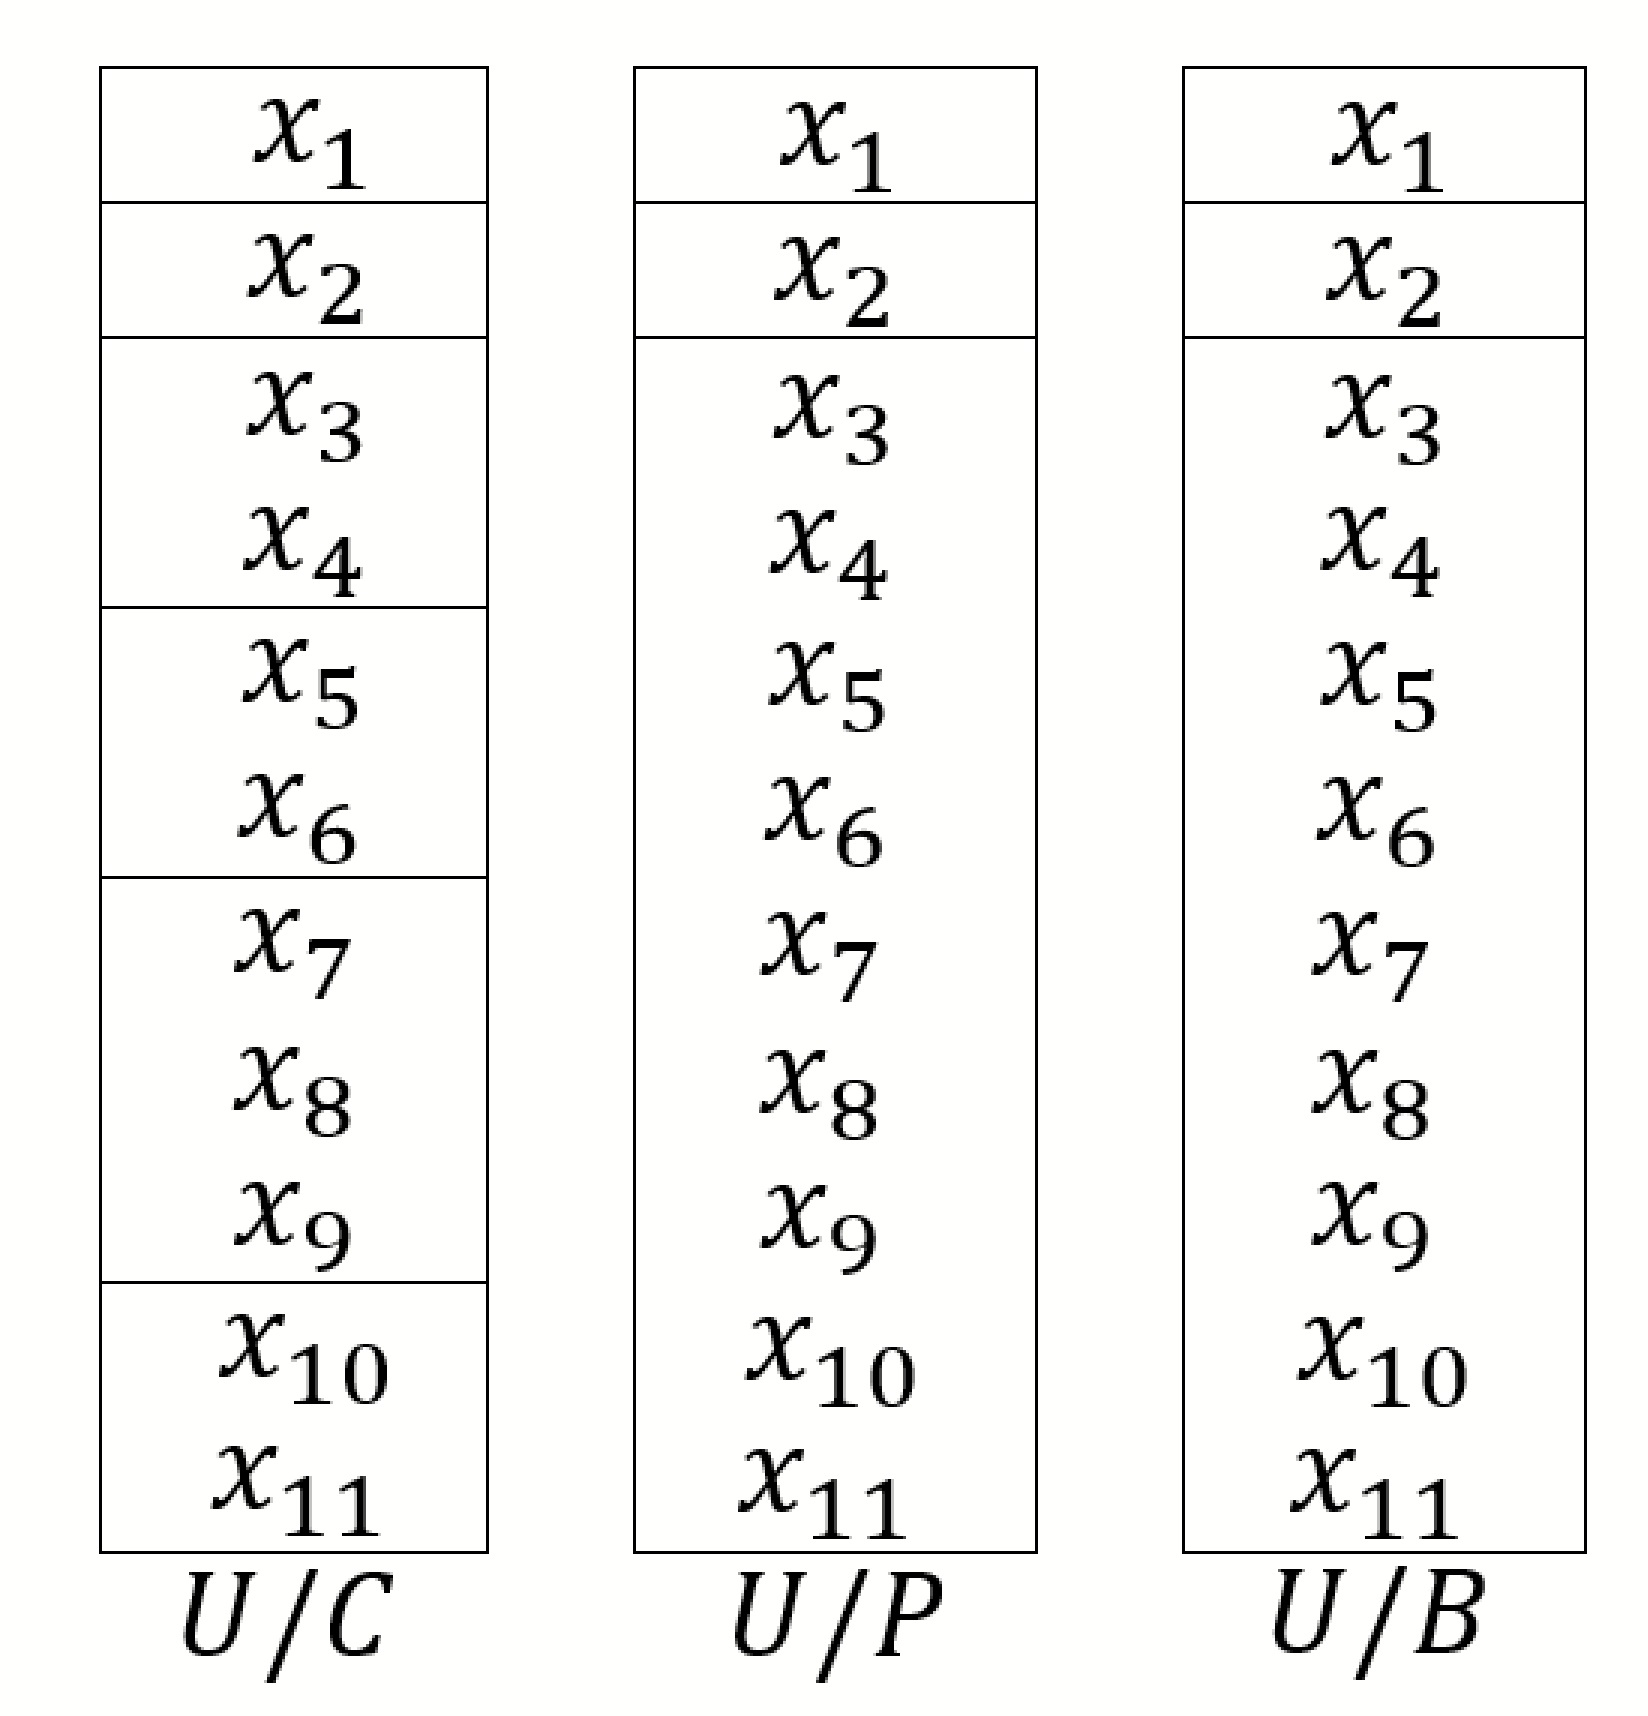
\includegraphics[width=5cm]{./12.jpg} 
			\caption{Granularity comparison}
			\label{GSComparison}
		\end{figure}
		\par To help the understanding of the proposed algorithms, here we show the process of algorithm \ref{GS} for obtaining a positive region preservation reduct.
		\\\textbf{An example of algorithm \ref{CTGKC} for computing the target granularity.}\\
		Considering $X_1 \subset {\rm POS}_C(D)$, we have $\forall x \in X_1, {\rm Key}(x,PRPR)=f(x_1,d)=1, {\rm Key}_a(1).add(x_1)=\{x_1\}$.\\
		Considering $X_2 \subset {\rm POS}_C(D)$, we have $\forall x \in X_2, {\rm Key}(x,PRPR)=f(x_2,d)=2, {\rm Key}_a(2).add(x_2)=\{x_2\}$.\\
		Considering $X_3 \subset {\rm BND}_C(D)$, we have $\forall x \in X_3, {\rm Key}(x,PRPR)=4, {\rm Key}_a(4).add(X_3)\\=\{x_3,x_4\}$.\\
		Considering $X_4 \subset {\rm BND}_C(D)$, we have $\forall x \in X_4, {\rm Key}(x,PRPR)=4, {\rm Key}_a(4).add(X_4)\\=\{x_3,x_4,x_5,x_6\}$.\\
		Considering $X_5 \subset {\rm BND}_C(D)$, we have $\forall x \in X_5, {\rm Key}(x,PRPR)=4, {\rm Key}_a(4).add(X_5)\\=\{x_3,x_4,x_5,x_6,x_7,x_8,x_9\}$.\\
		Considering $X_6 \subset {\rm BND}_C(D)$, we have $\forall x \in X_6, {\rm Key}(x,PRPR)=4, {\rm Key}_a(4).add(X_6)\\=\{x_3,x_4,x_5,x_6,x_7,x_8,x_9,x_{10},x_{11}\}$.\\
		Finally, we get ${\rm Key}_a(1)=\{x_1\},{\rm Key}_a(2)=\{x_2\},{\rm Key}_a(4)=\{x_3,x_4,x_5,x_6,x_7,x_8,x_9,x_{10},
		\\x_{11}\}$ and ${\rm TGran}(PRPR)=\{\{x_1\},\{x_2\},\{x_3,x_4,x_5,x_6,x_7,x_8,x_9,x_{10},x_{11}\}\}$.
		\\\textbf{An example for calculating core attributes.}\\% of algorithm \ref{CCARS}
		According to Algorithm \ref{CTGKC}, we get $G={\rm TGran}(PRPR)=\{\{x_1\},\{x_2\},\{x_3,x_4,
		\\\cdots,x_{11}\}\}$.
		Firstly, we compute the partition of $U$ determined by $C$, \emph{i.e.,} $U/C=\lbrace X_{1},X_{2},X_{3},X_{4},X_{5},X_{6} \rbrace=\lbrace \lbrace x_{1} \rbrace,\lbrace x_{2} \rbrace,\lbrace x_{3},x_{4} \rbrace,\lbrace x_{5},x_{6} \rbrace,
		\lbrace x_{7},x_{8},x_{9} \rbrace,\lbrace x_{10},x_{11} \rbrace \rbrace.$
		Secondly, we calculate the significance of every element of $C$ to determine whether the element is a core attribute or not. For attribute $a_1$, we have $U/C-\{a_1\}=\{\{x_1,x_2\},\{x_3,x_4\},\{x_5,x_6\},\{x_7,x_8,x_9\},\{x_{10},x_{11}\}\}$ and $ Sig^-(a_1,C,G)=|U-\{x_3,\cdots,x_{11}\}|=2$. According to $Sig^-(a_1,C,G)>0$, we know that $a_1$ is a core attribute.
		For attribute $a_2$, we have $U/C-\{a_2\}=\{\{x_1\},\{x_2,x_3,x_4\},\{x_5,x_6\},\\\{x_7,x_8,x_9\},\{x_{10},x_{11}\}\}$ and $ Sig^-(a_2,C,G)=|U-\{x_1,x_5,x_6,\cdots,x_{11}\}|=3$. According to $Sig^-(a_2,C,G)>0$, we know that $a_2$ is a core attribute.
		For attribute $a_3$, we have $U/C-\{a_3\}=\{\{x_1\},\{x_2,x_3,x_4\},\{x_5,x_6\},\{x_7,x_8,x_9,x_{10},x_{11}\}\}$ and 
		$Sig^-(a_3,C,G)=0$. As a result, we know $a_3$ is not a core attribute.
		For attribute $a_4$, we have $U/C-\{a_4\}=\{\{x_1\},\{x_2,x_3,x_4\},\{x_5,x_6,x_7,x_8,x_9\},\{x_{10},x_{11}\}\}$ and
		$Sig^-(a_4,C,G)=0$. So we know $a_4$ is not a core attribute.
		For attributes $a_5$ and $a_6$, we have $U/C-\{a_5\}=U/C-\{a_6\}=\{\{x_1\},\{x_2\},\{x_3,x_4\},\{x_5,x_6\},\{x_7,x_8,\\x_9\},\{x_{10},x_{11}\}\}$ and	$Sig^-(a_5,C,G)=Sig^-(a_6,C,G)=0$. Thus, neither $a_5$ nor $a_6$ is not a core attribute. 
		Finally we get $core=\{a_1,a_2\}$
		\\\textbf{Example of algorithm\ref{GS} for obtaining a positive region preservation reduct.}\\
		Now we get $G={\rm TGran}(PRPR)=\{\{x_1\},\{x_2\},\{x_3,x_4,\cdots,x_6\}\}$ and $reduct=core=\{a_1,a_2\}$. As a result, we can get $U=U-{\rm GA}(reduct)=\emptyset$. Because $U$ is $\emptyset$,  Algorithm\ref{GS} outputs $reduct=\{a_1,a_2\}$.
		 
\section{Experiments and analyses}\label{exps}
	\par The objective of following experiments in this section is to show the effectiveness and the efficiency of the attribute reduction algorithms, \emph{i.e.}, GS and GSV. Experiments are divided into three aspects. First, we employed 12 data sets in Table \ref{uci} to verify the performance of time consumption of GS, GSV, QGARA-FS, and QGARA-BS. Then, the computational time of algorithms GS, GSV, QGARA-FS and QGARA-BS with the increase of the size of objects and attributes was compared. Finally, we evaluated the classification accuracy of reducts generated by general attribute reduction algorithms using the naive bayes classifier and the decision tree classifier.
	\par We carried out all the attribute reduction algorithms in experiments on a personal computer with Windows 10, Intel(R) Core(TM) CPU i5-8265U 1.60GHZ and 8GB RAM memory. The software used was Visual Studio Code 1.3.8, and the programming language was Python 3.7.
	\begin{table}[htbp]
		\caption{UCI Data Sets}
		\label{uci}
		\begin{center}
			\begin{tabular}{cccccc}
				\hline
				ID & Data sets                  & cases& attributes & classes & $\gamma_C(D)$ \\ \hline
				1  & Shuttle           		    & 58000 & 10         & 7       & 0.230        \\
				2  & Mushroom                   & 5644  & 23         & 6       & 0.536        \\
				3  & Tic	                    & 9822  & 86         & 2       & 0.968        \\
				4  & Segmentation	     	    & 2310  & 20         & 7       & 0.989        \\
				5  & Pima-indians-diabetes		& 768   & 9          & 2       & 0.995        \\
				6  & Splice                     & 3190  & 61         & 3       & 0.999        \\
				7  & Dermatology                & 358   & 34         & 6       & 1             \\
				8  & Wdbc                  		& 569   & 31         & 2       & 1             \\
				9  & CNAE9                      & 1080  & 856        & 9       & 1             \\
				10 & Semeion                    & 1593  & 267        & 10      & 1             \\
				11 & DNA                        & 2000  & 181        & 3       & 1             \\
				12 & Connect4                   & 67557 & 43         & 3       & 1             \\
				\hline
			\end{tabular}
		\end{center}
	\end{table}
	\par The data sets used in experiments are all downloaded from UCI repository of machine learning data sets \cite{Dua:2019} whose basic information is outlined in Table \ref{uci}. For the sake that reduction algorithms can address only symbolic data, data sets containing continuous attributes ,\emph{i.e.}, Segmentation, Pima-indians-diabetes, and Wdbc, were preprocessed by equal-width discretization algorithms. For data sets with missing values,\emph{i.e.}, Mushroom,  we removed the objects with missing values to achieve uniform treatment of all data sets. The last column of Table \ref{uci}, \emph{i.e.}, $\gamma_C(D)$, stands for the positive region dependency degree $|{\rm POS}_C(D)|/|U|$. The data set is consistent when $\gamma_C(D)=1$; otherwise, the data set is inconsistent. As shown in Table \ref{uci}, Shuttle, Mushroom, Tic, Segmentation, Pima-indians-diabetes, and Splice are inconsistent and the other 6 data sets are consistent. Taking into consideration the similar results of five types of reducts under the general reduction algorithms, we mainly took positive region preservation reduction and relative discernibility relation preservation reduction results to verify the difference of four reduction algorithms.
	\subsection{Efficiency comparison of four general attribute reduction algorithms}
		\par In this subsection, to show the time efficiency of proposed algorithms, we presented the time consumption of four attribute reduction algorithms in obtaining reducts, and experiments results were shown in Tables \ref{prprTime} and \ref{drprTime}.
		\par Table \ref{prprTime} indicated the computational time of QGARA-FS, QGARA-BS, GS, and GSV for obtaining a positive region preservation reduct on 12 data sets. We can see that GSV was the fastest in four attribute reduction algorithms, and GS was faster than QGARA-FS. From results of experiments on both consistent and inconsistent decision tables, the computational time of four algorithms in obtaining positive region preservation reduct followed this order: QGARA-FS $\geq$ GS, QGARA-FS $> $ GSV. GS performed better than QGARA-BS on small-scale data sets. However, in processing the large-scale data, it consumed more time than QGARA-BS for that the computation of the attribute with maximal significance was time-consuming. For most of the cases in experiments, the computational time of GS can reduce over half the computation time of QGARA-FS, such as data sets 2(Mushroom), 3(Tic), 4(Segmentation), etc. In the same condition, GSV can reduce over half of the computation time of QGARA-BS, such as data sets 5(Pima-indians-diabetes), 7(Dermatology), 9(CNAE9), etc.
		\begin{table}[htb]
			\centering
			\caption{Time consumption for obtaining PRPR.}
			\label{prprTime}
			\begin{tabular}{ccccc}
				\hline
				\multirow{2}{*}{ID} & Time of     & Time of & Time of     & Time of \\
				& QGARA-FS(s) & QGARA-BS(s)   & GS(s) & GSV(s)  \\ \hline
	      		1   &  9.326     & 7.967  & 6.562   & \textbf{1.676} \\
				2   &  11.788    & 1.990   & 1.816   & \textbf{0.213} \\
				3   &  192.414   & 18.784 & 17.890   & \textbf{1.581} \\
				4   &  1.215     & 0.772  & 0.521   & \textbf{0.117} \\
				5   &  0.123     & 0.109  & 0.067   & \textbf{0.018} \\
				6   &  27.328    & 3.790   & 5.638   & \textbf{0.406} \\
				7   &  1.139     & 0.216  & 0.233   & \textbf{0.024} \\
				8   &  1.533     & 0.272  & 0.259   & \textbf{0.040 } \\
				9   &  1095.294  & 67.414 & 129.634 & \textbf{2.199} \\
				10  &  162.241   & 13.839 & 35.478  & \textbf{2.247} \\
				11  &  94.026    & 9.592  & 21.678  & \textbf{3.702} \\
				12  &  889.698   & 61.010  & 137.170  & \textbf{17.500 } \\ \hline
			\end{tabular}
		\end{table}
		In summary, for calculating positive region preservation reducts on the consistent and inconsistent decision tables, the general attribute reduction algorithms proposed in this paper, \emph{i.e.} GS and GSV, were more efficient than the existing general attribute reduction algorithms, \emph{i.e.}, QGARA-FS and QGARA-BS.
		\begin{table}[htb]
			\centering
			\caption{Time consumption for obtaining DRPR.}
			\label{drprTime}
			\begin{tabular}{ccccc}
				\hline
				\multirow{2}{*}{ID} & Time of     & Time of & Time of     & Time of \\
				& QGARA-FS(s) & QGARA-BS(s)   & GS(s) & GSV(s)  \\ \hline
				1   & 10.885  & 9.831  & 7.489    & \textbf{4.103} \\
				2   & 3.640    & 2.419  & 2.064    & \textbf{1.864} \\
				3   & 200.923 & 19.734 & 19.231   & \textbf{3.168} \\
				4   & 1.423   & 0.925  & 0.648    & \textbf{0.244} \\
				5   & 0.157   & 0.140   & 0.099    & \textbf{0.044} \\
				6   & 29.326  & 4.279  & 6.016    & \textbf{0.794} \\
				7   & 1.145   & 0.263  & 0.258    & \textbf{0.051} \\
				8   & 1.570    & 0.357  & 0.312    & \textbf{0.065} \\
				9   & 1152.034& 70.652 & 129.052  & \textbf{2.061} \\
				10  & 175.911 & 14.870 & 36.988   & \textbf{2.057} \\
				11  & 95.743  & 10.190 & 20.596   & \textbf{3.522} \\
				12  & 894.983 & 60.119 & 132.542  & \textbf{16.472} \\ \hline
			\end{tabular}
		\end{table}
		\par Table \ref{drprTime} shows the time consumption of four general reduction algorithms for obtaining a relative discernibility relation preservation reduct. For the consistent decision table, a positive region preservation reduct is also a relative discernibility relation preservation reduct. Thus, the results of the time consumption of four general reduction algorithms on six consistent data sets were similar to the statistics of Table \ref{prprTime}. For the time consumption of general reduction algorithms on six inconsistent data sets, we can know that the computational time of GS was less than that of QGARA-FS, and the same condition to GSV and QGARA-BS. In brief, the results of Table \ref{drprTime} were consistent with the observations of Table \ref{prprTime}. In summary, for calculating relative discernibility relation preservation reduct on the consistent and inconsistent decision tables, the general reduction algorithms proposed in this paper were more efficient than the existing general reduction algorithms. 
	\subsection{Comparison of reduction algorithms for different proportion data sets}
		\par In this subsection, to further compare the efficiency of general reduction algorithms, we compared the computational time of QGARA-FS, QGARA-BS, GS, and GSV for obtaining a positive region preservation reduct with the increase of the size of objects and the size of attributes. 
		\par Figure \ref{TimeIncreaseObjects} shows detailed change trends of the time consumption of each algorithm for obtaining a positive region preservation reduct with the number of objects increasing. In Figure \ref{TimeIncreaseObjects}, the x-coordinate denotes the percentages of objects to the universe, while the y-coordinate concerns the time consumption of algorithms. We employed 8 data sets with different scale (Mushroom, Tic, Splice, Dermatology, Wdbc, CNAE9, DNA, and Connect4) to verify the performance of time consumption of QGARA-FS, QGARA-BS, GS, and GSV. Generally speaking, the computational time of four algorithms increased with the increase of the percentages of objects to the universe. The same as \cref{prprTime,drprTime}, GS was more efficient than QGARA-FS and GSV was faster than QGARA-BS.
		When dealing with the same UCI data sets, it is often the case that the computational time of GS was less than that of QGARA-FS, and equal to that of QGARA-BS for small-scale data. But in presence of large-scale data sets, QGARA-BS performed better than GS. It can be observed in many data sets, such as Figure \ref{TimeIncreaseObjects} (c), (e), (g).  The computational time of GSV was less than that of the other three general reduction algorithms. The computational time of QGARA-FS increased distinctly in comparison to GS when the number of objects was increasing; the computational time of QGARA-BS increased distinctly in comparison to GSV when the number of objects was increasing. 
		\begin{figure}[htbp] 
			\centering 
%			\subfigure[Shuttle]{
%				\label{Fig.sub1.1}
%				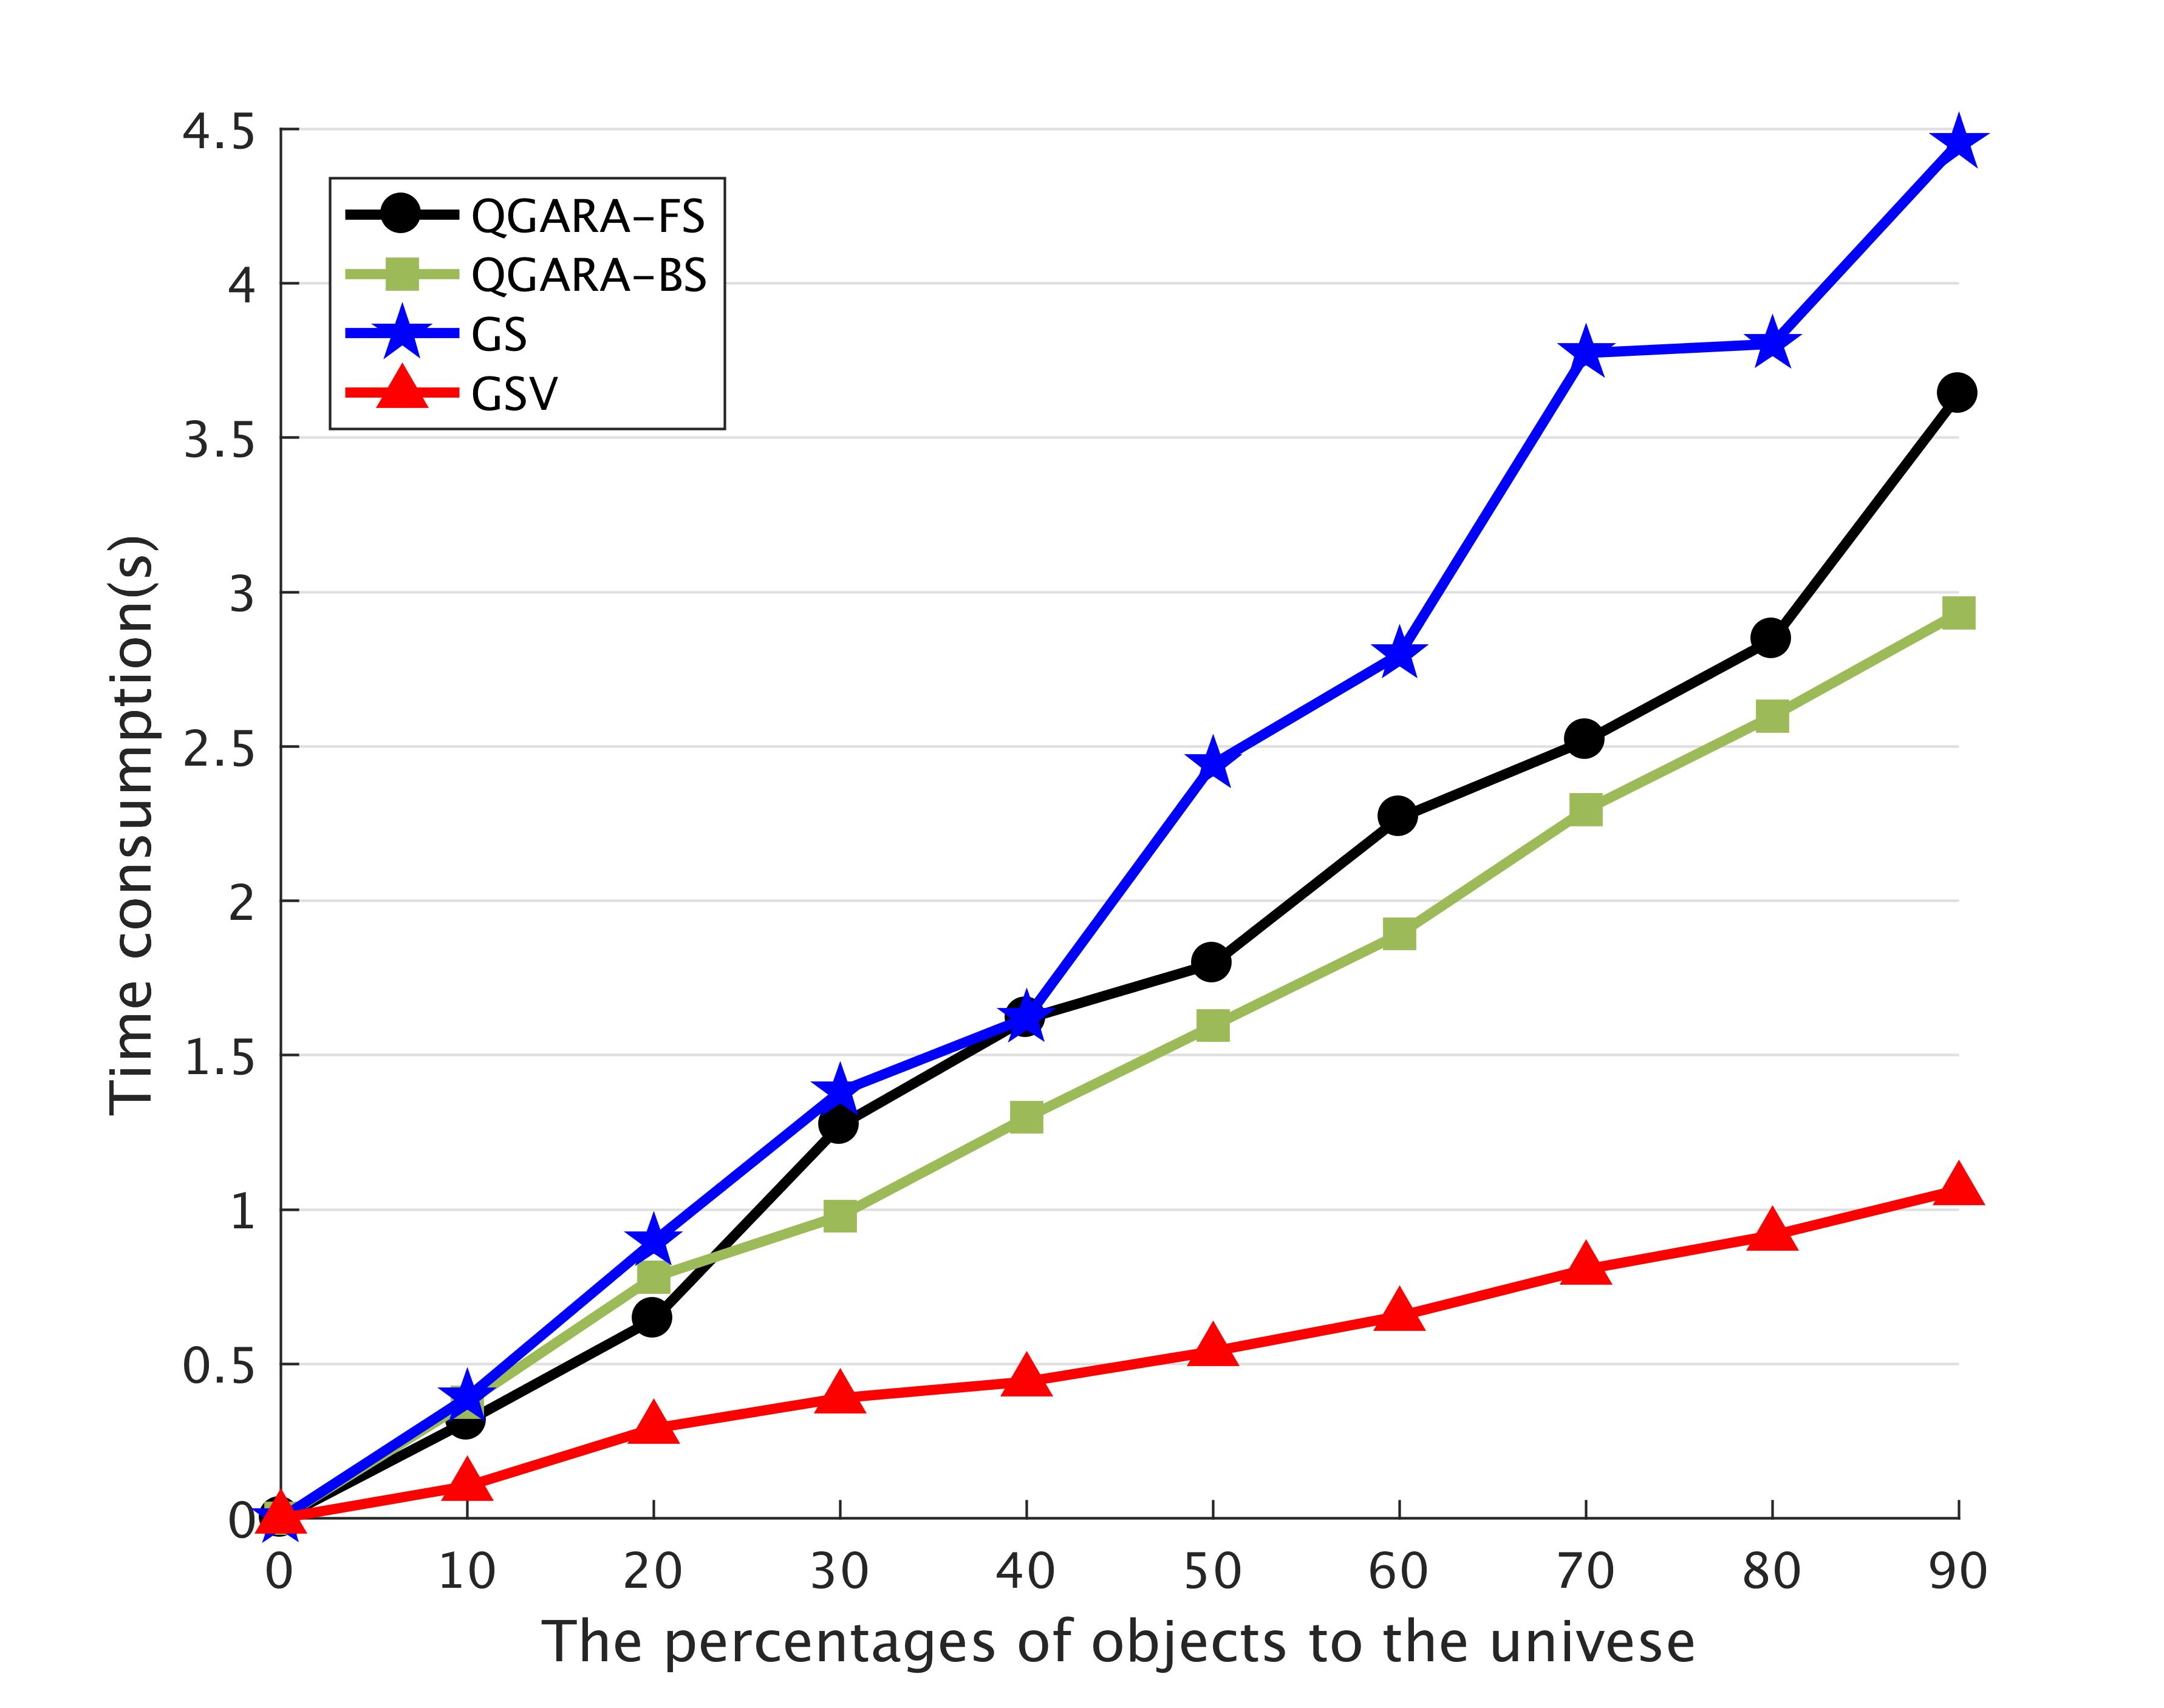
\includegraphics[width=5cm]{./Curve_universe/1.jpg} 
%			}
			\subfigure[Mushroom]{
				\label{Fig.sub1.2}
				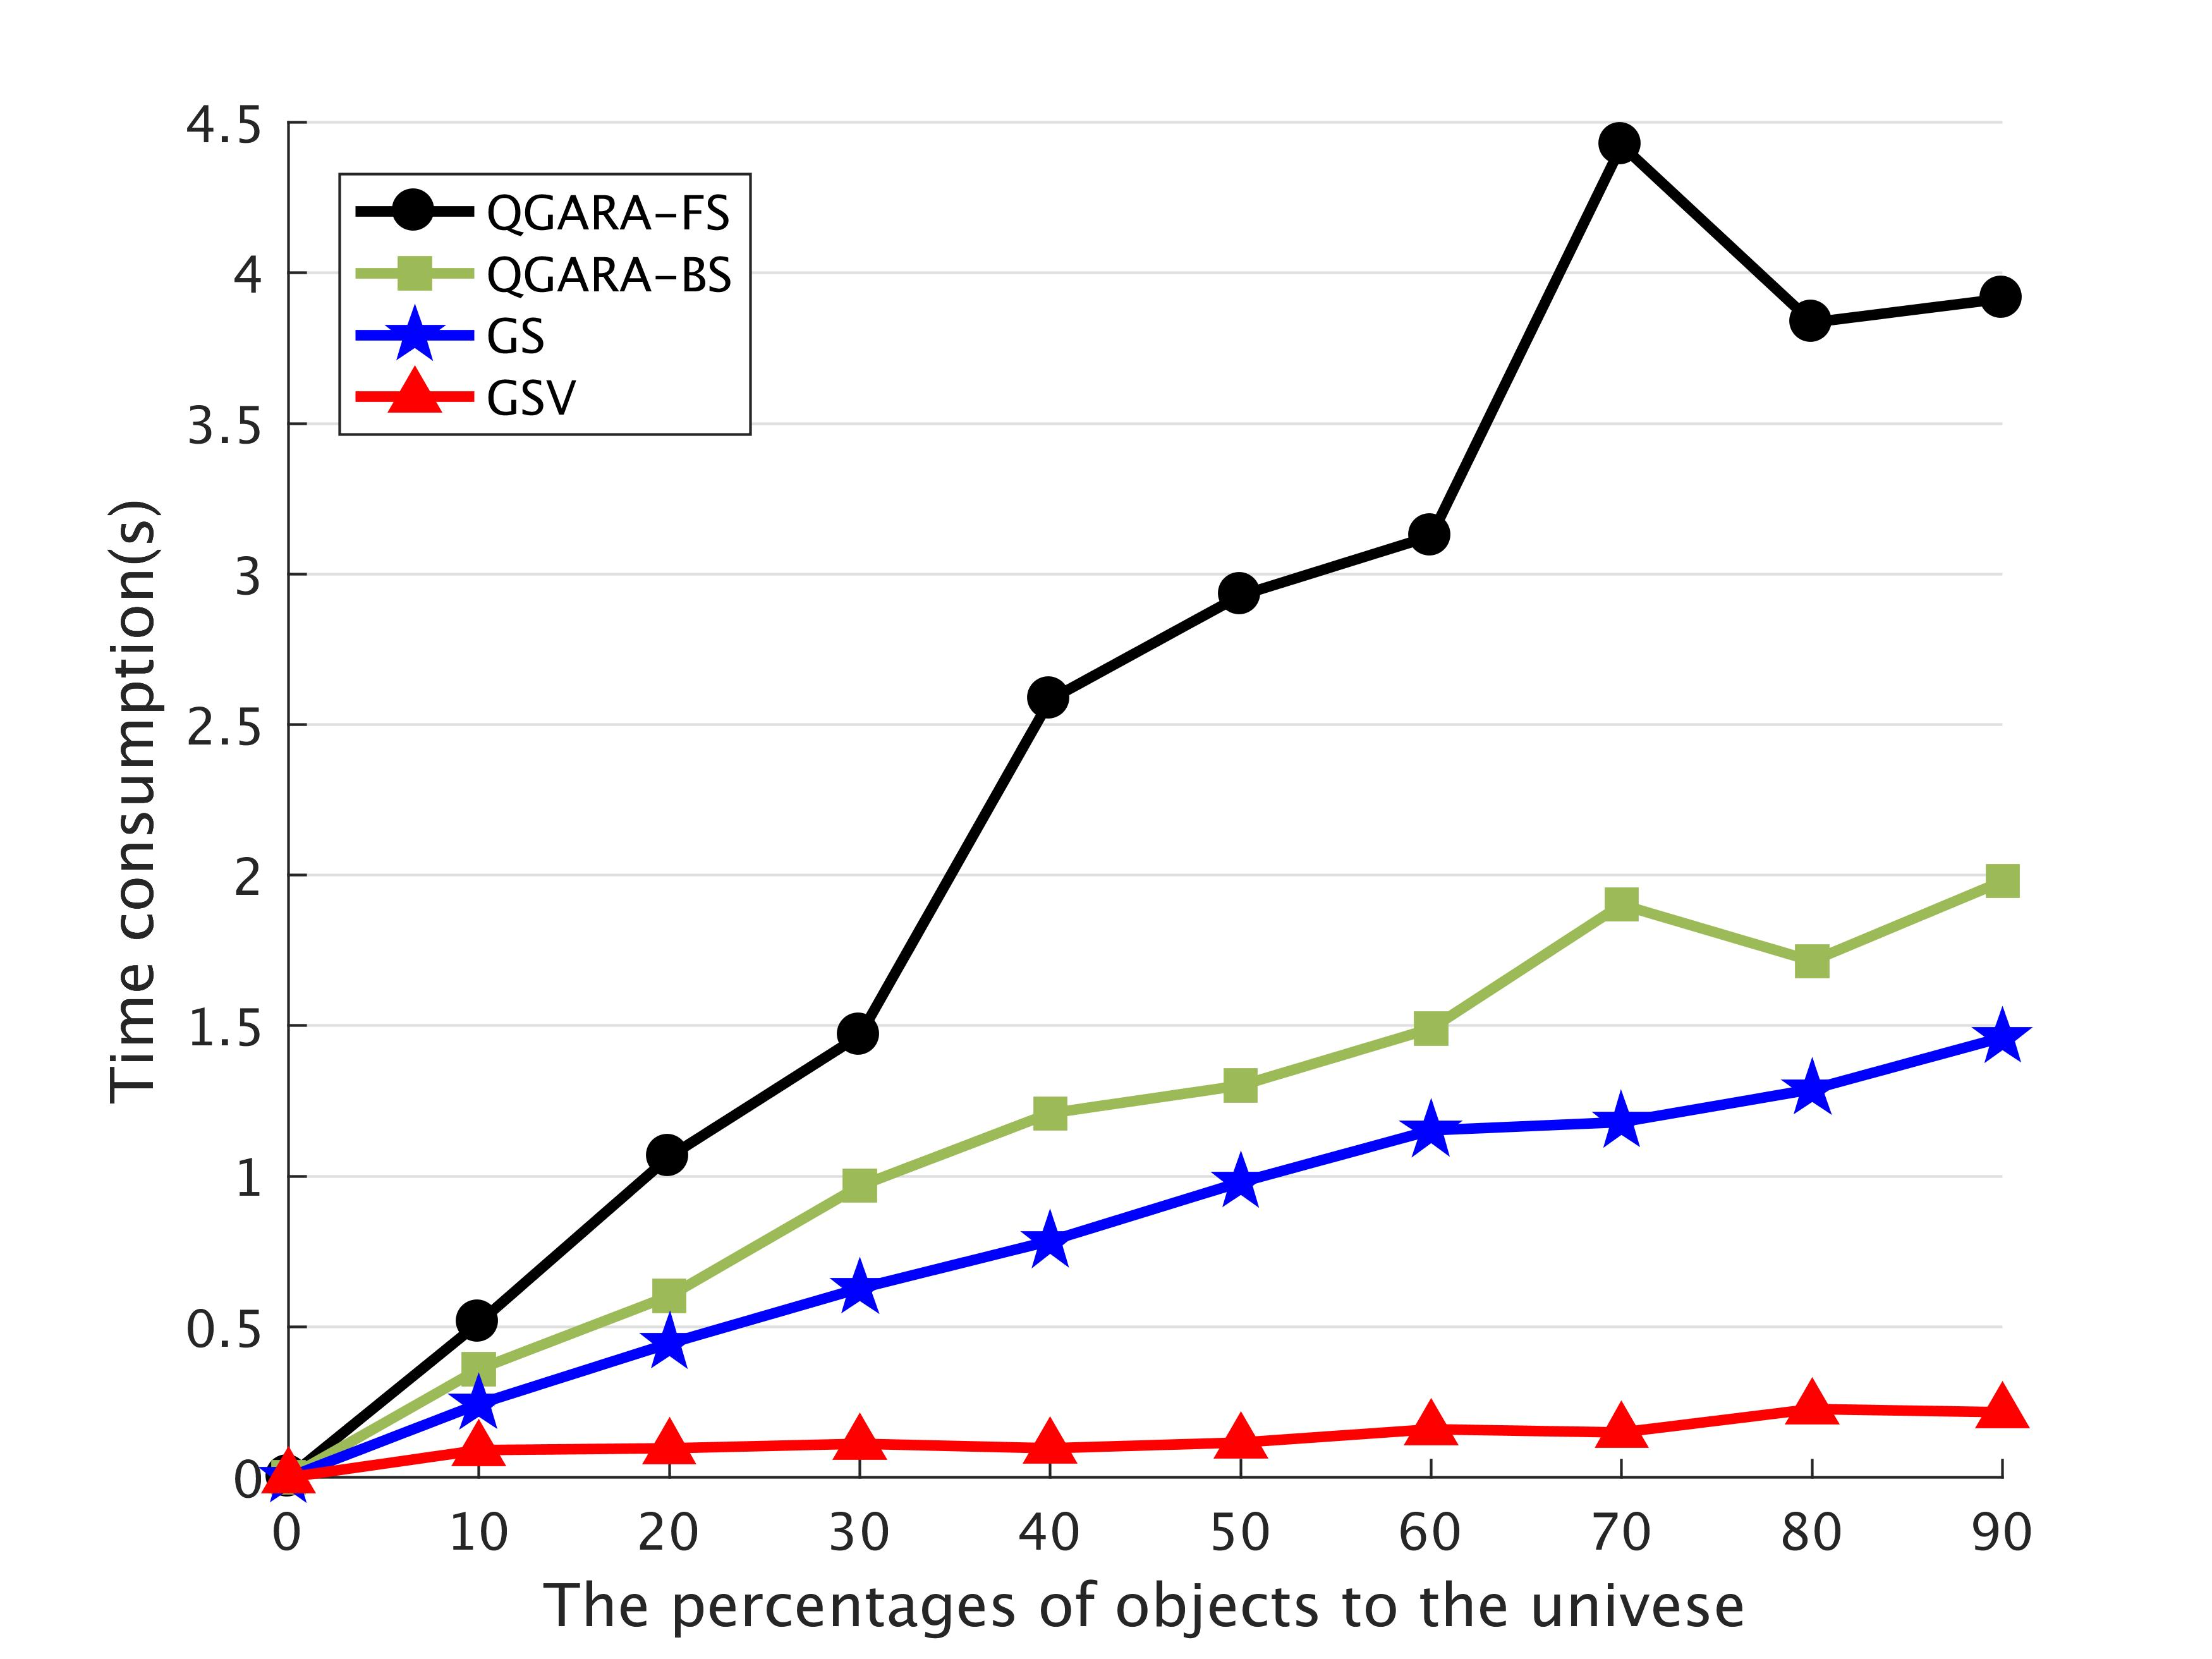
\includegraphics[width=5cm]{./Curve_universe/1_mushroom_pos.jpg} 
			}
			\subfigure[Tic]{
				\label{Fig.sub1.3}
				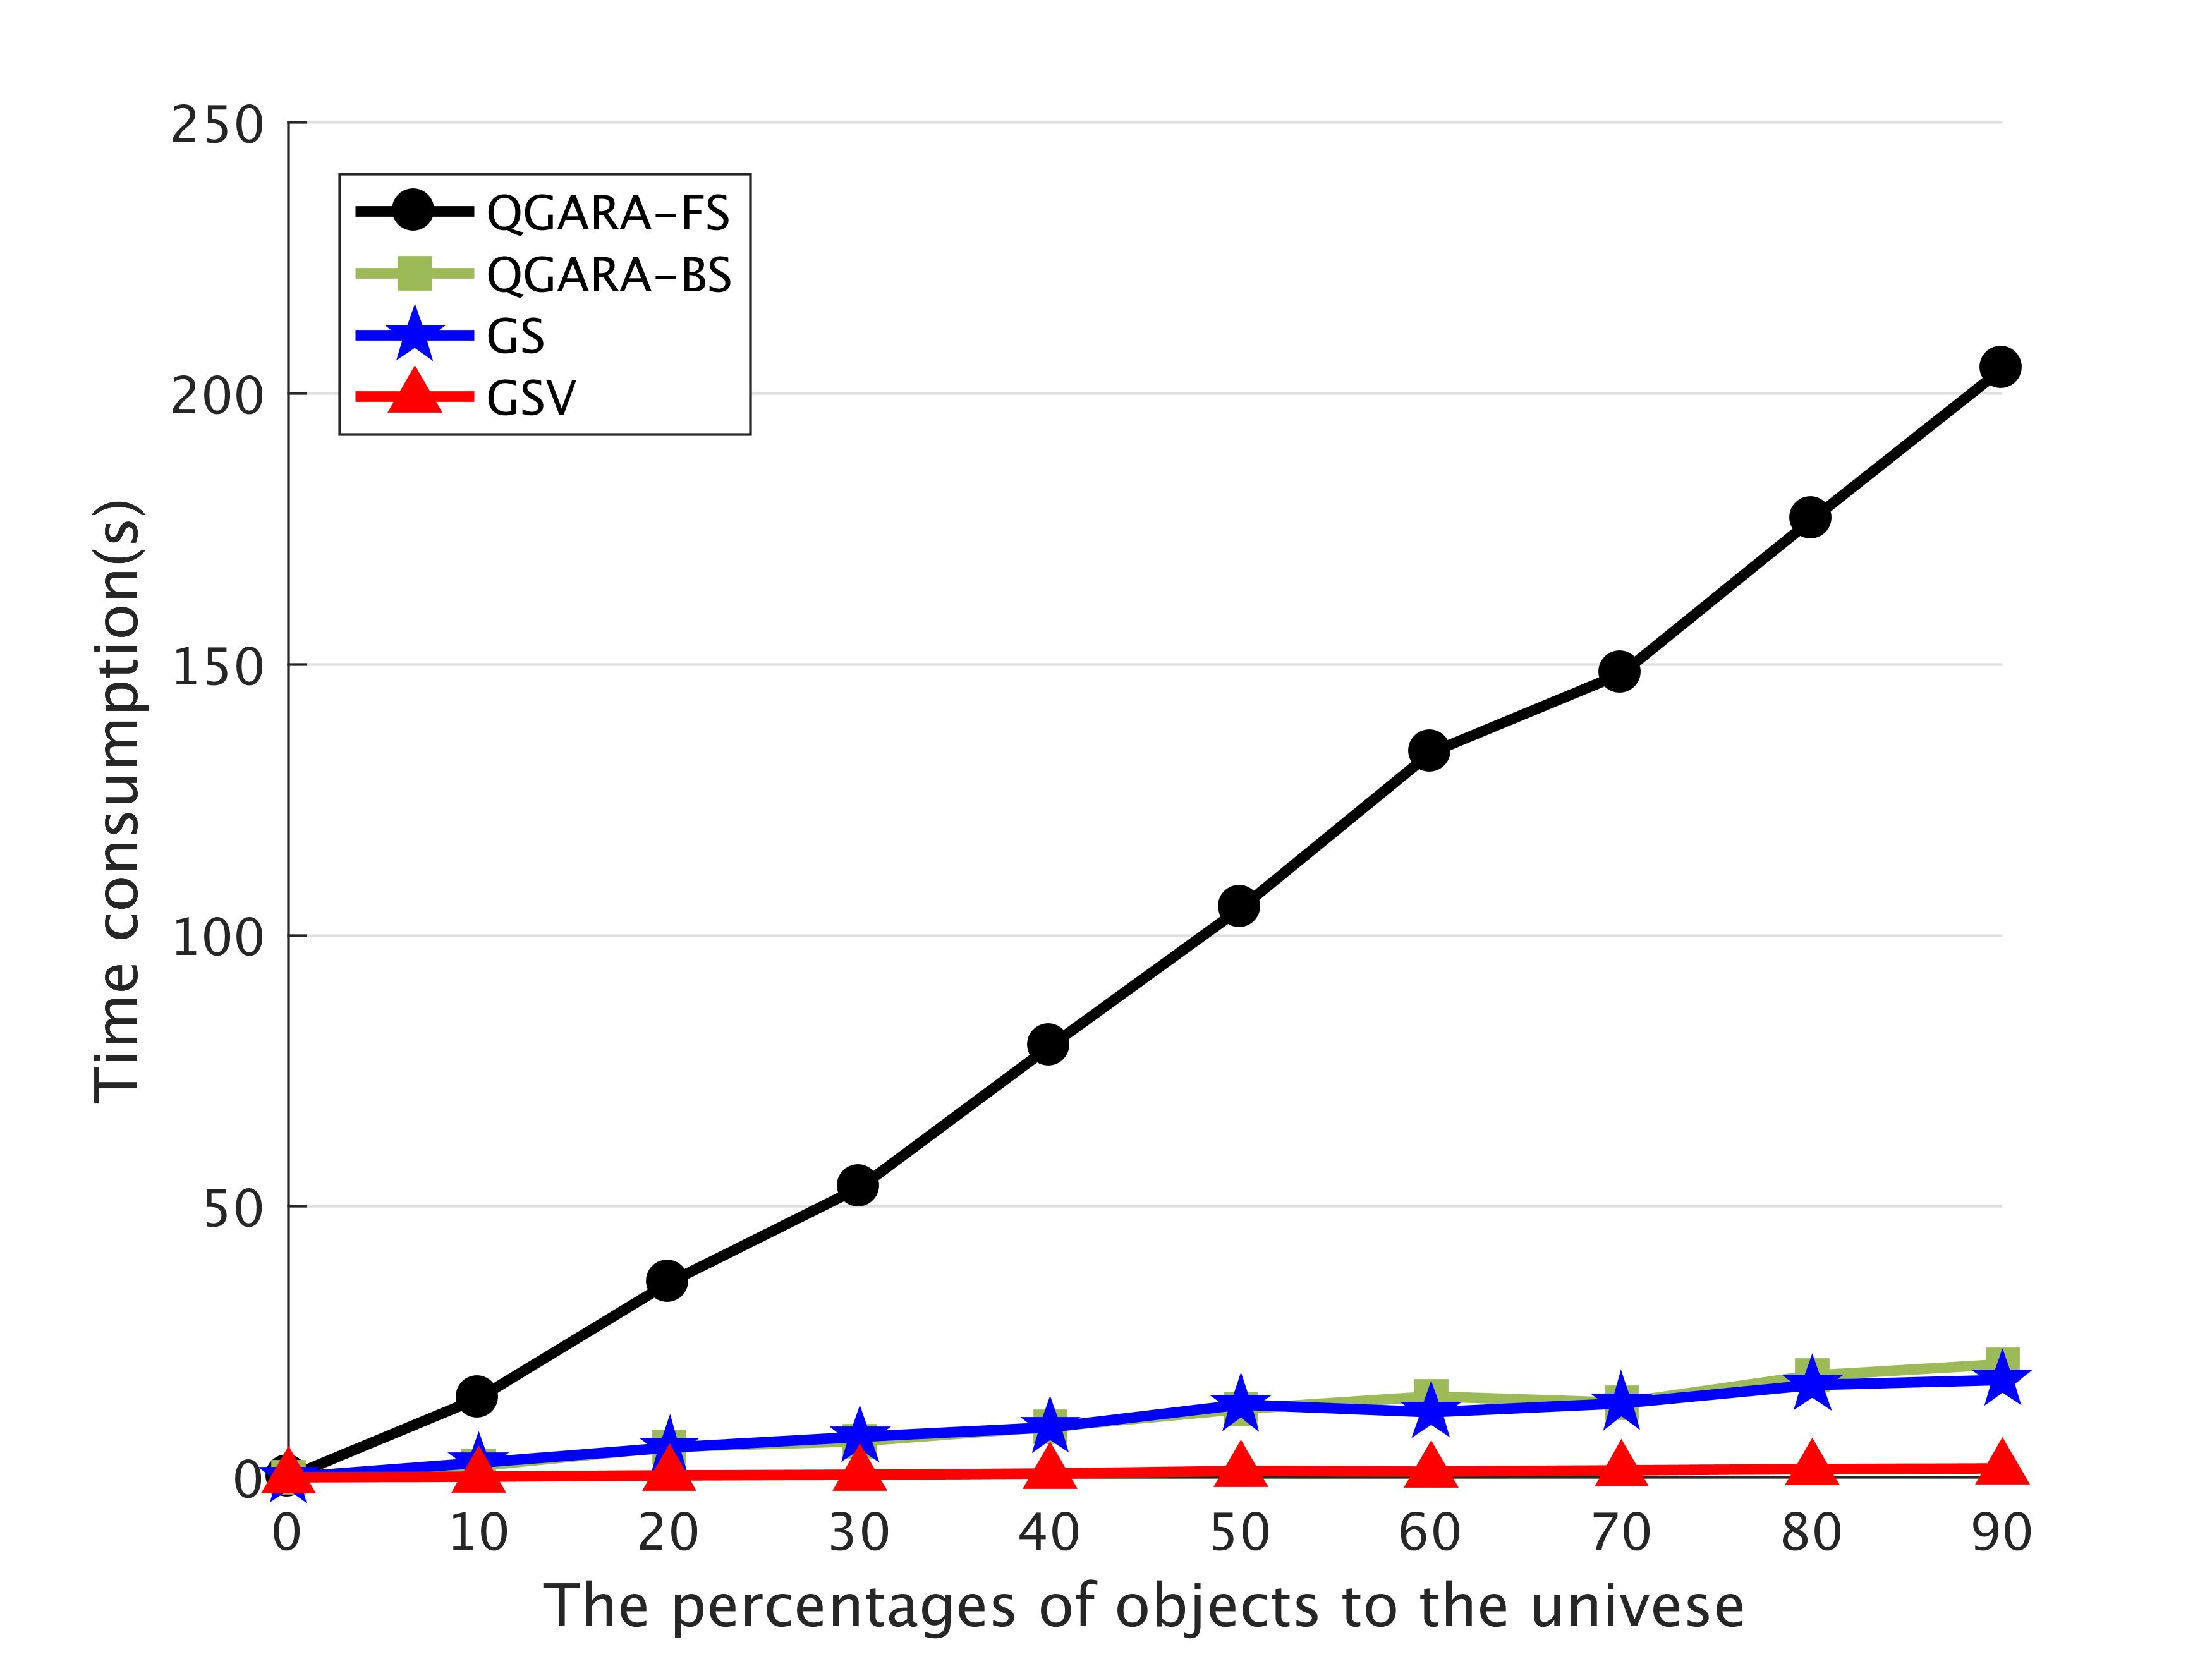
\includegraphics[width=5cm]{./Curve_universe/2_tic_pos.jpg} 
			}
%			\subfigure[Segmentation]{
%				\label{Fig.sub1.4}
%				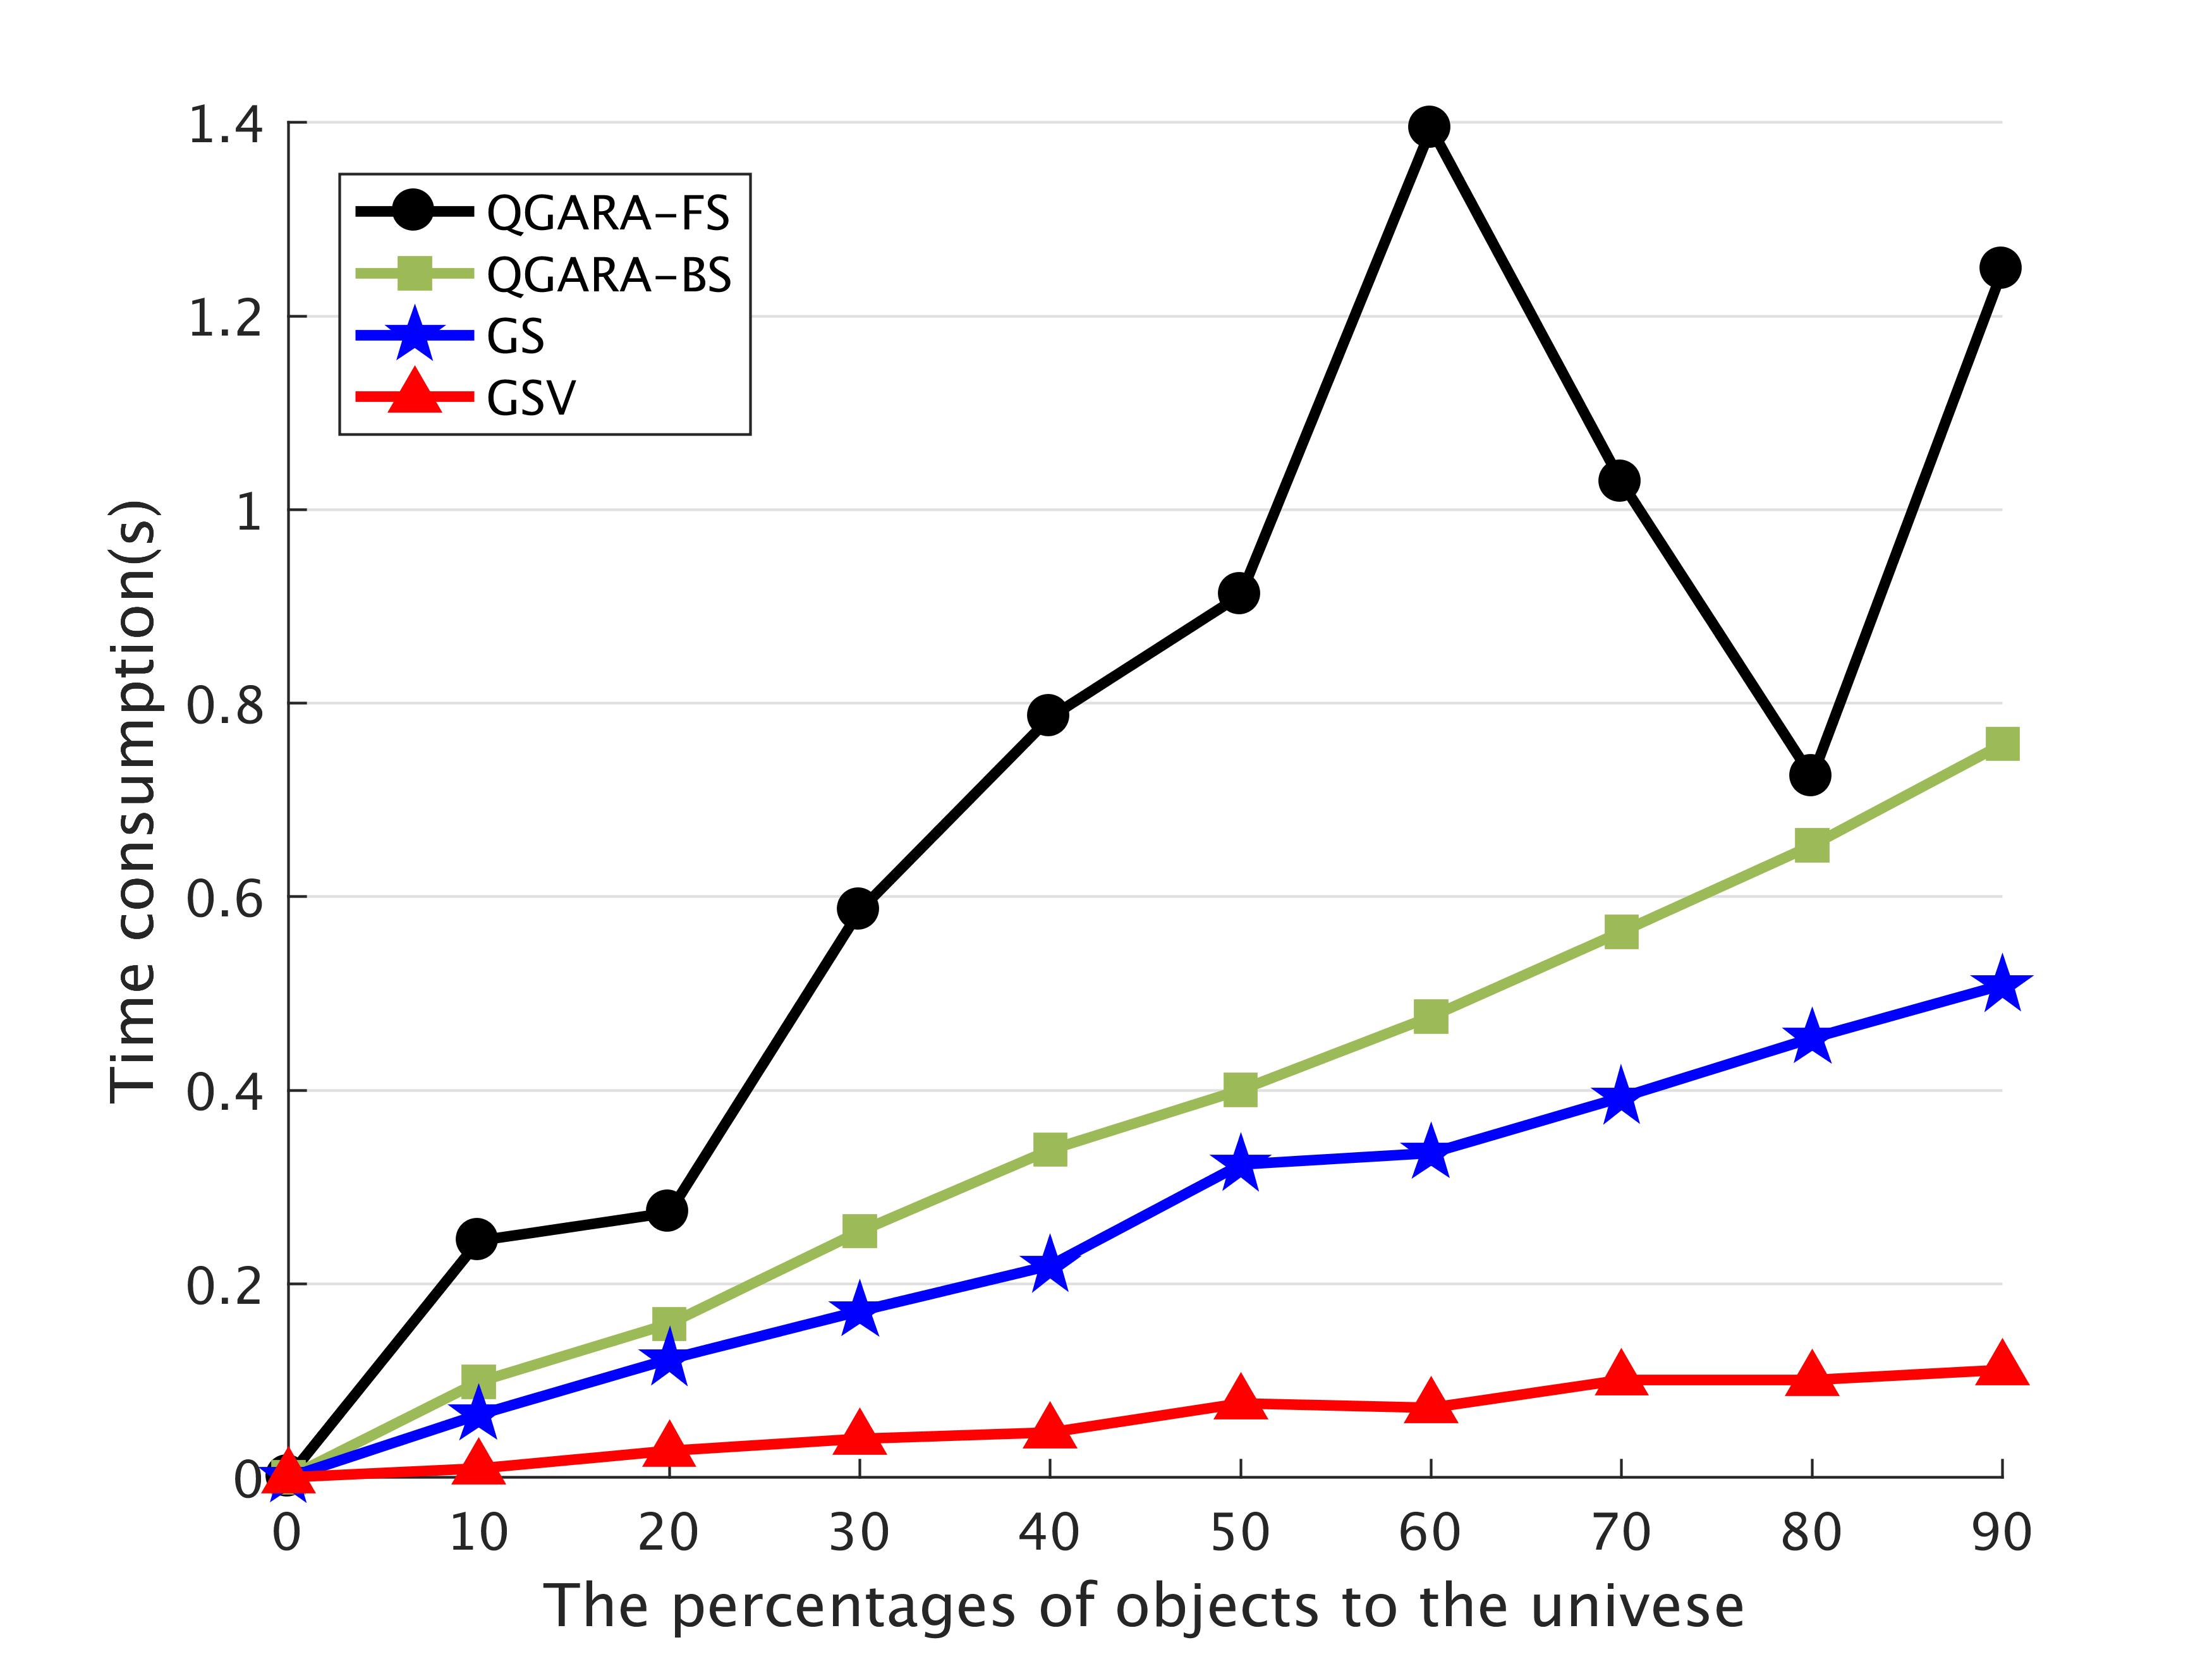
\includegraphics[width=5cm]{./Curve_universe/3_seg_pos.jpg} 
%			}
	%		\subfigure[pid(int)]{
	%			\label{Fig.sub1.5}
	%			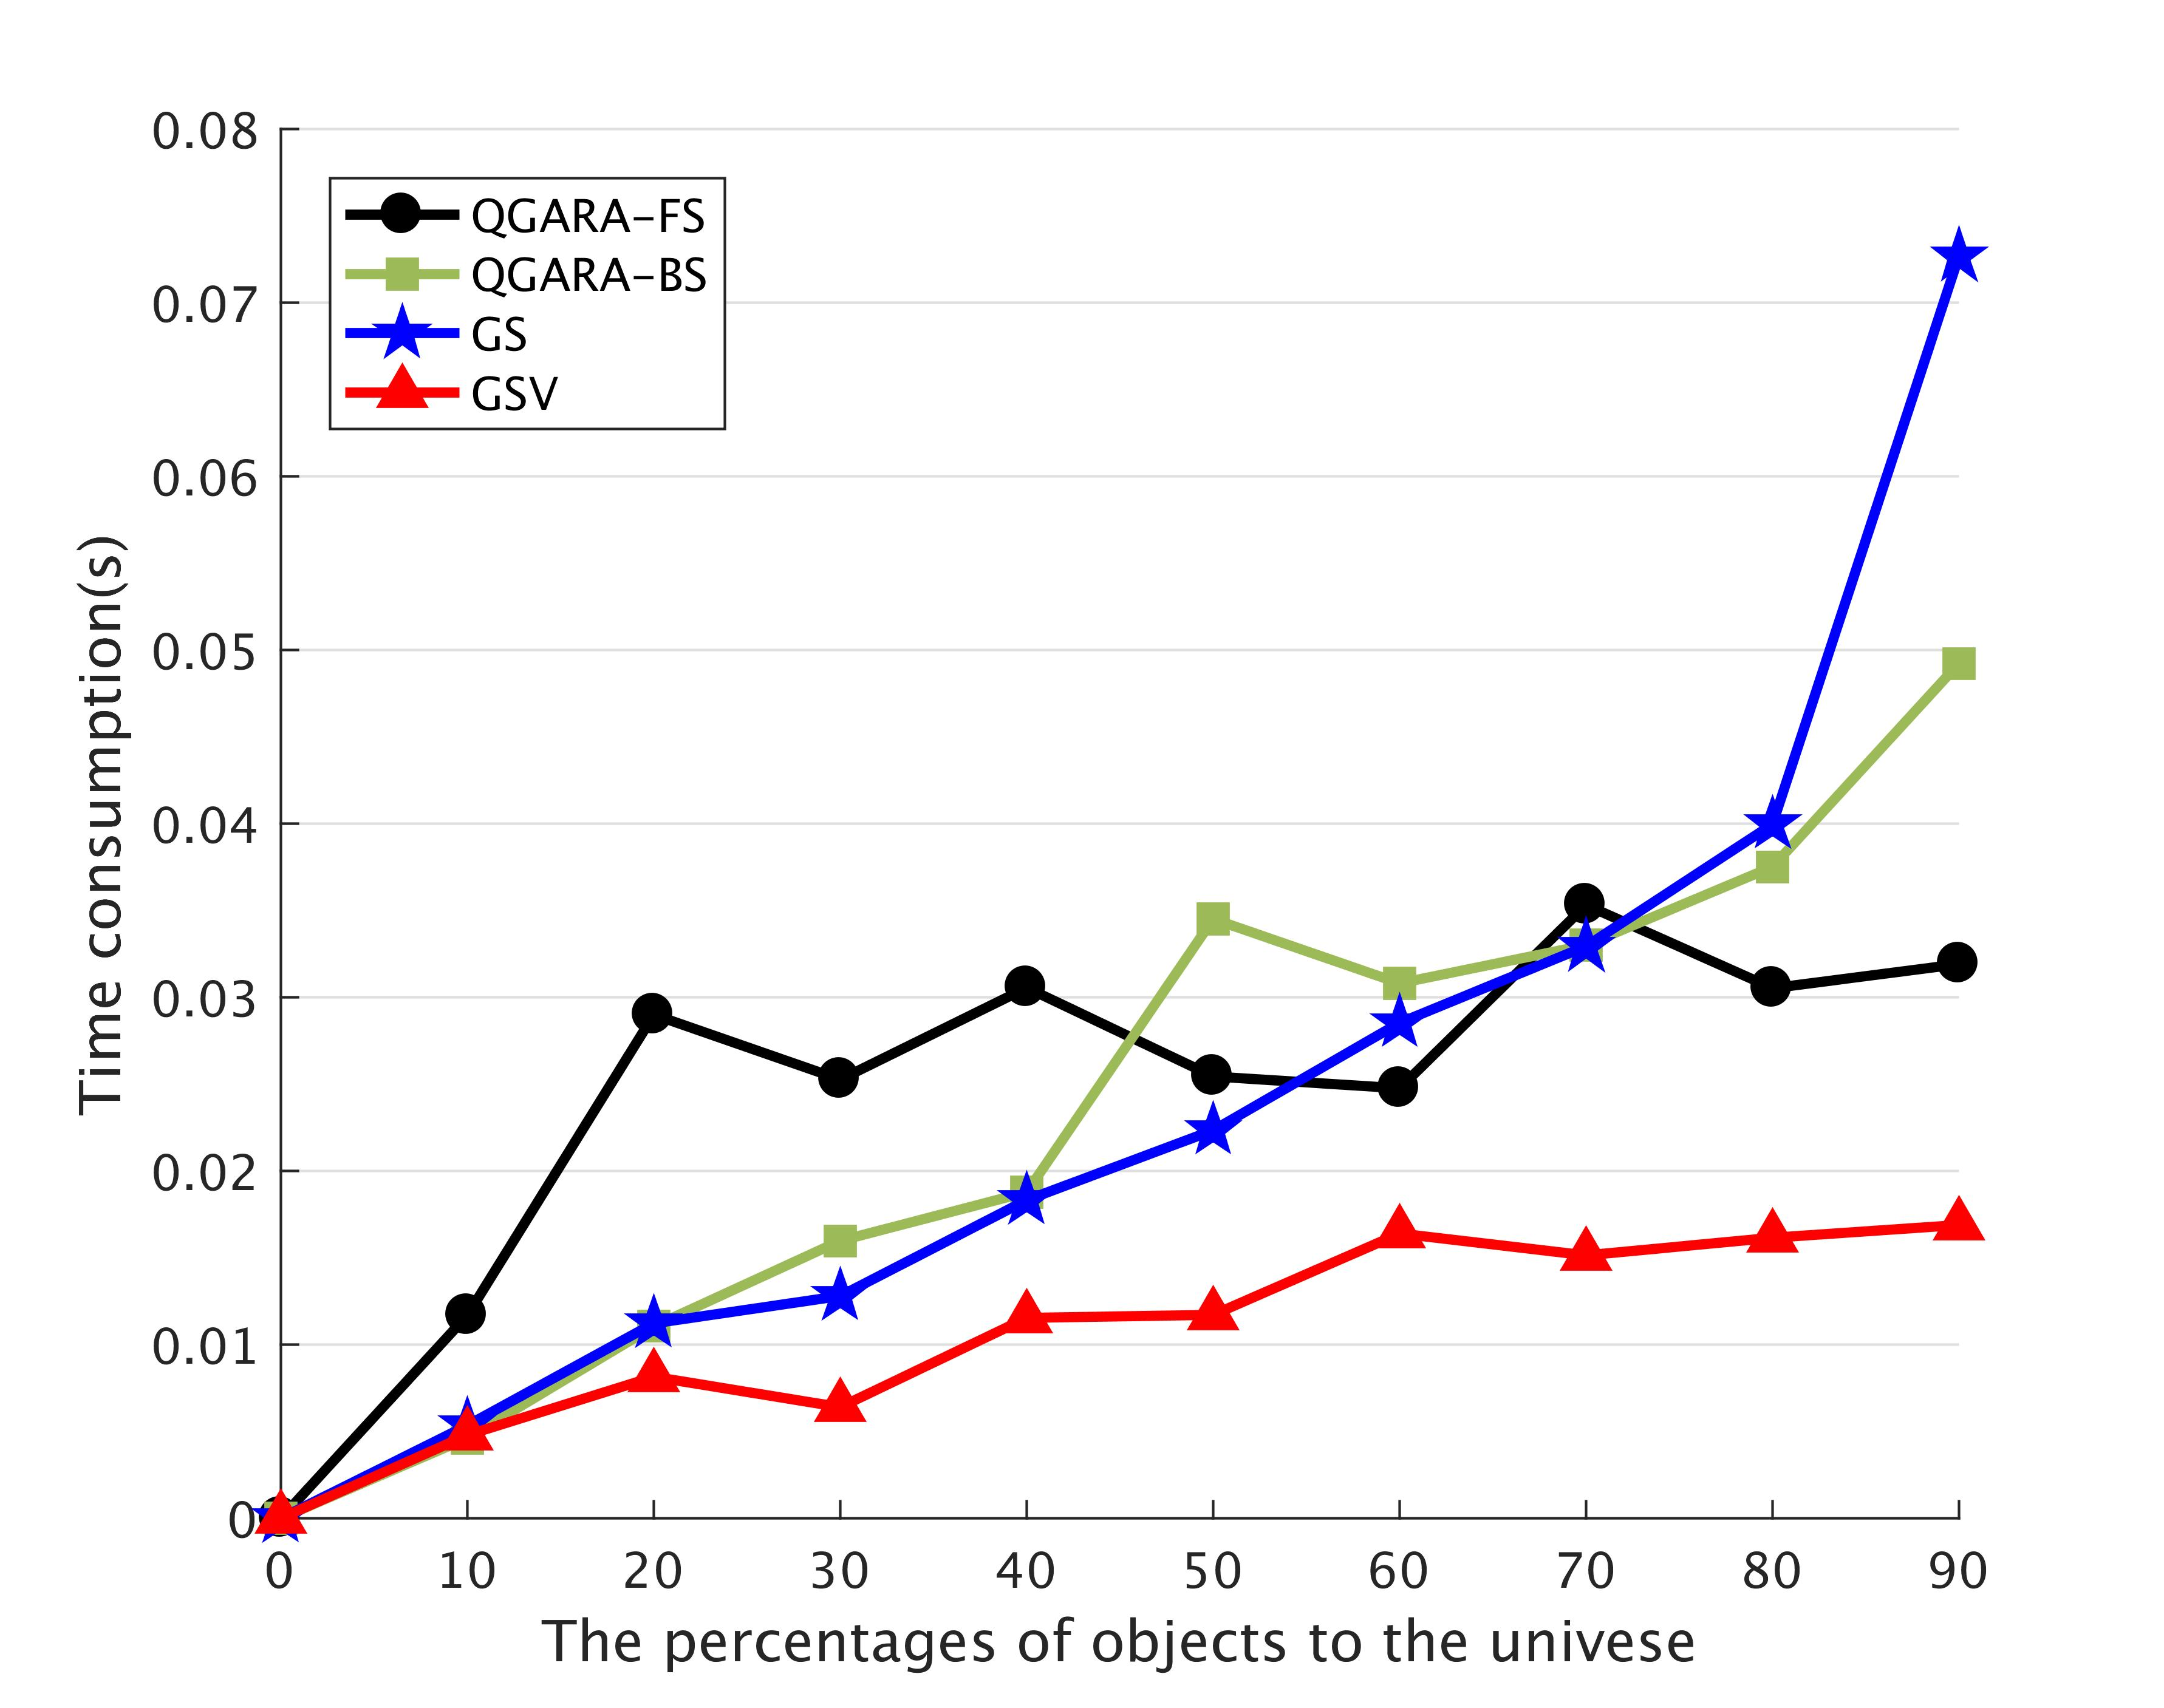
\includegraphics[width=5cm]{./Curve_universe/5.jpg} 
	%		}
			\subfigure[Splice]{
				\label{Fig.sub1.6}
				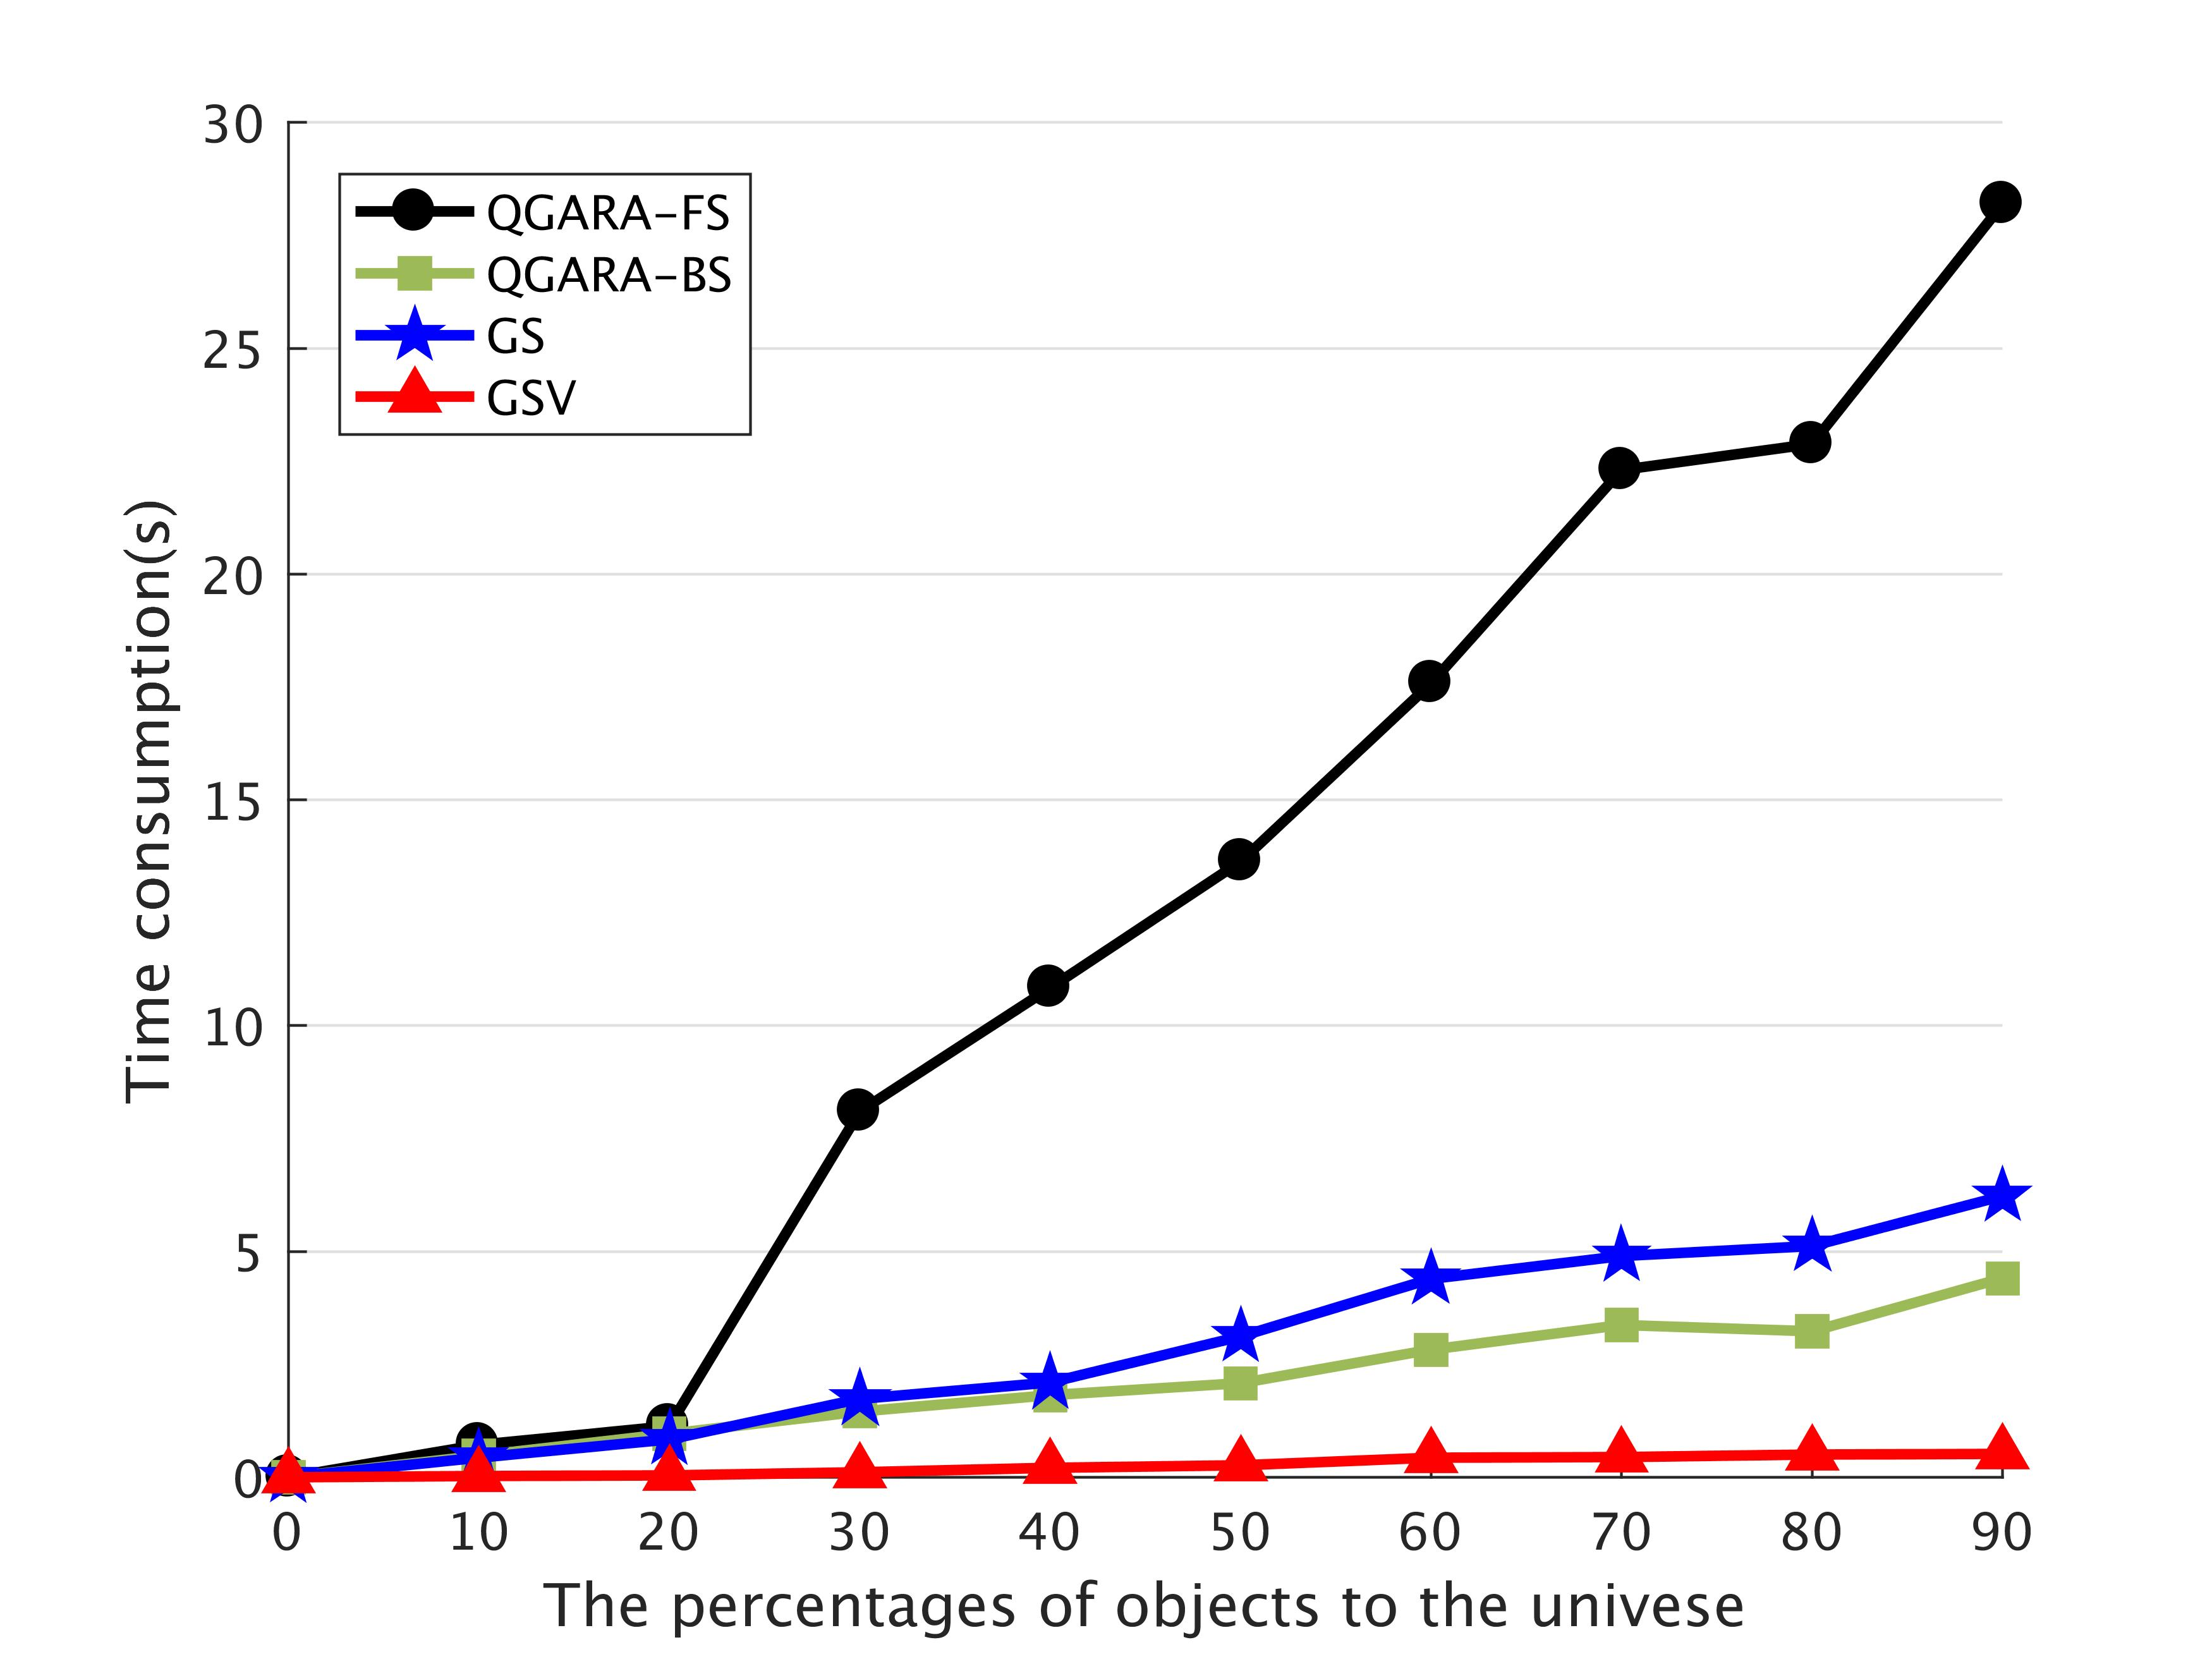
\includegraphics[width=5cm]{./Curve_universe/4_splice_pos.jpg} 
			}
			\subfigure[Dermatology]{
				\label{Fig.sub1.7}
				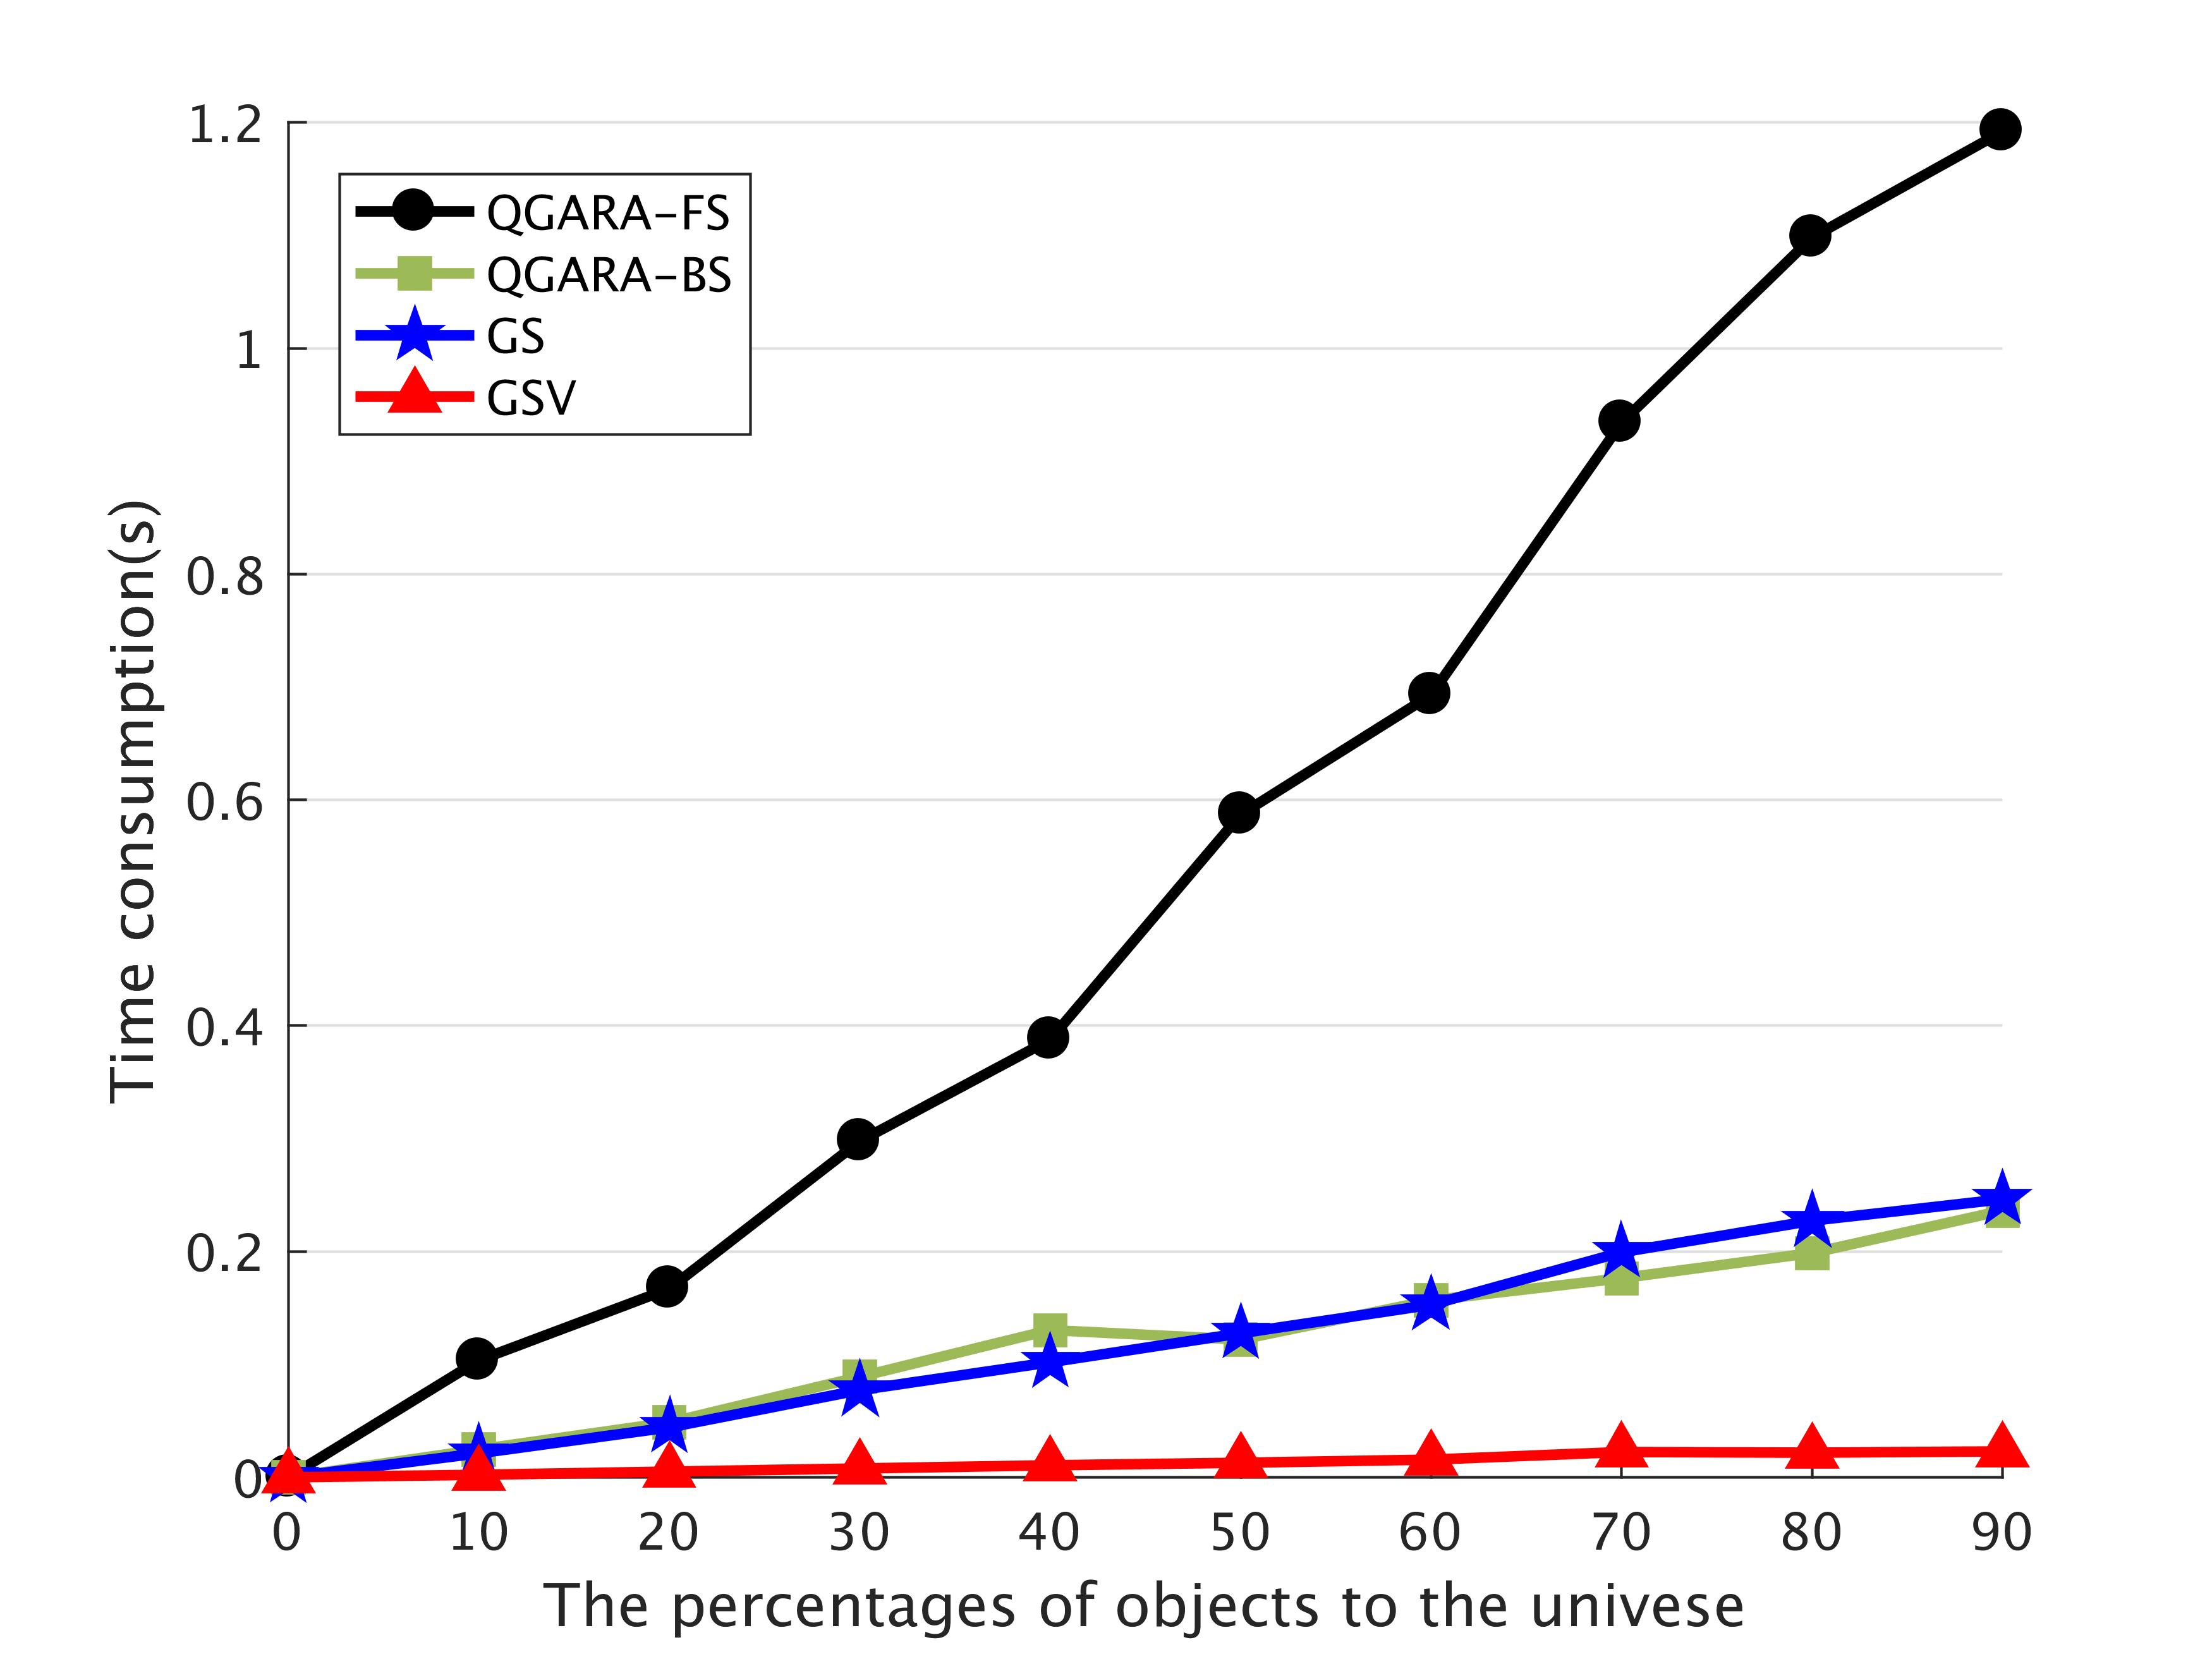
\includegraphics[width=5cm]{./Curve_universe/5_dermatology_pos.jpg} 
			}
			\subfigure[Wdbc]{
				\label{Fig.sub1.8}
				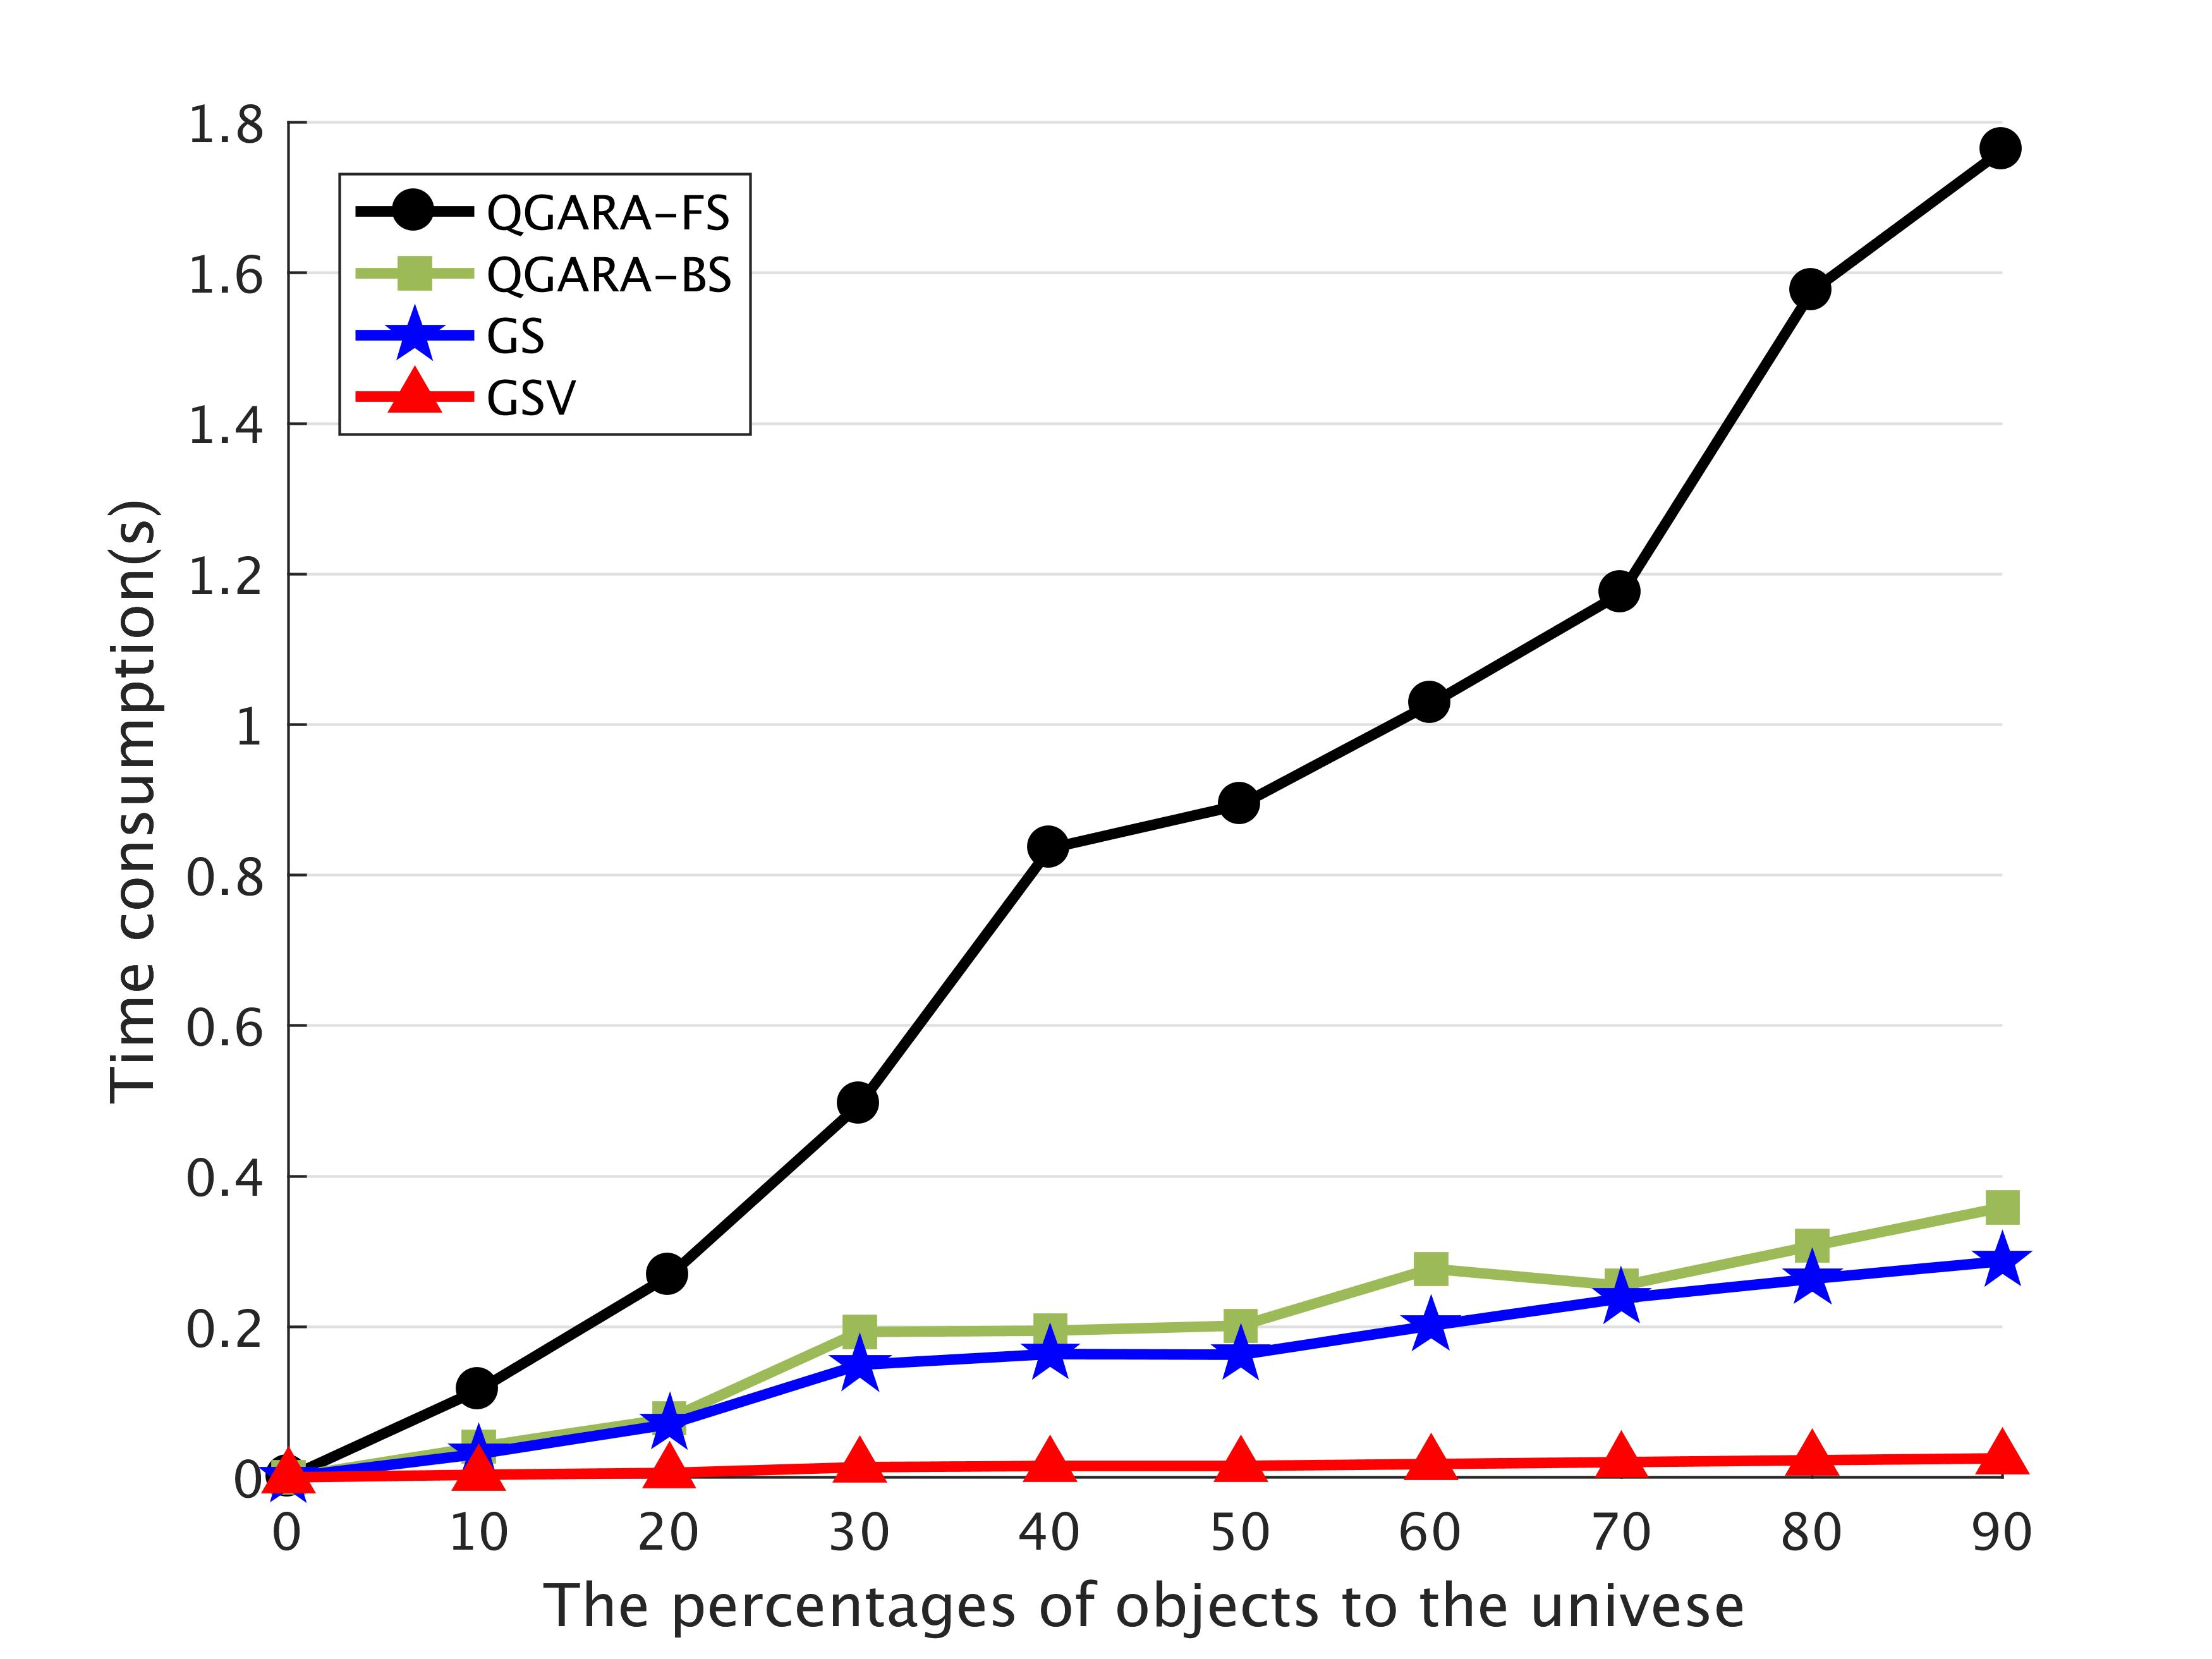
\includegraphics[width=5cm]{./Curve_universe/6_wdbc_pos.jpg} 
			}
	%	\end{figure}
	%	\begin{figure}[htbp]
			\subfigure[CNAE9]{
				\label{Fig.sub1.9}
				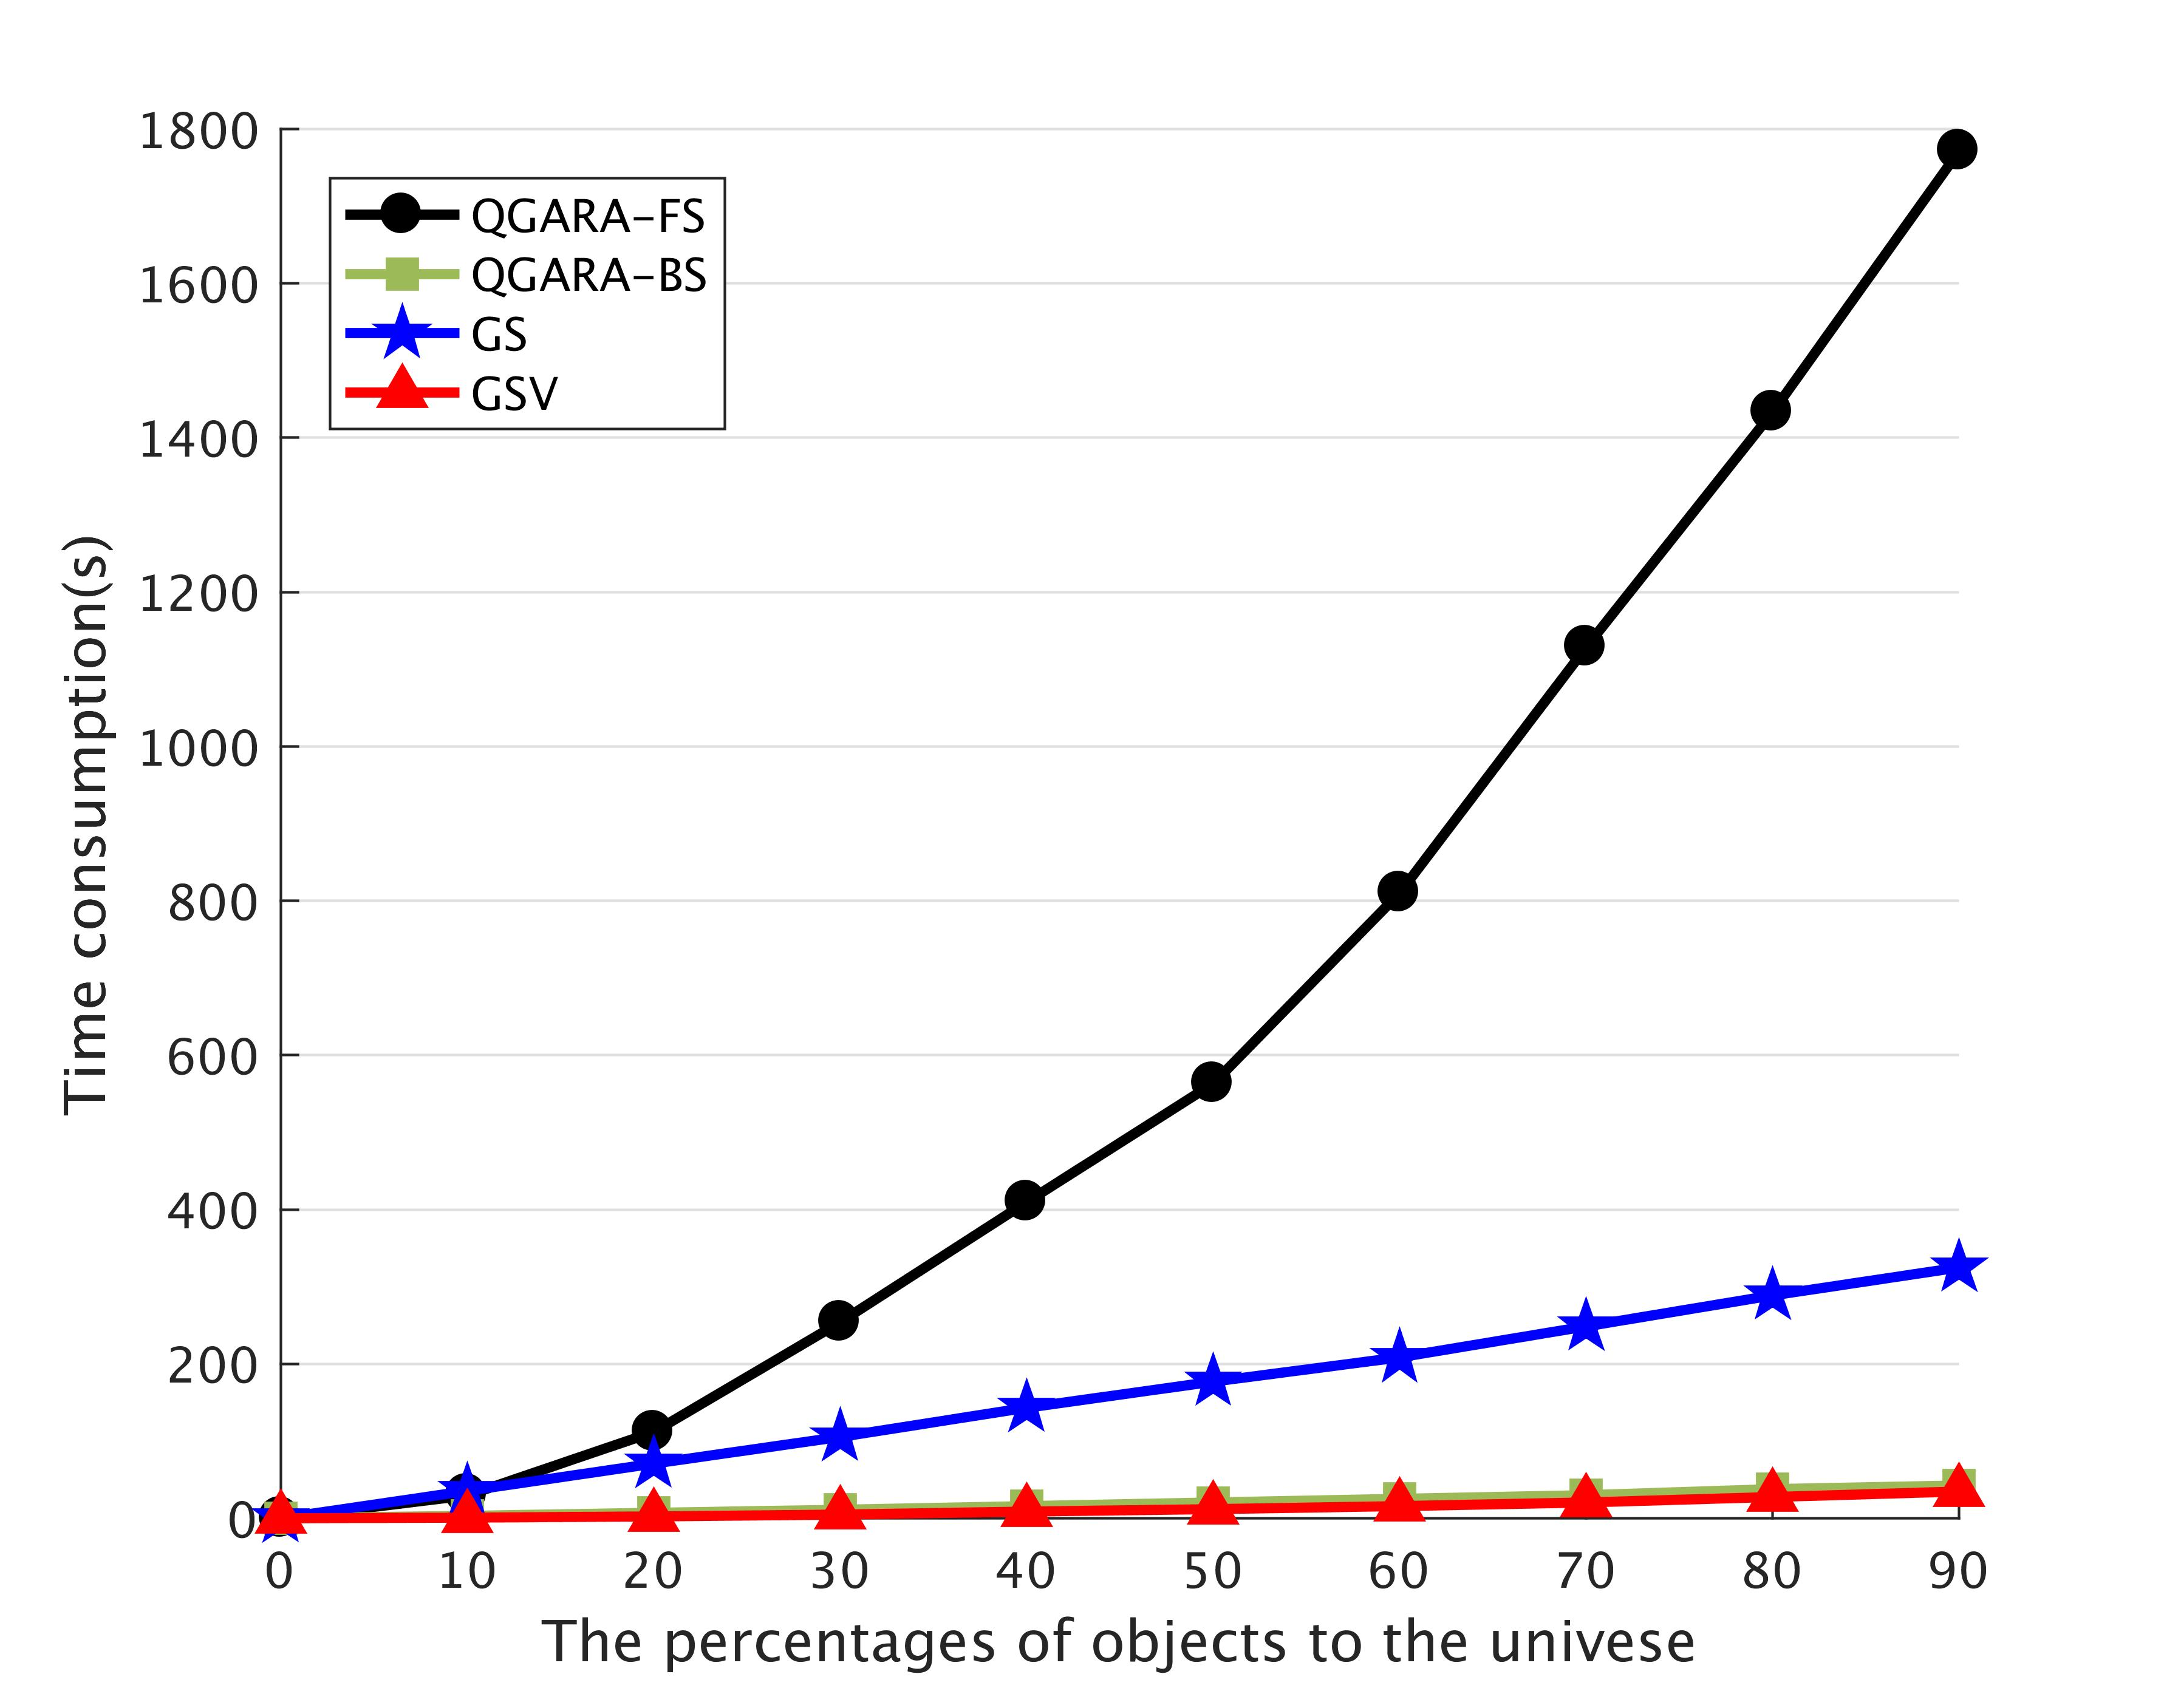
\includegraphics[width=5cm]{./Curve_universe/9.jpg} 
			}
%			\subfigure[Semeion]{
%				\label{Fig.sub1.10}
%				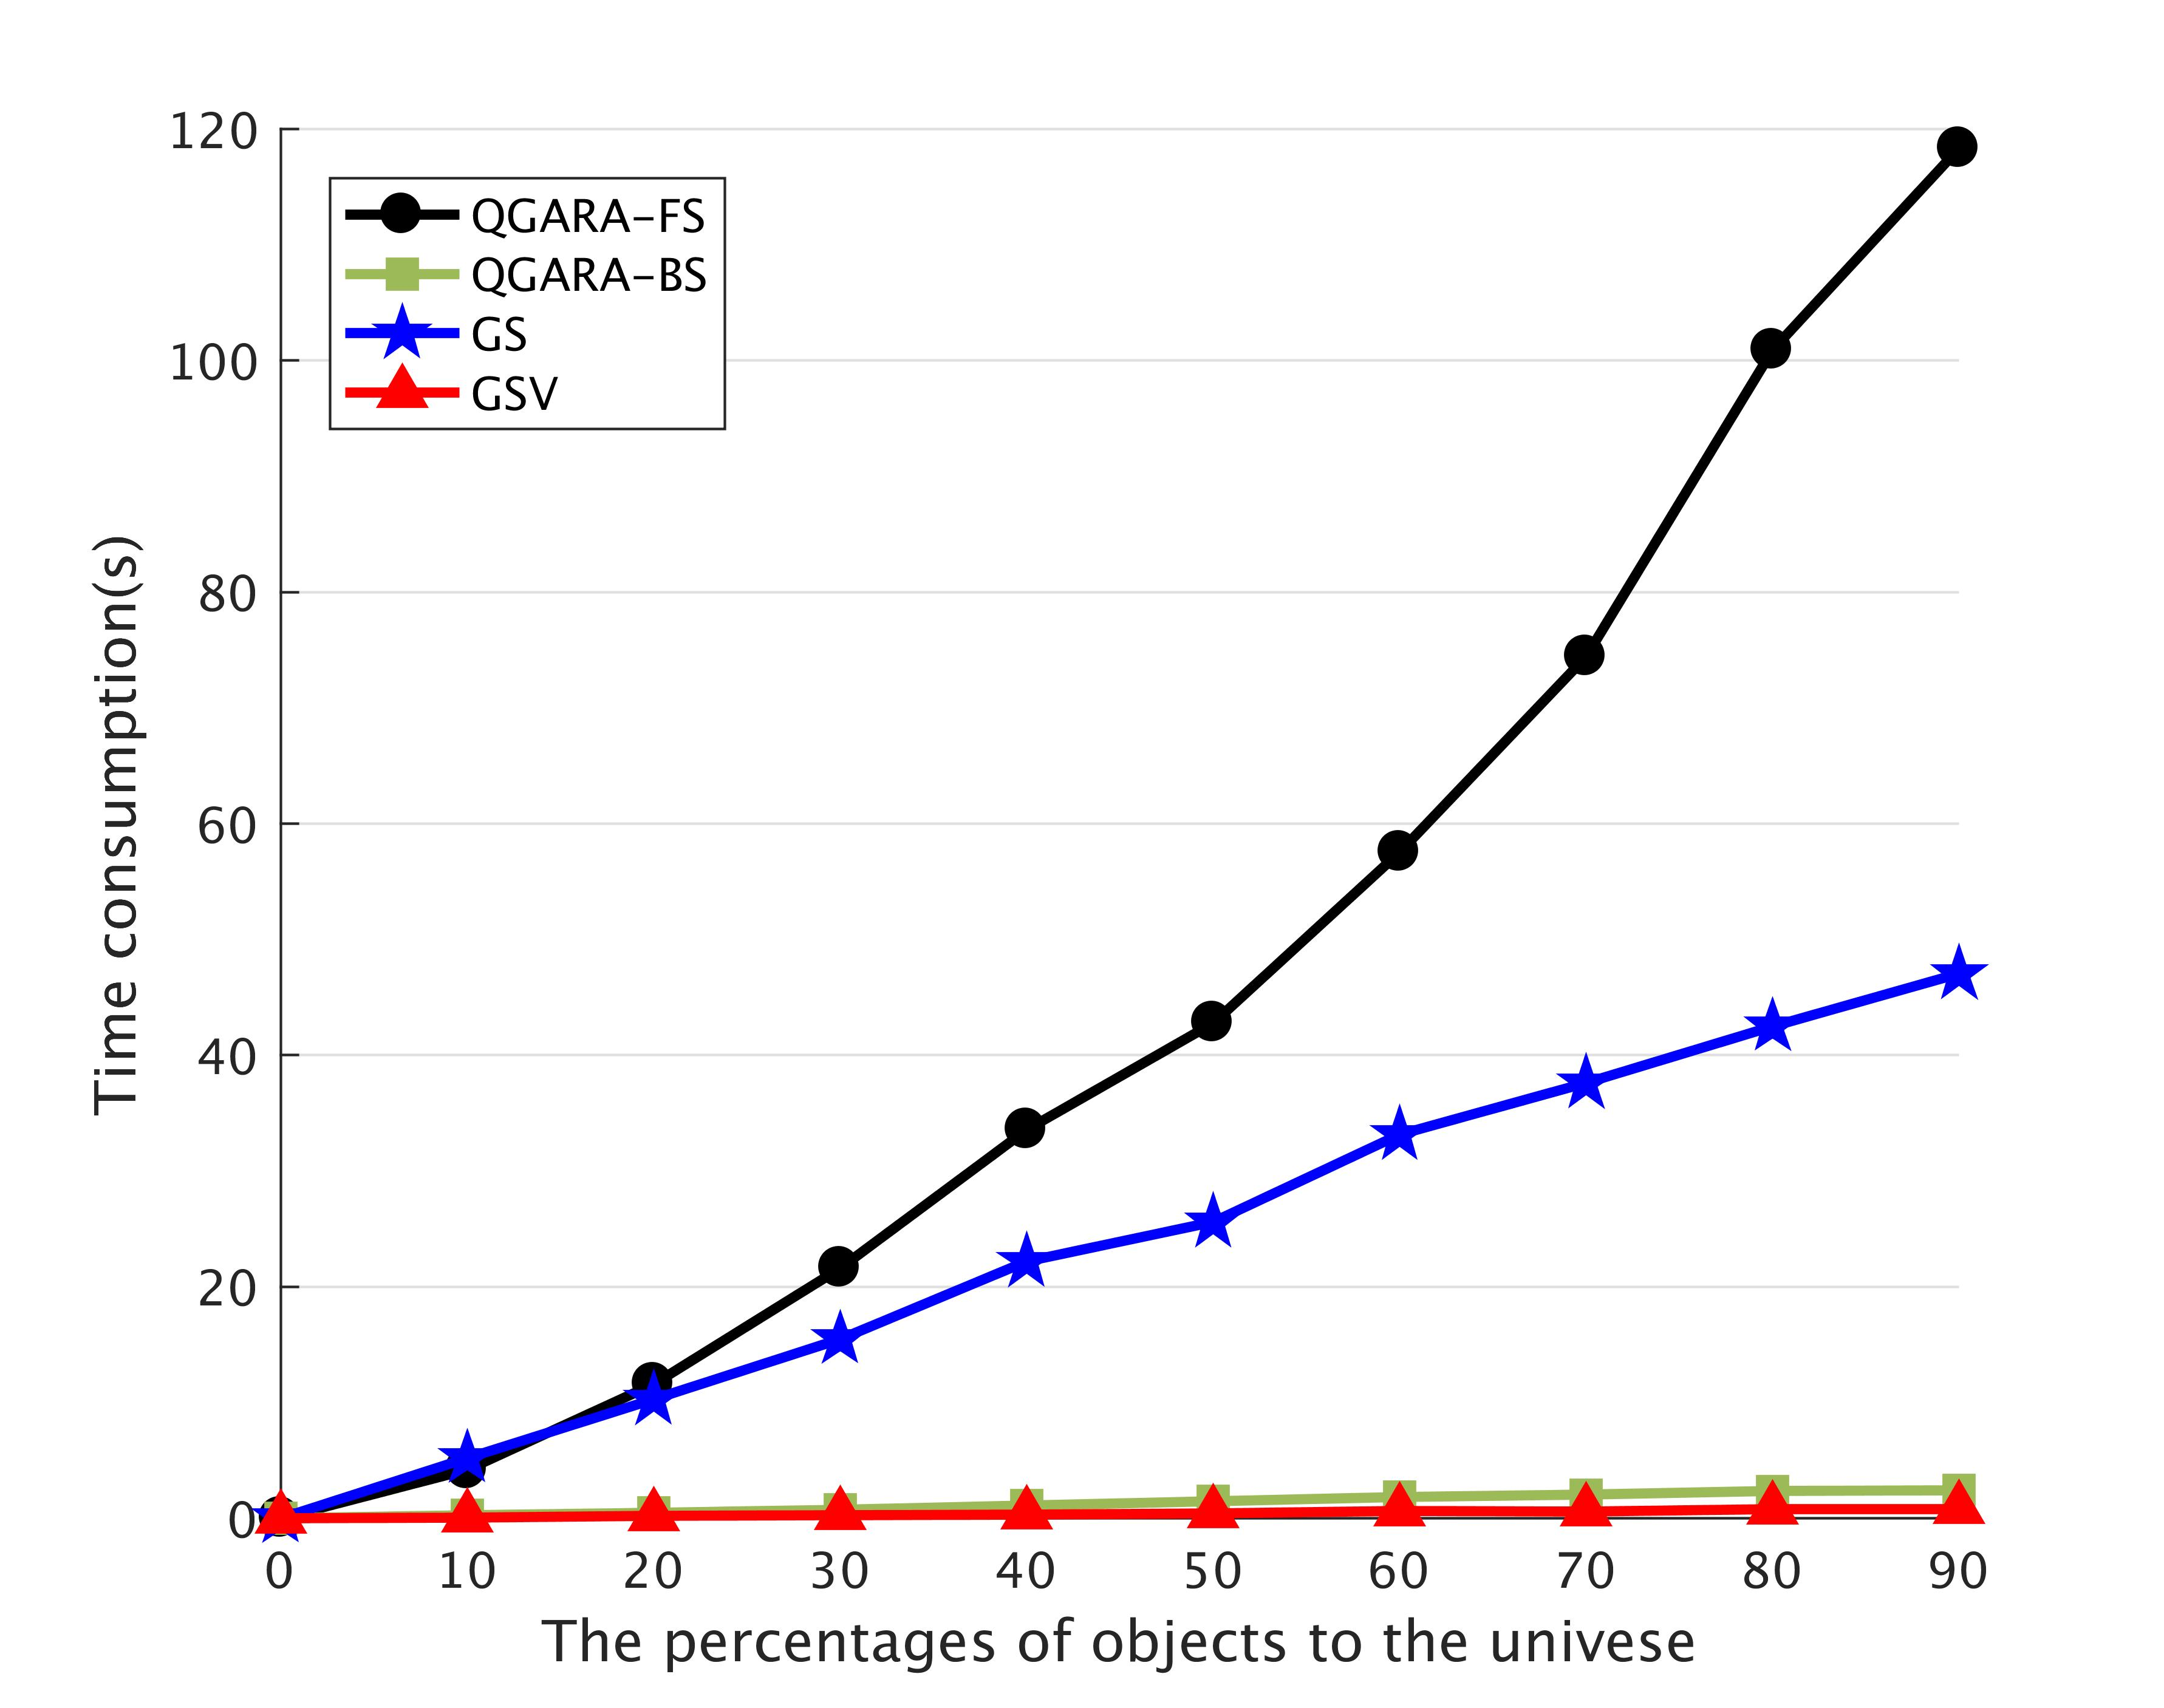
\includegraphics[width=5cm]{./Curve_universe/10.jpg} 
%			}
			\subfigure[DNA]{
				\label{Fig.sub1.11}
				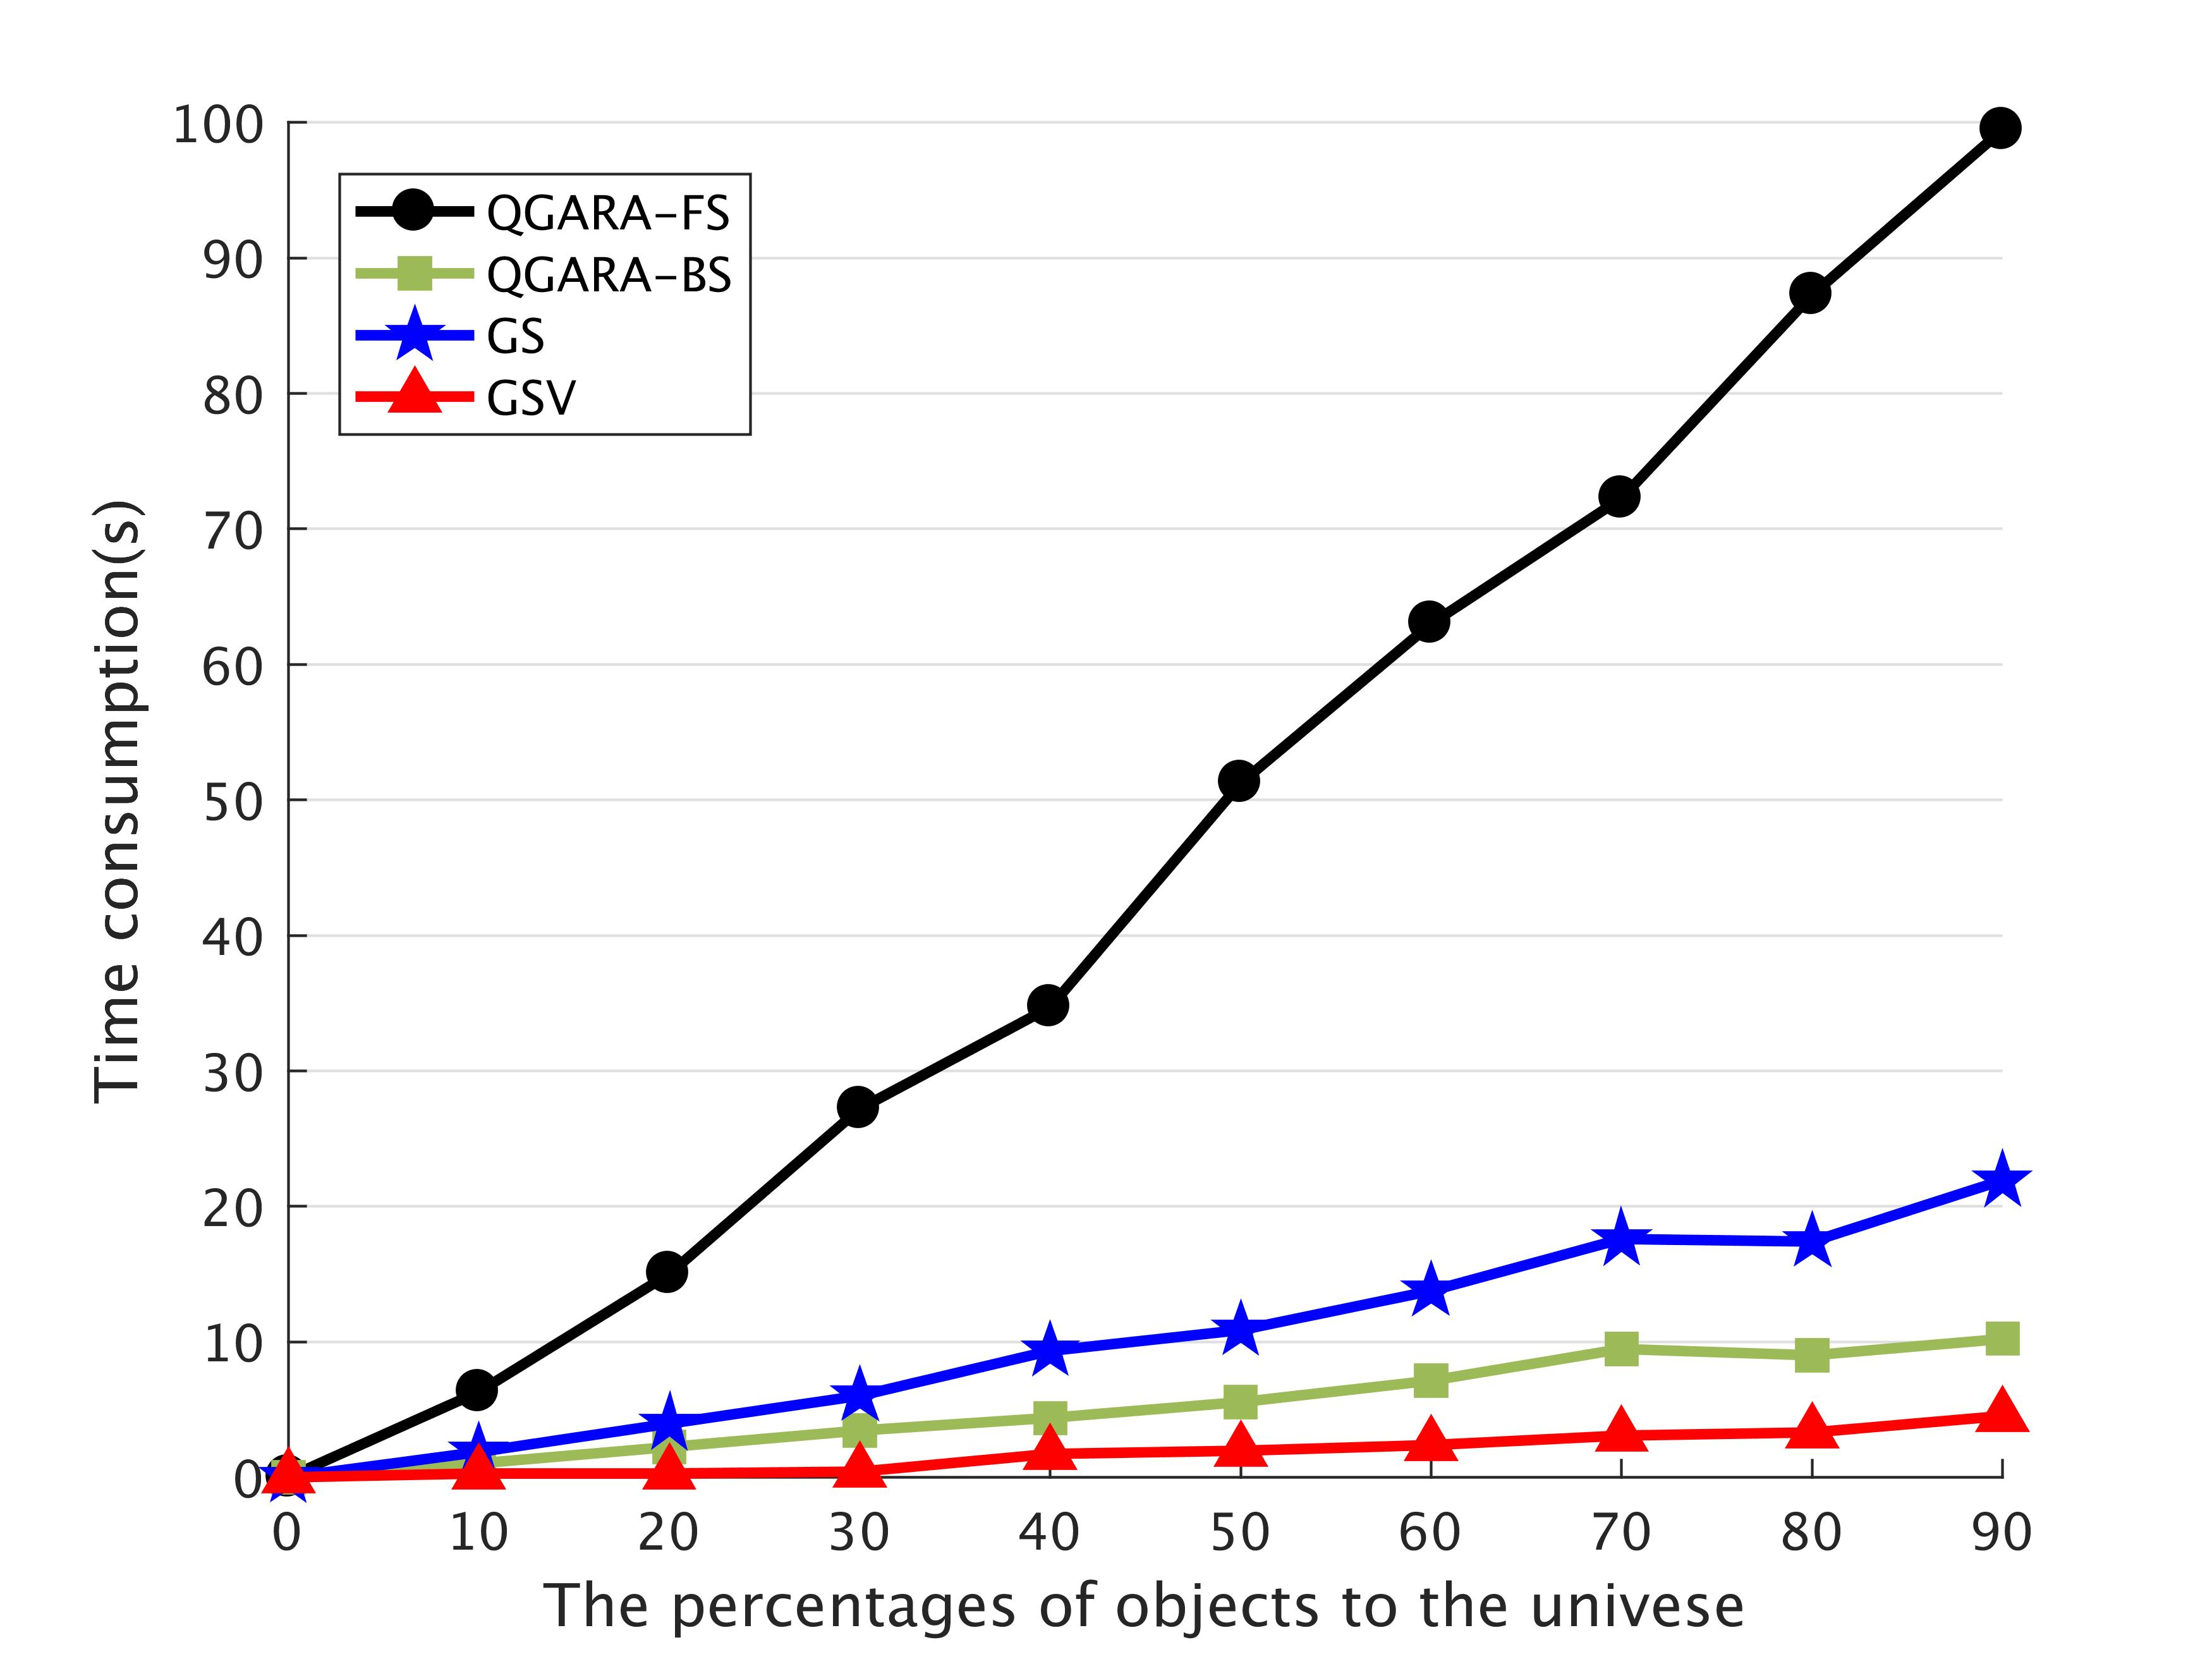
\includegraphics[width=5cm]{./Curve_universe/9_DNA_pos.jpg} 
			}
			\subfigure[Connect4]{
				\label{Fig.sub1.12}
				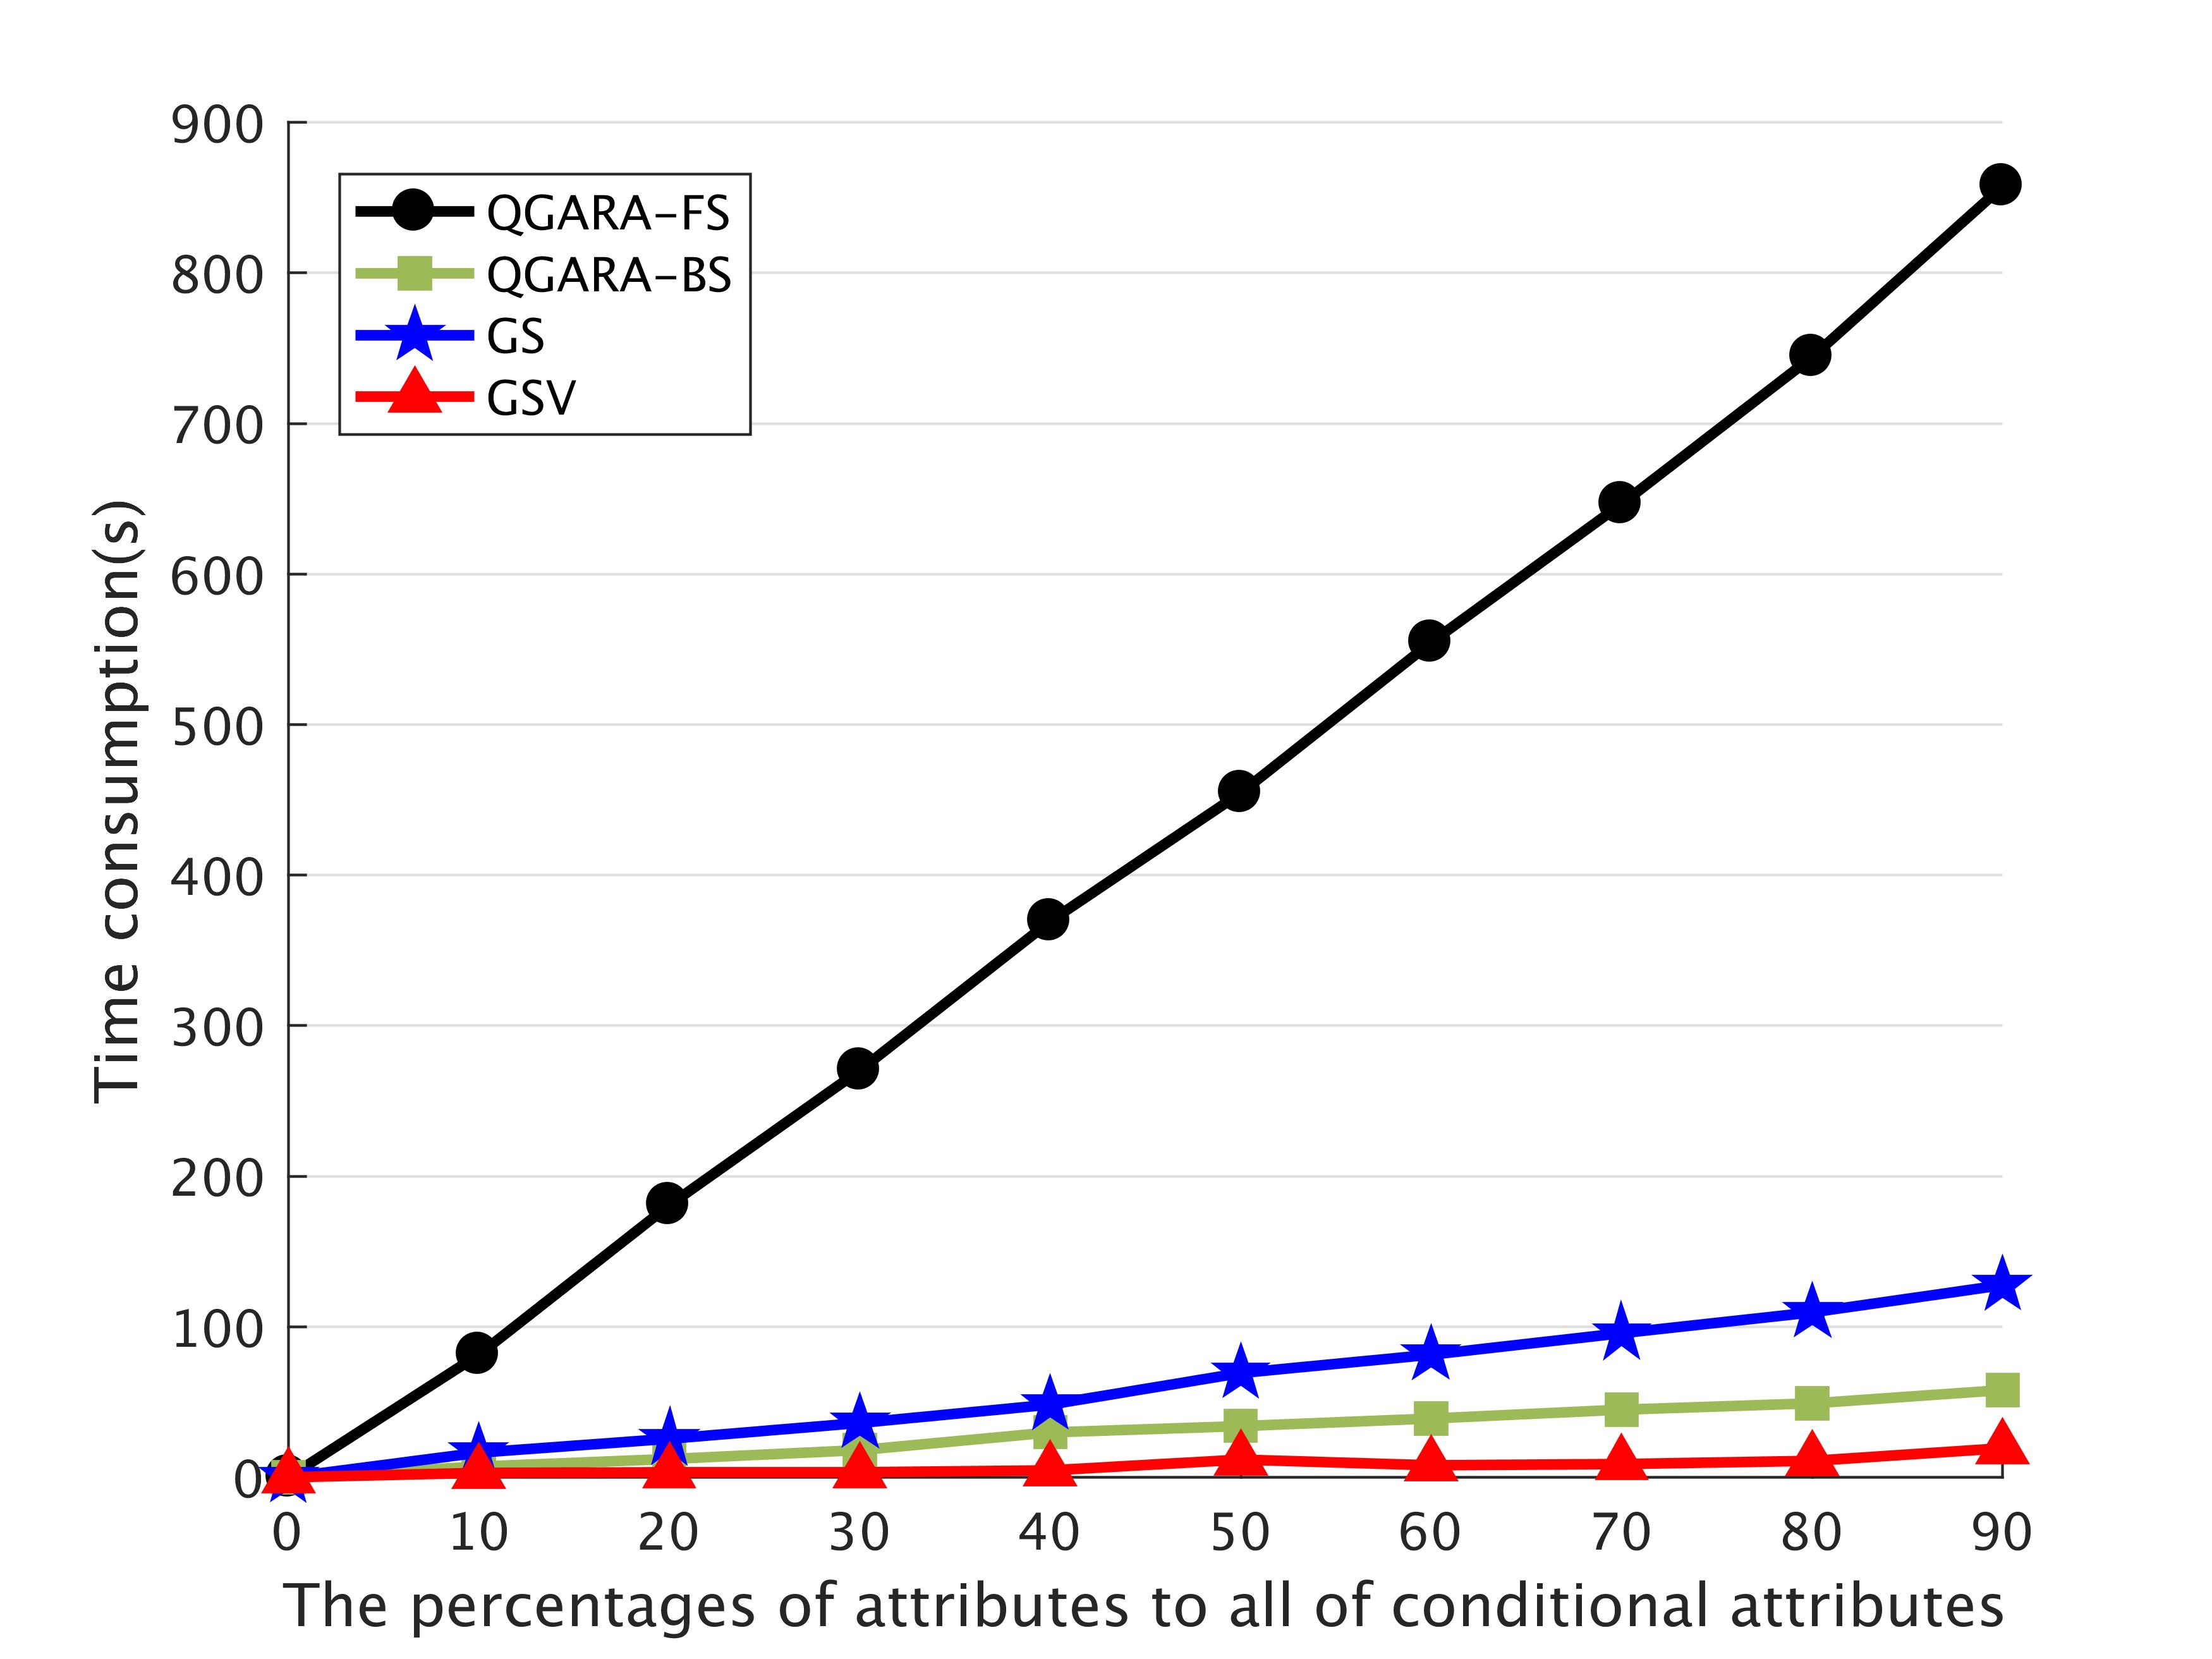
\includegraphics[width=5cm]{./Curve_universe/10_cnnect4_pos.jpg} 
			}
			\caption{The time of general reduction algorithms versus the size of objects} 
			\label{TimeIncreaseObjects}
		\end{figure}
		
		\begin{figure}[htbp]
			\centering 
			\subfigure[Mushroom]{
				\label{Fig.sub2.2}
				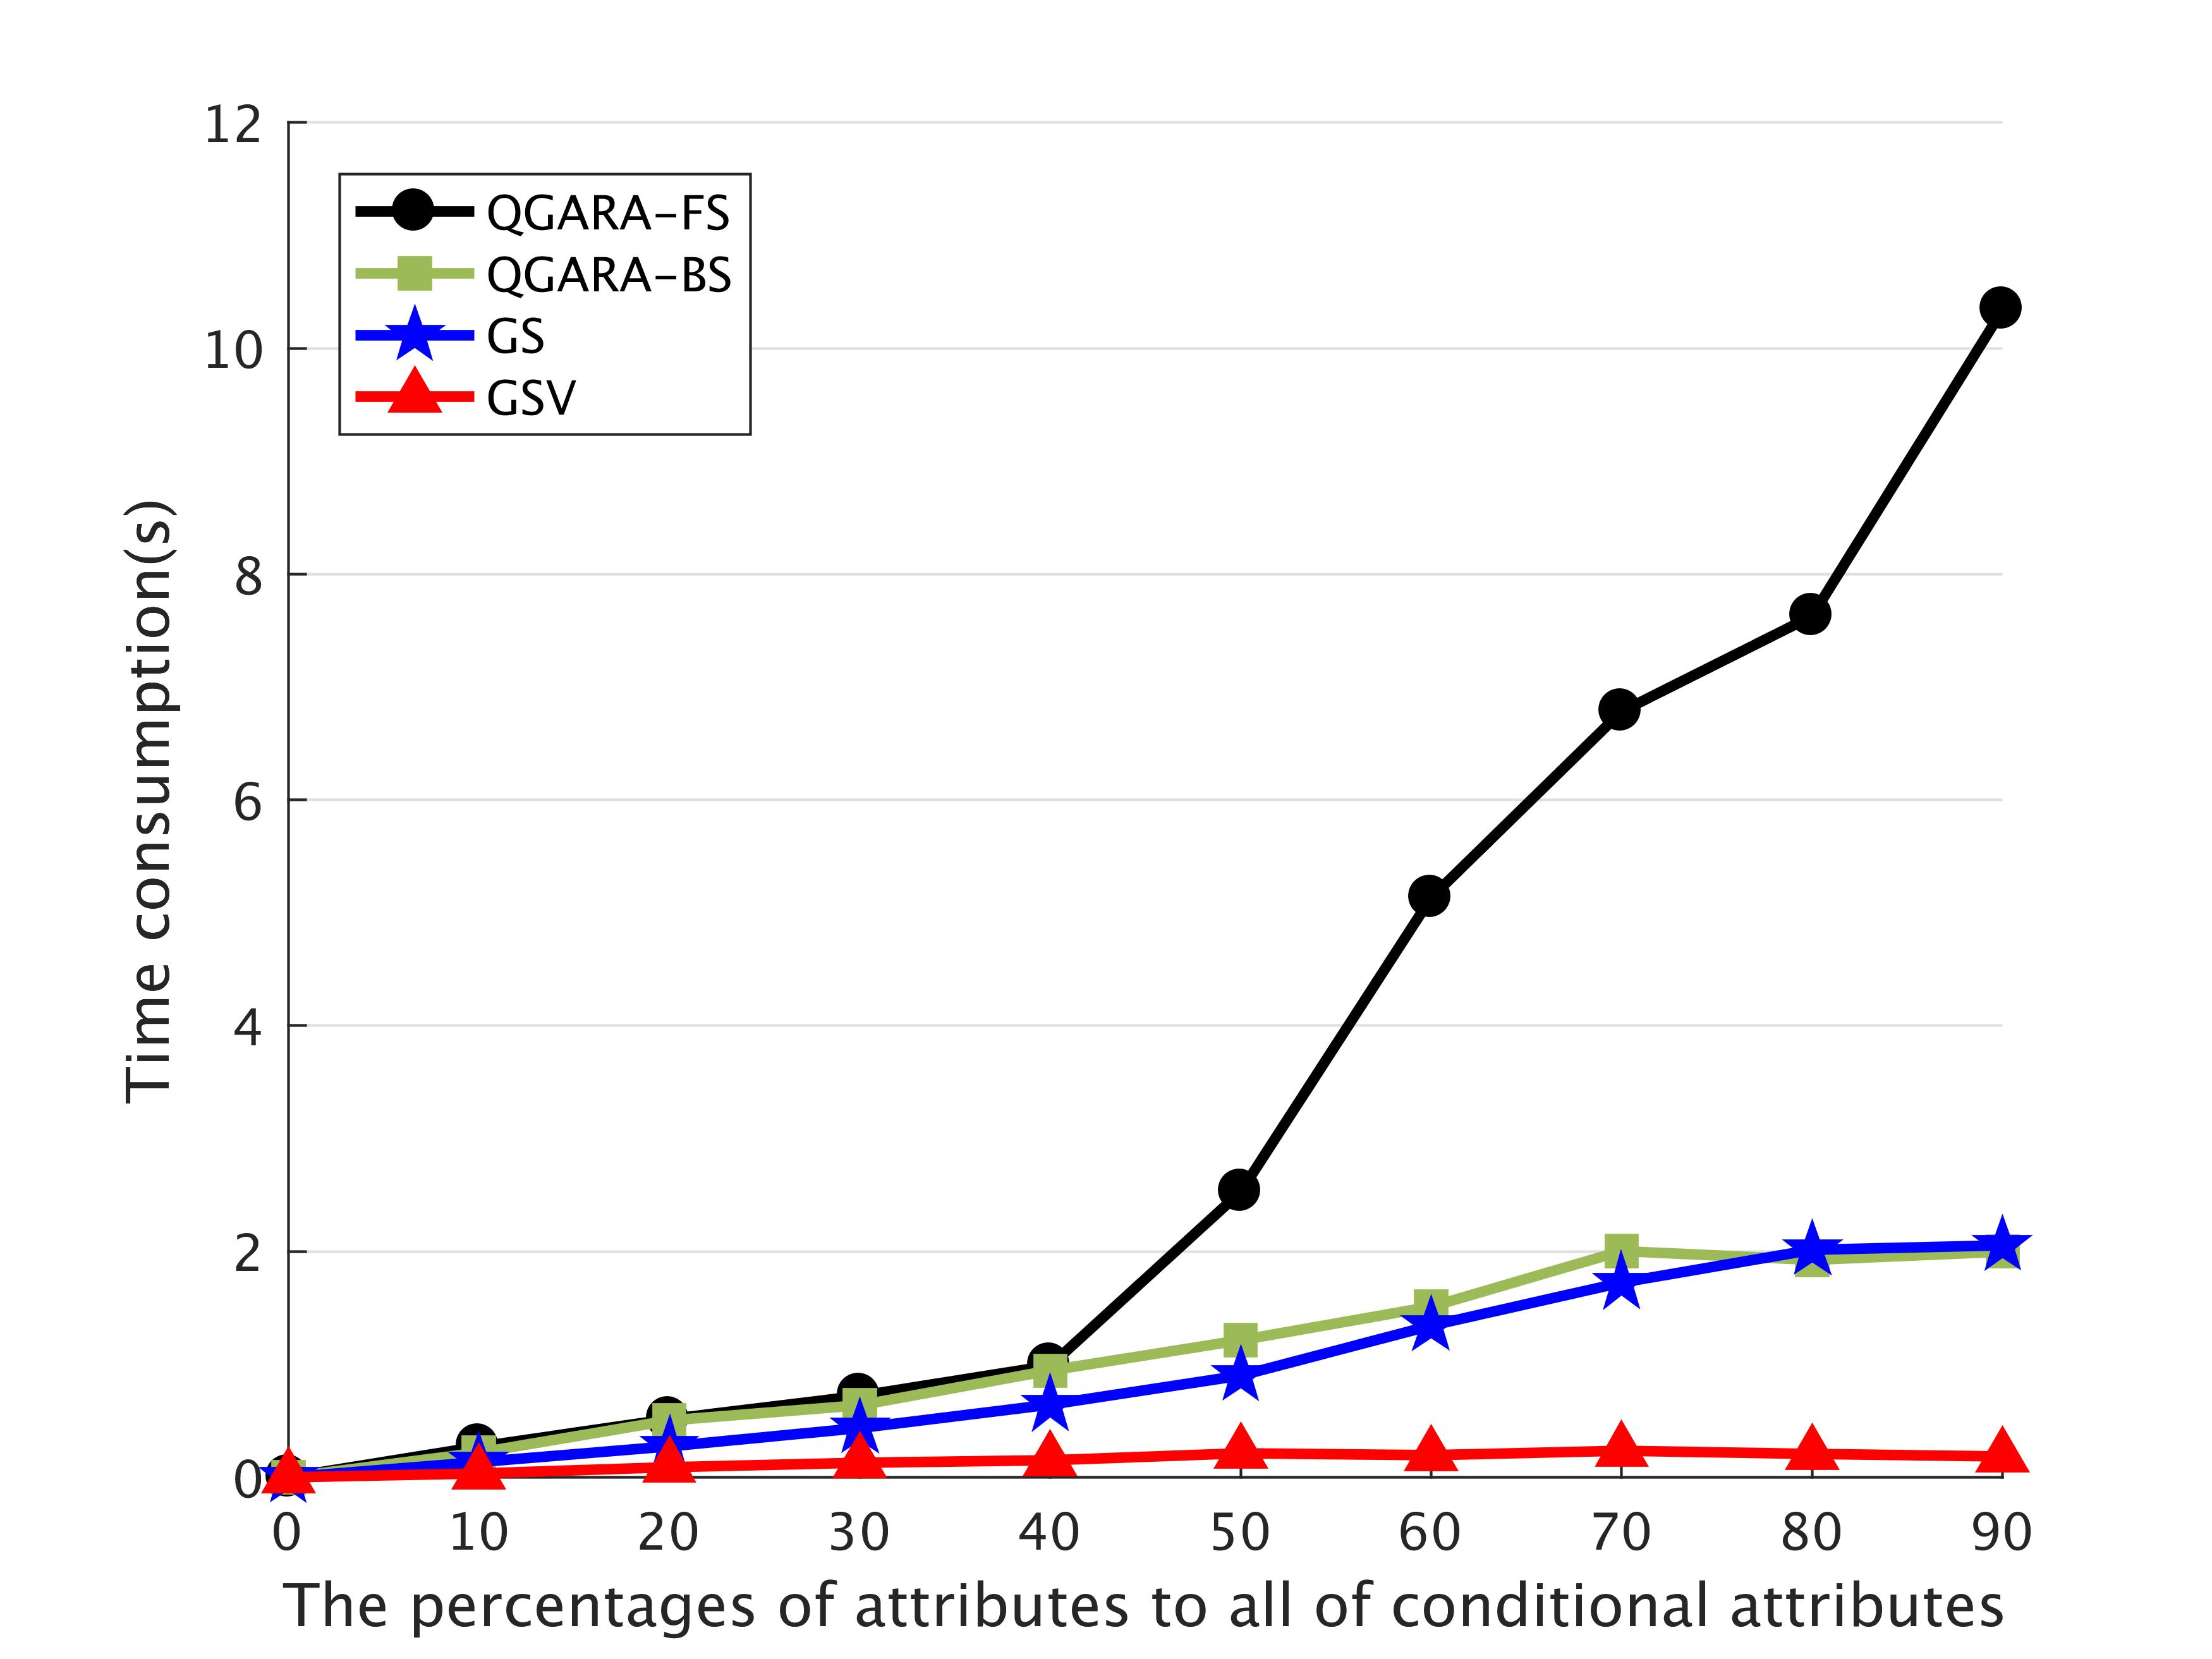
\includegraphics[width=5cm]{./Curve_attributes/1_mushroom_pos.jpg} 
			}
			\subfigure[Tic]{
				\label{Fig.sub2.3}
				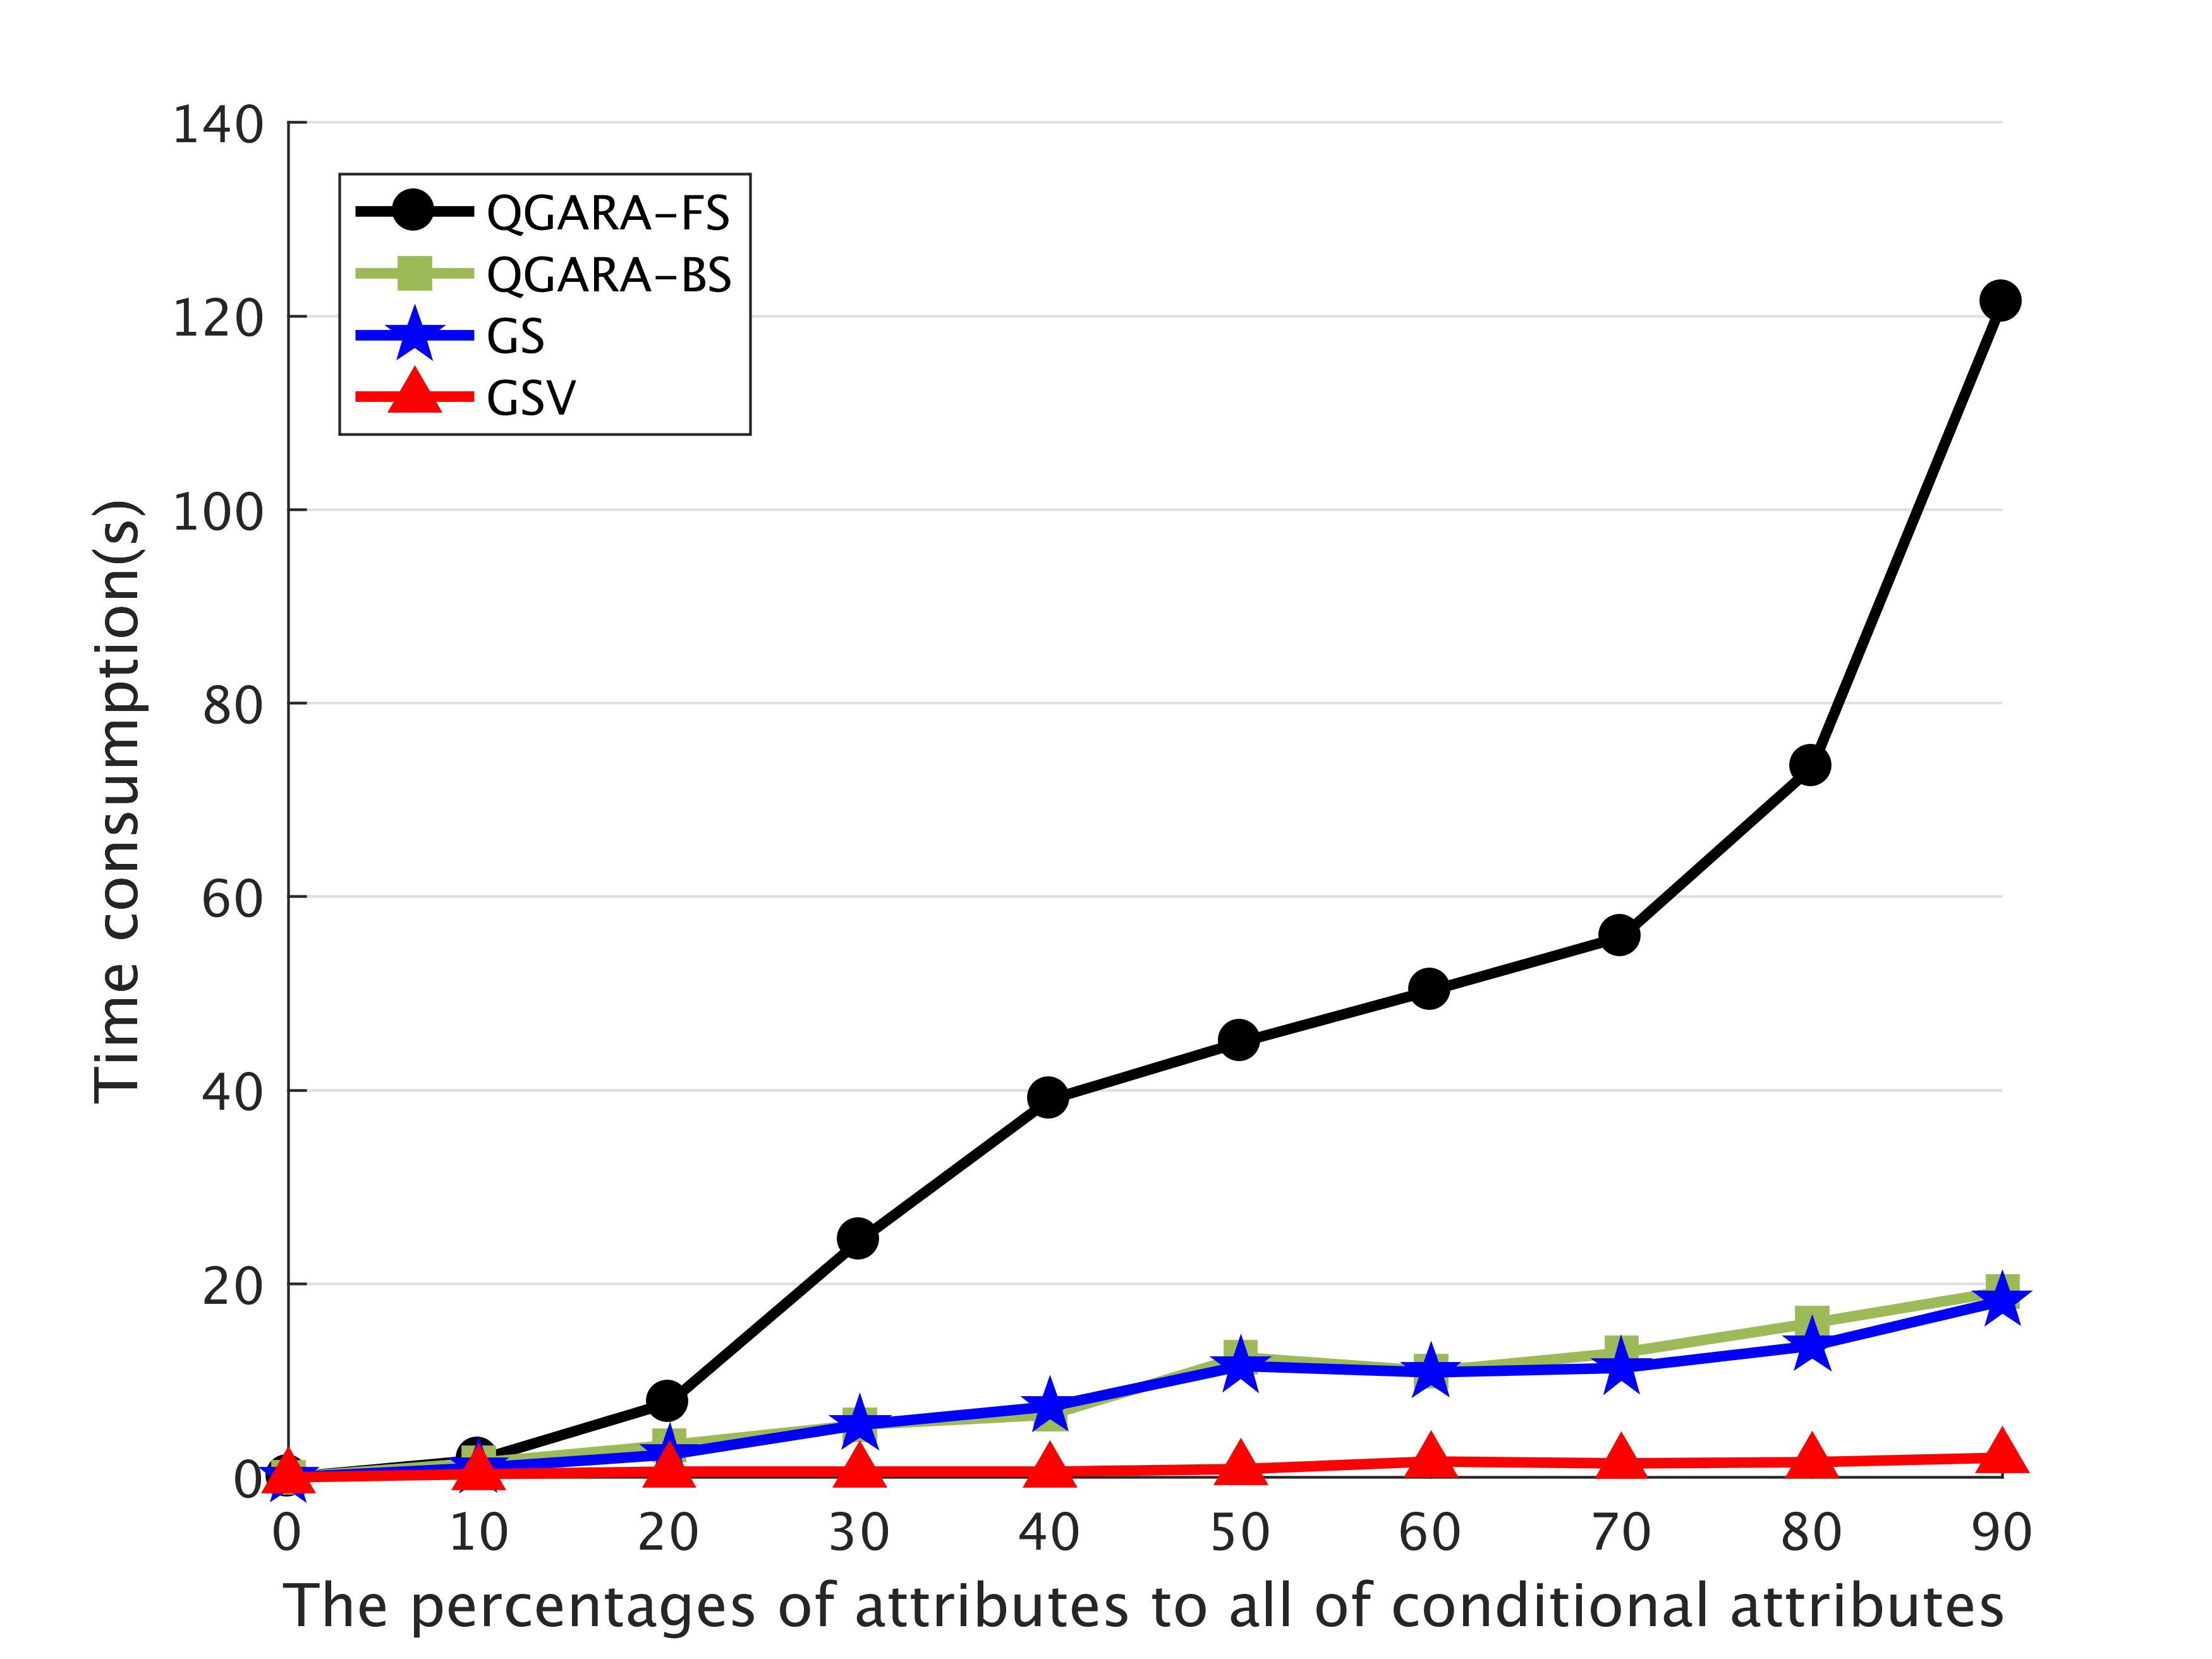
\includegraphics[width=5cm]{./Curve_attributes/2_tic_pos.jpg} 
			}
			\subfigure[Segmentation]{
				\label{Fig.sub2.4}
				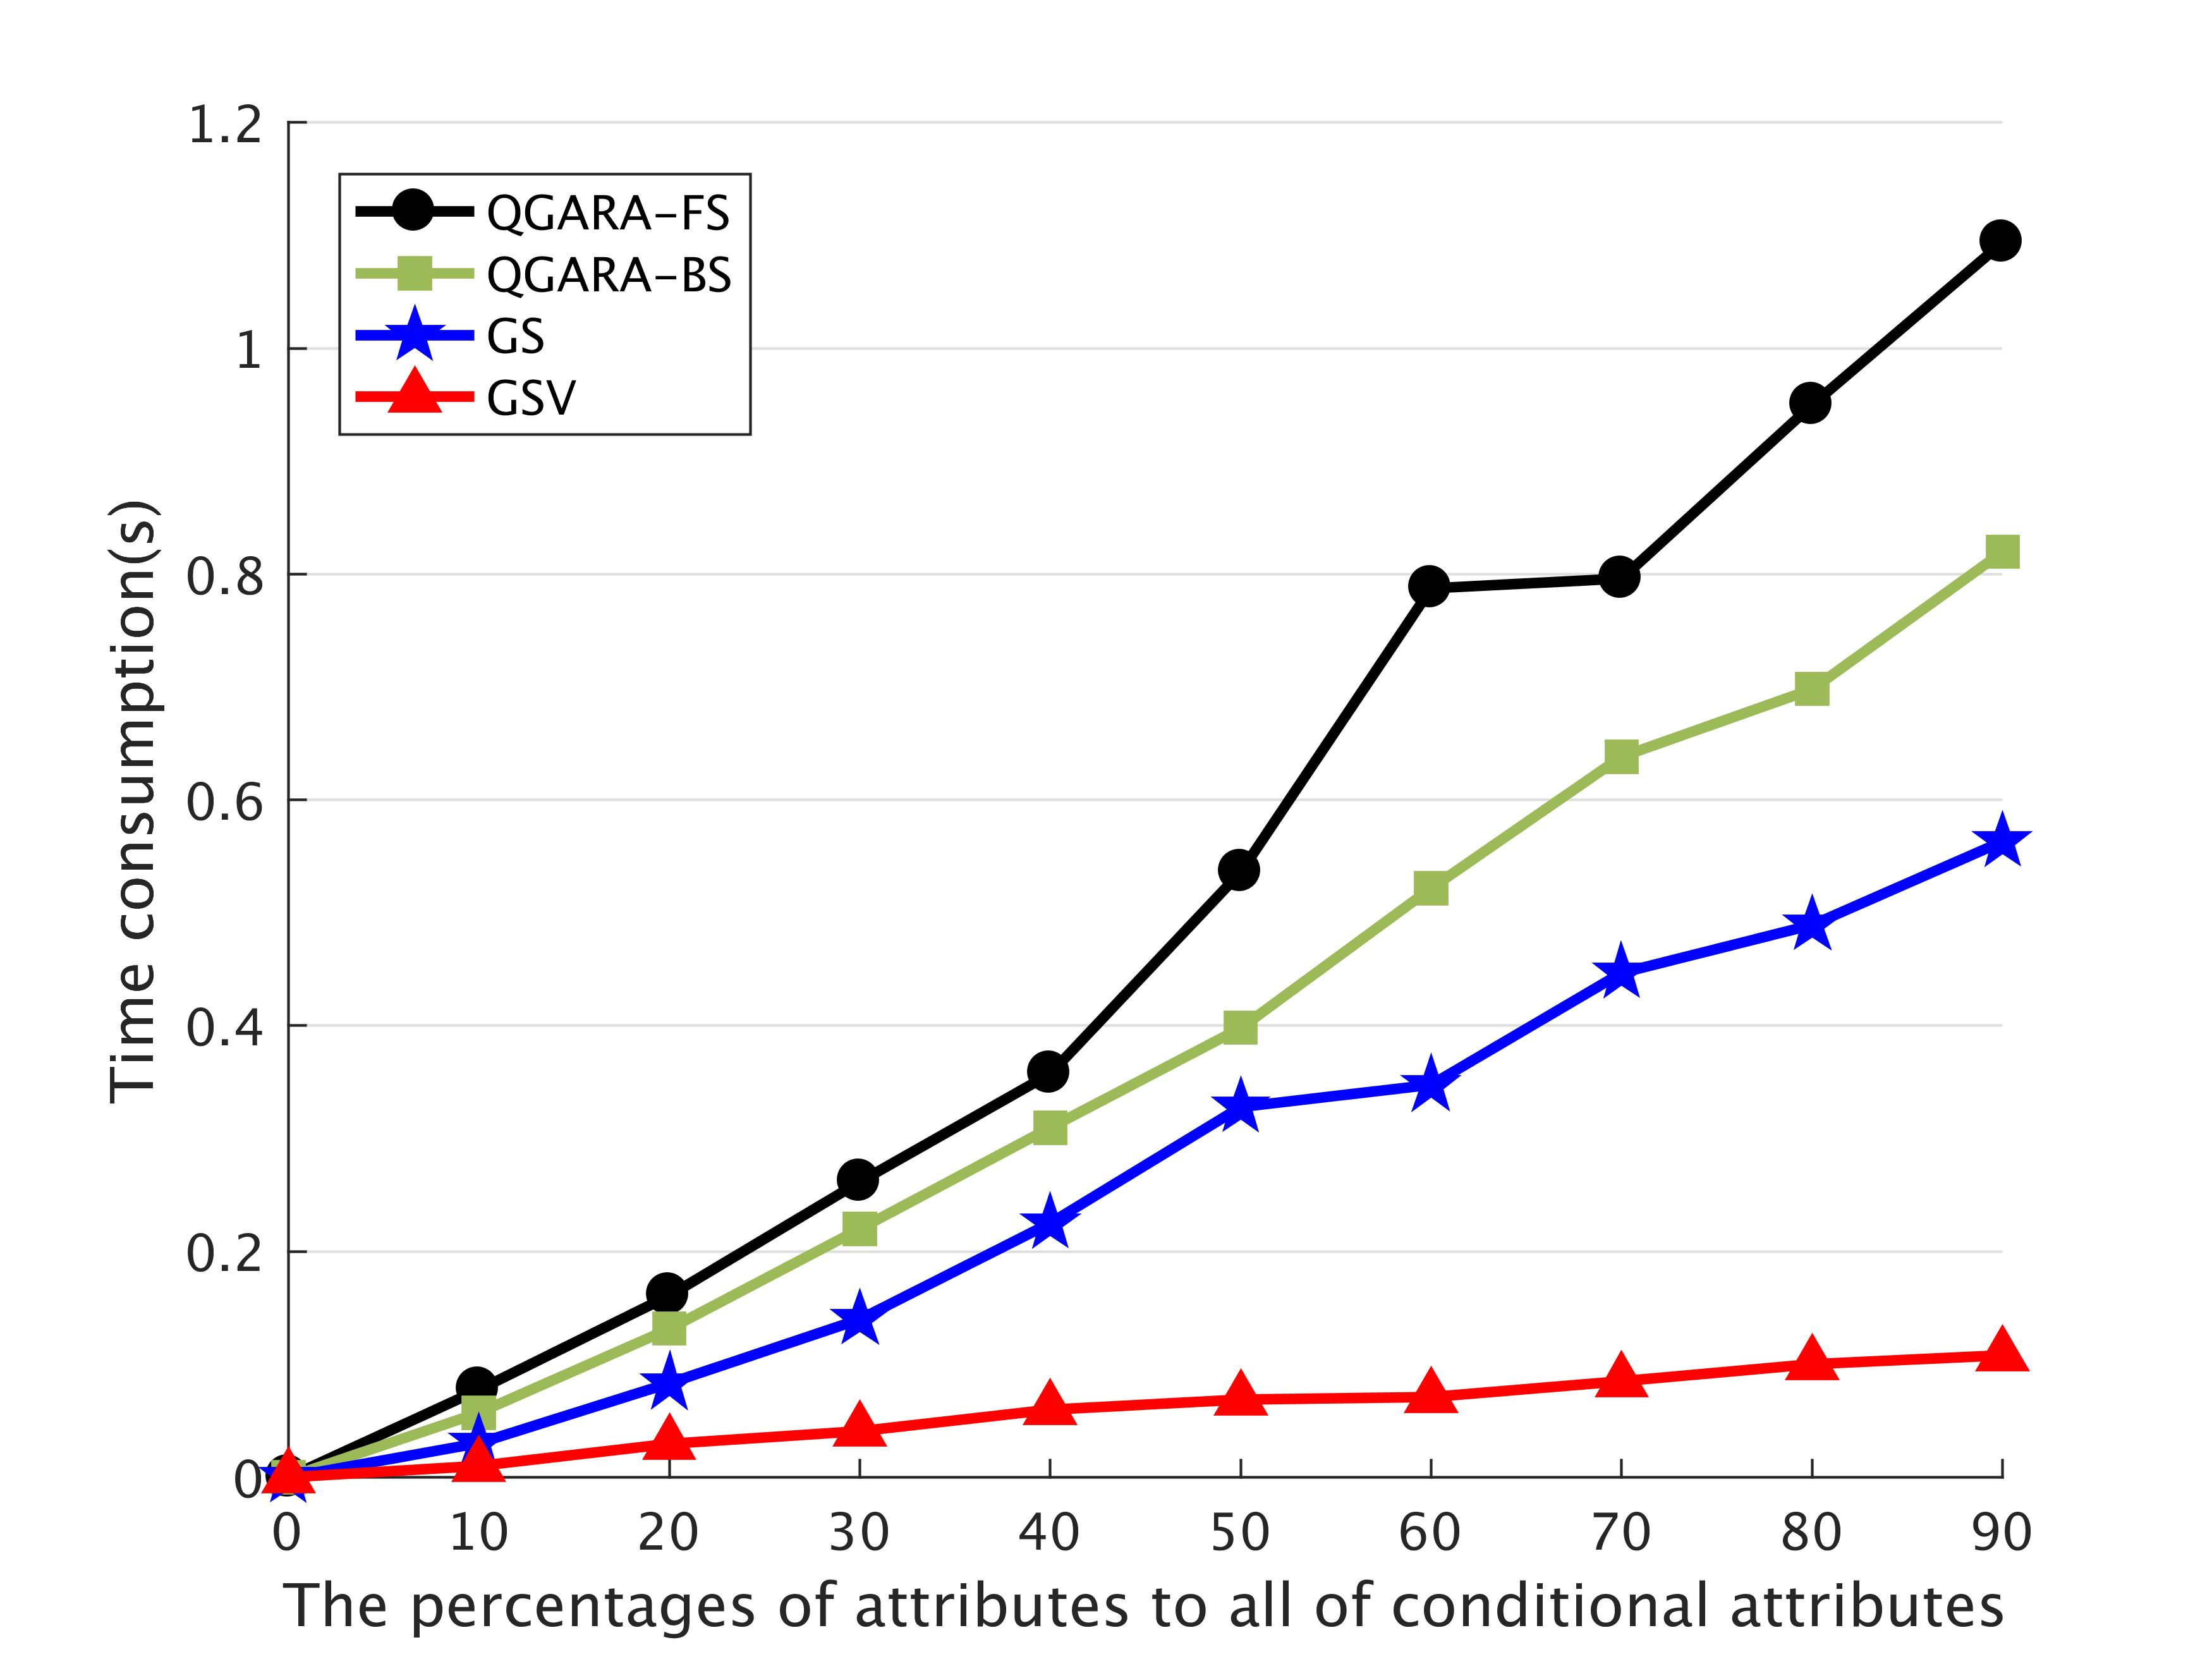
\includegraphics[width=5cm]{./Curve_attributes/3_seg_pos.jpg} 
			}
			\subfigure[Splice]{
				\label{Fig.sub2.6}
				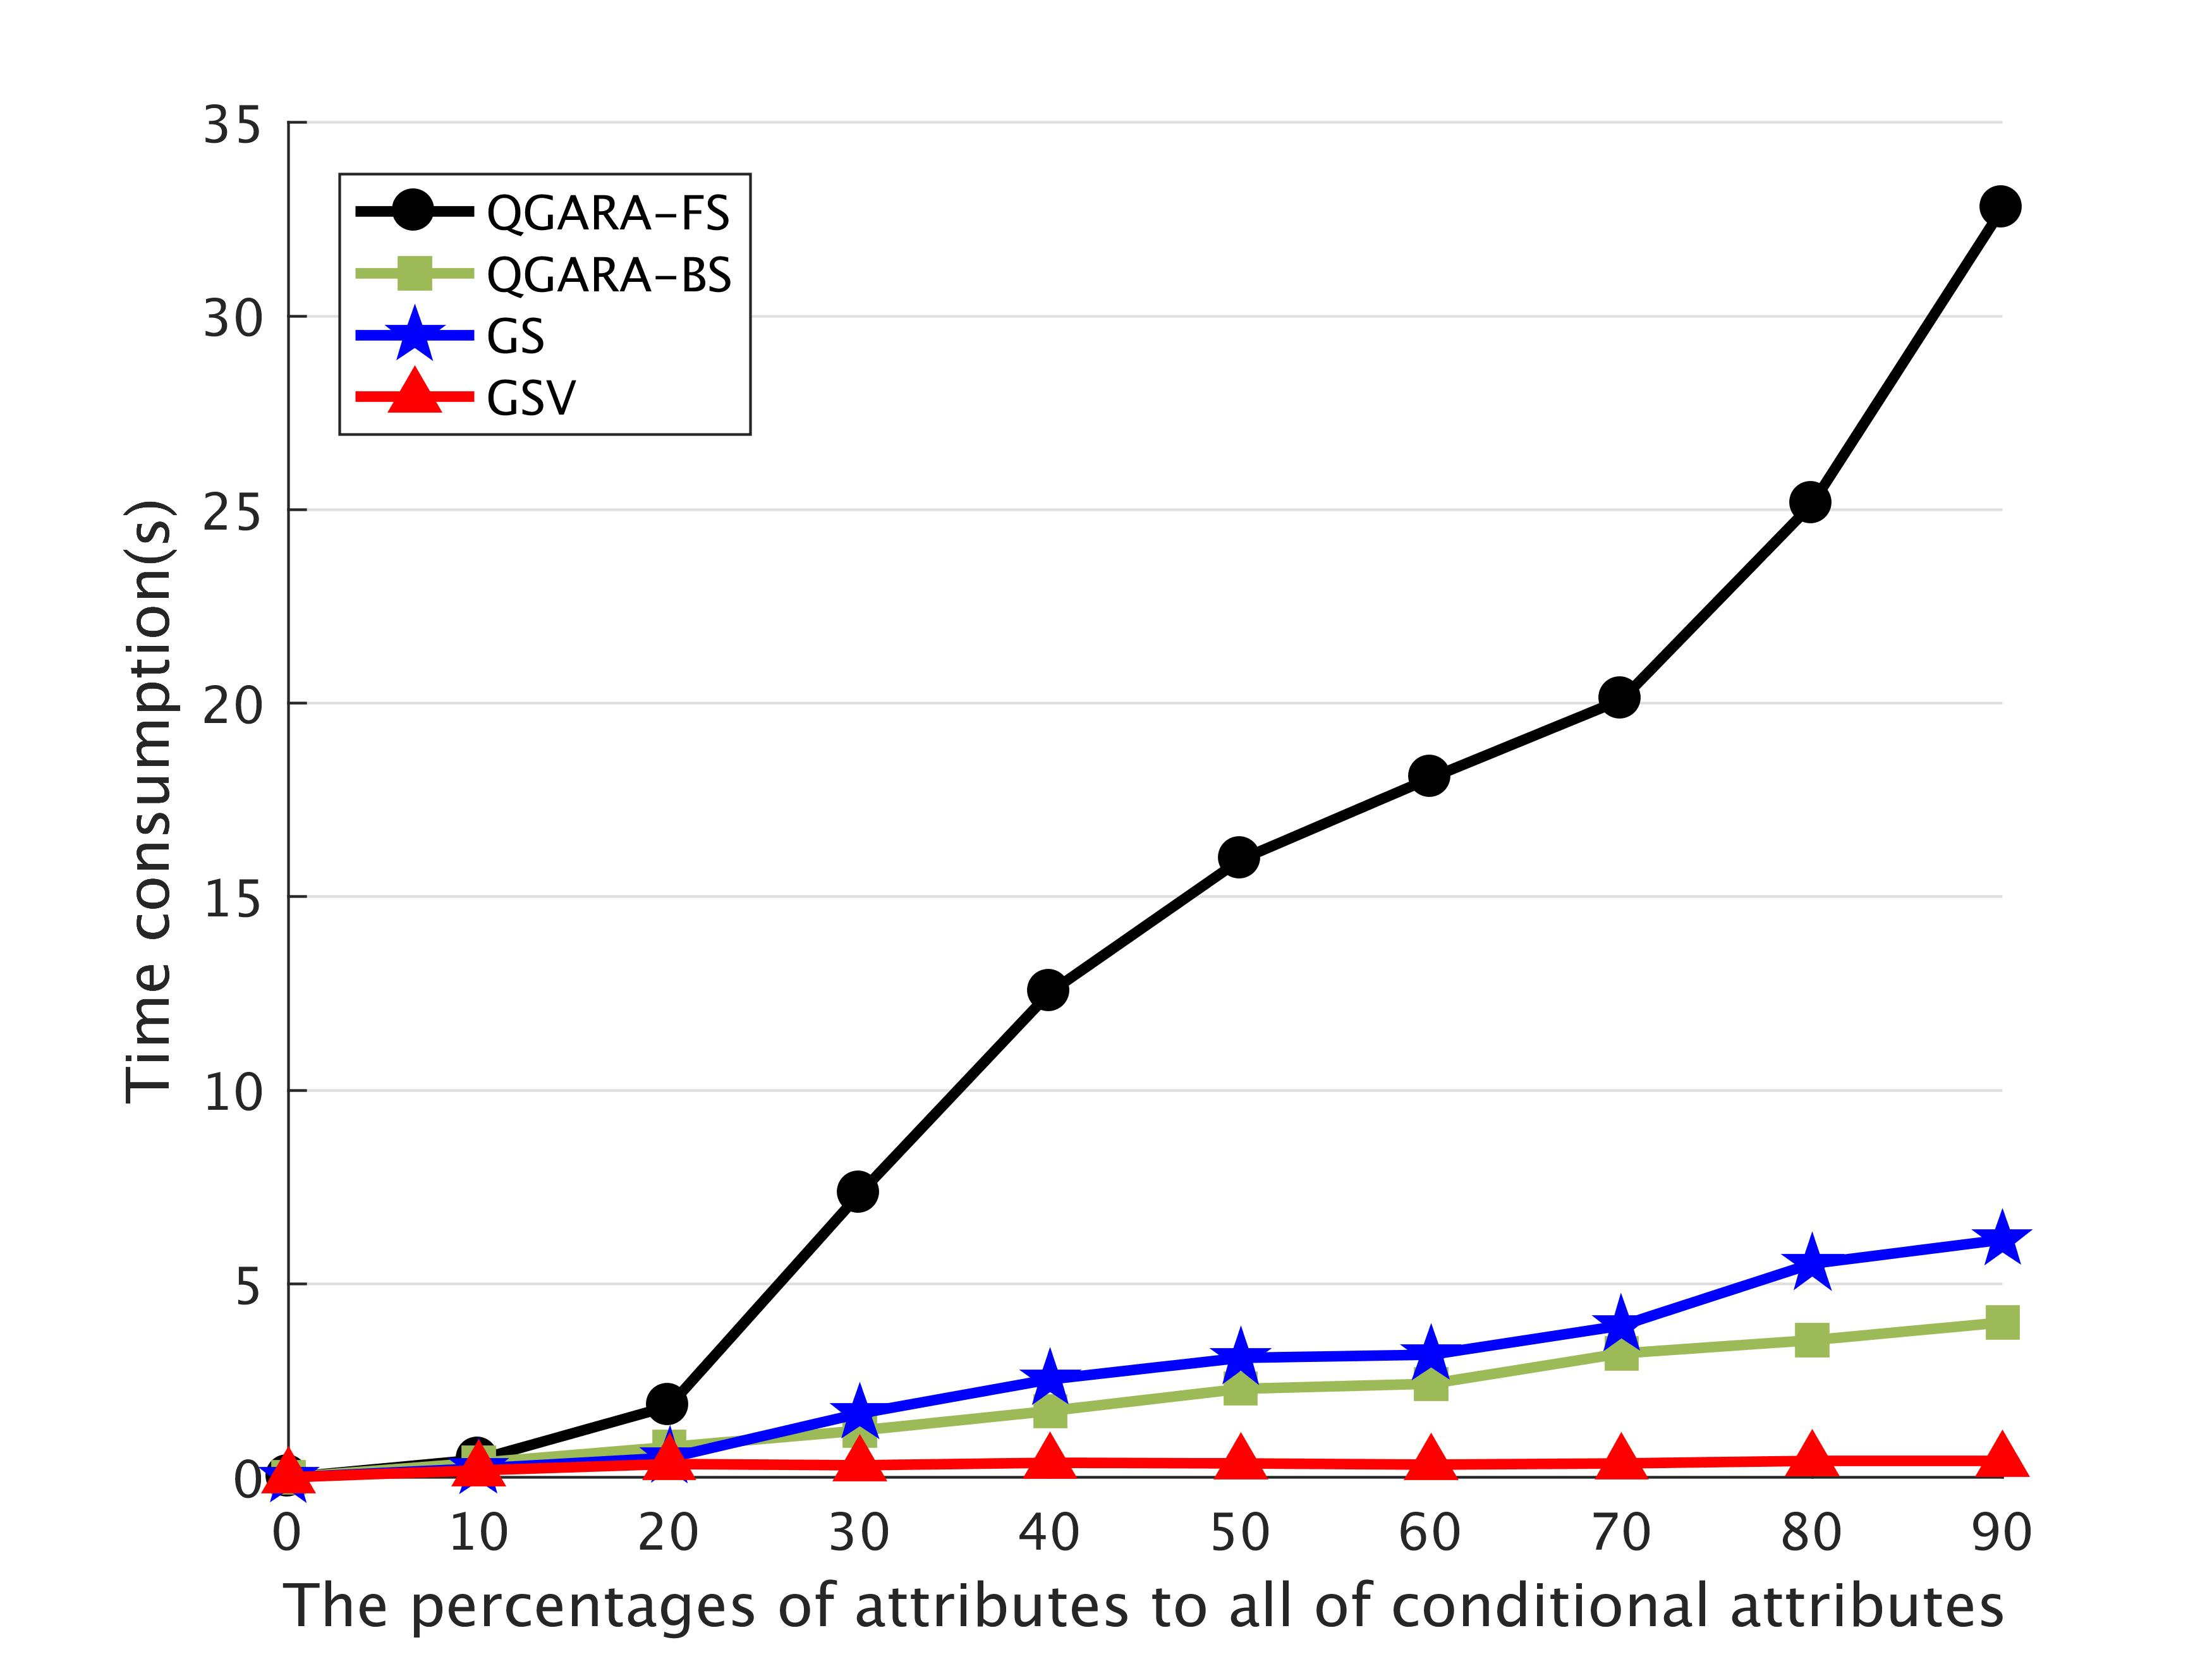
\includegraphics[width=5cm]{./Curve_attributes/4_splice_pos.jpg} 
			}
			\subfigure[Dermatology]{
				\label{Fig.sub2.7}
				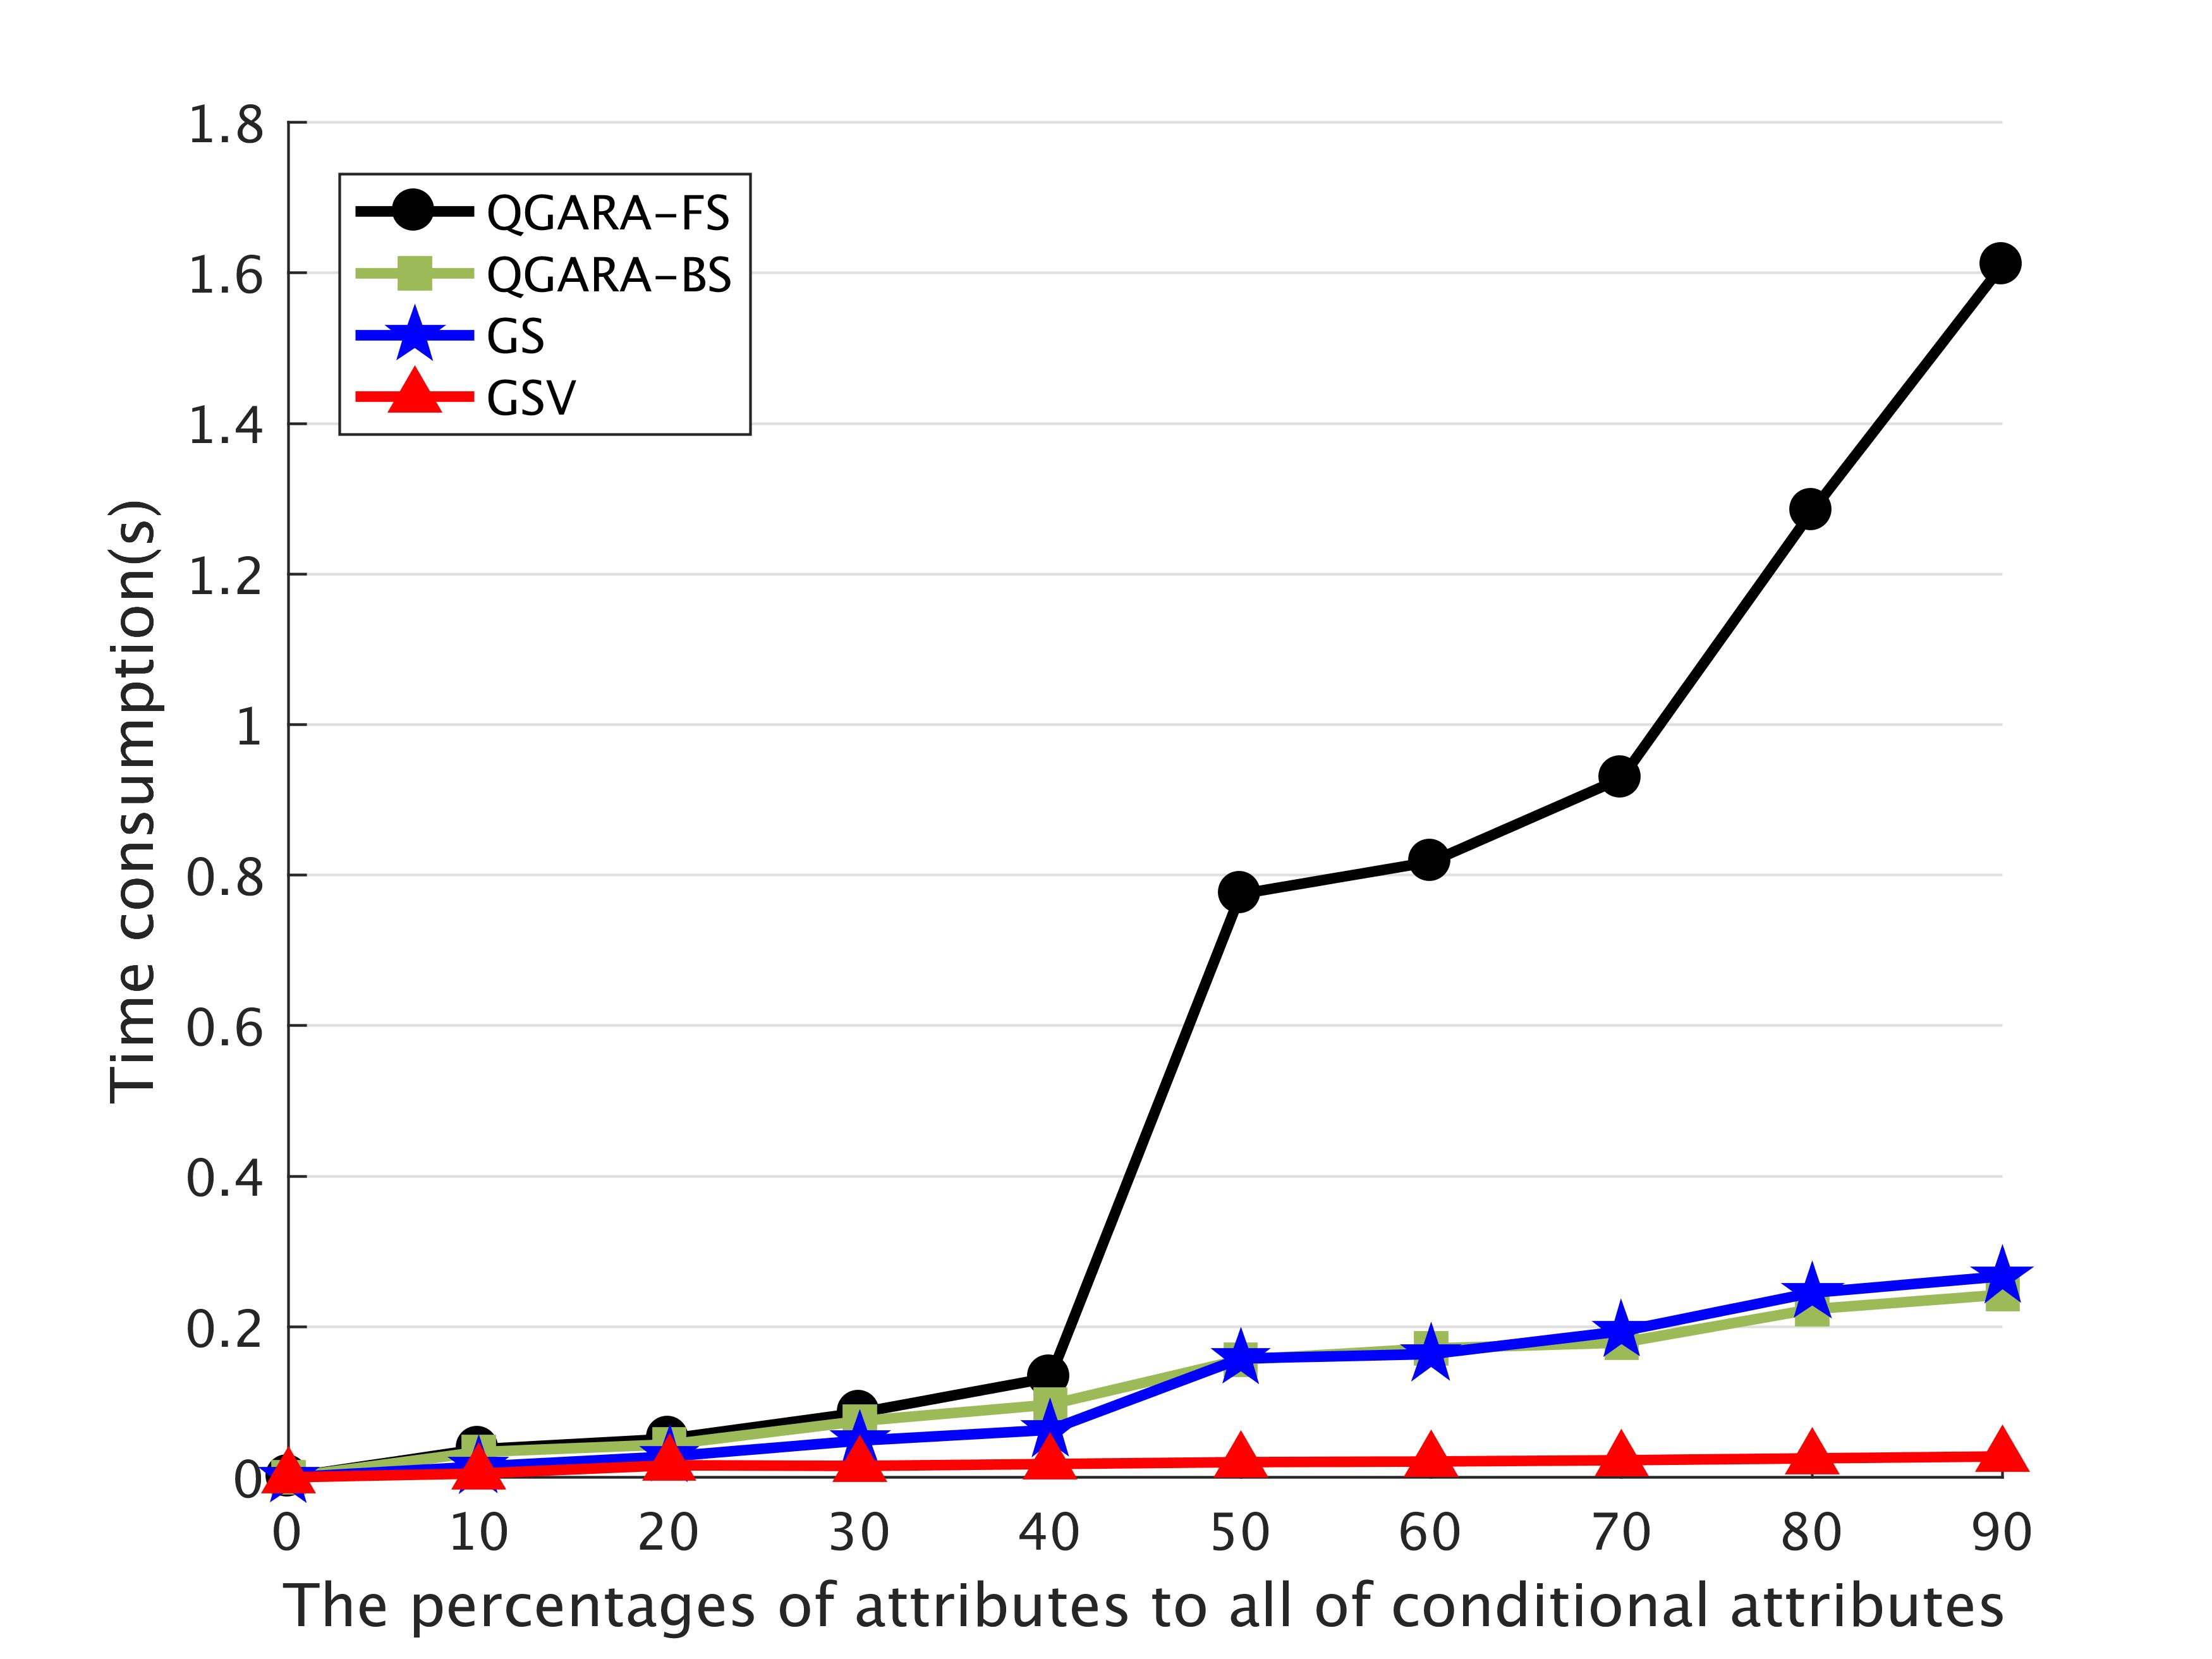
\includegraphics[width=5cm]{./Curve_attributes/5_dermatology_pos.jpg} 
			}
			\subfigure[Wdbc]{
				\label{Fig.sub2.8}
				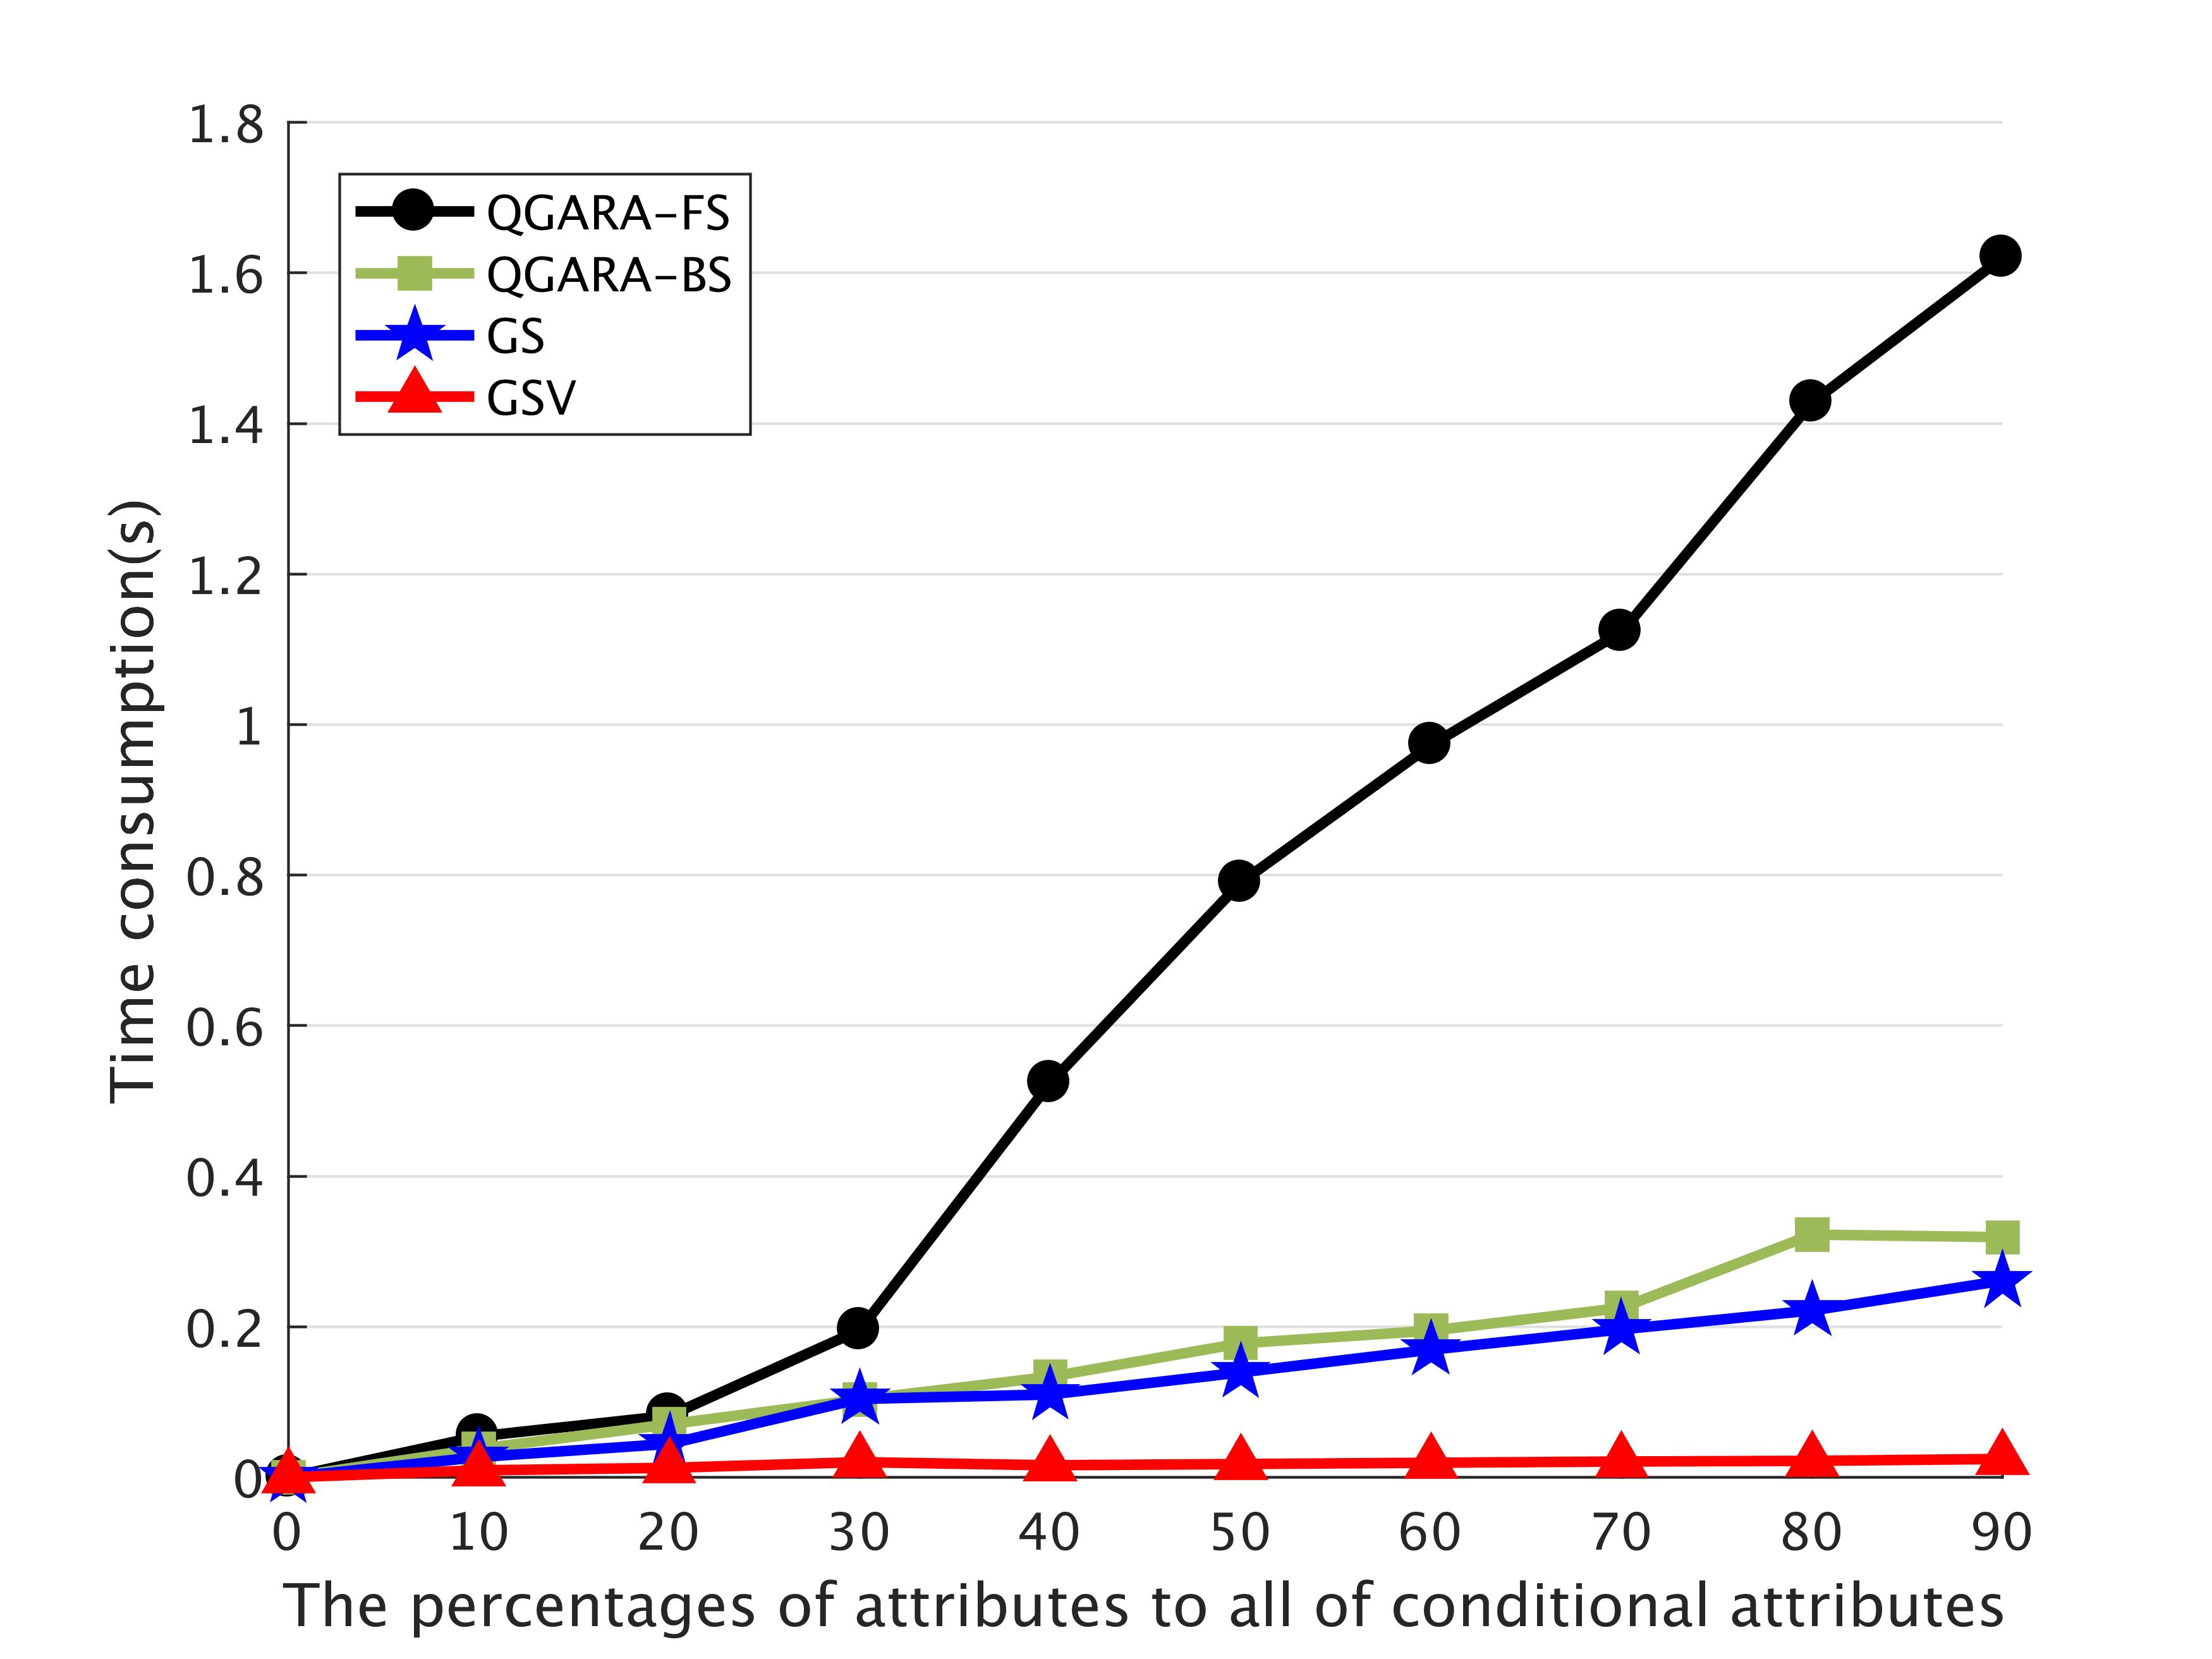
\includegraphics[width=5cm]{./Curve_attributes/6_wdbc_pos.jpg} 
			}
			%		\end{figure}
			%		\begin{figure}[htbp]
			\subfigure[CNAE9]{
				\label{Fig.sub2.9}
				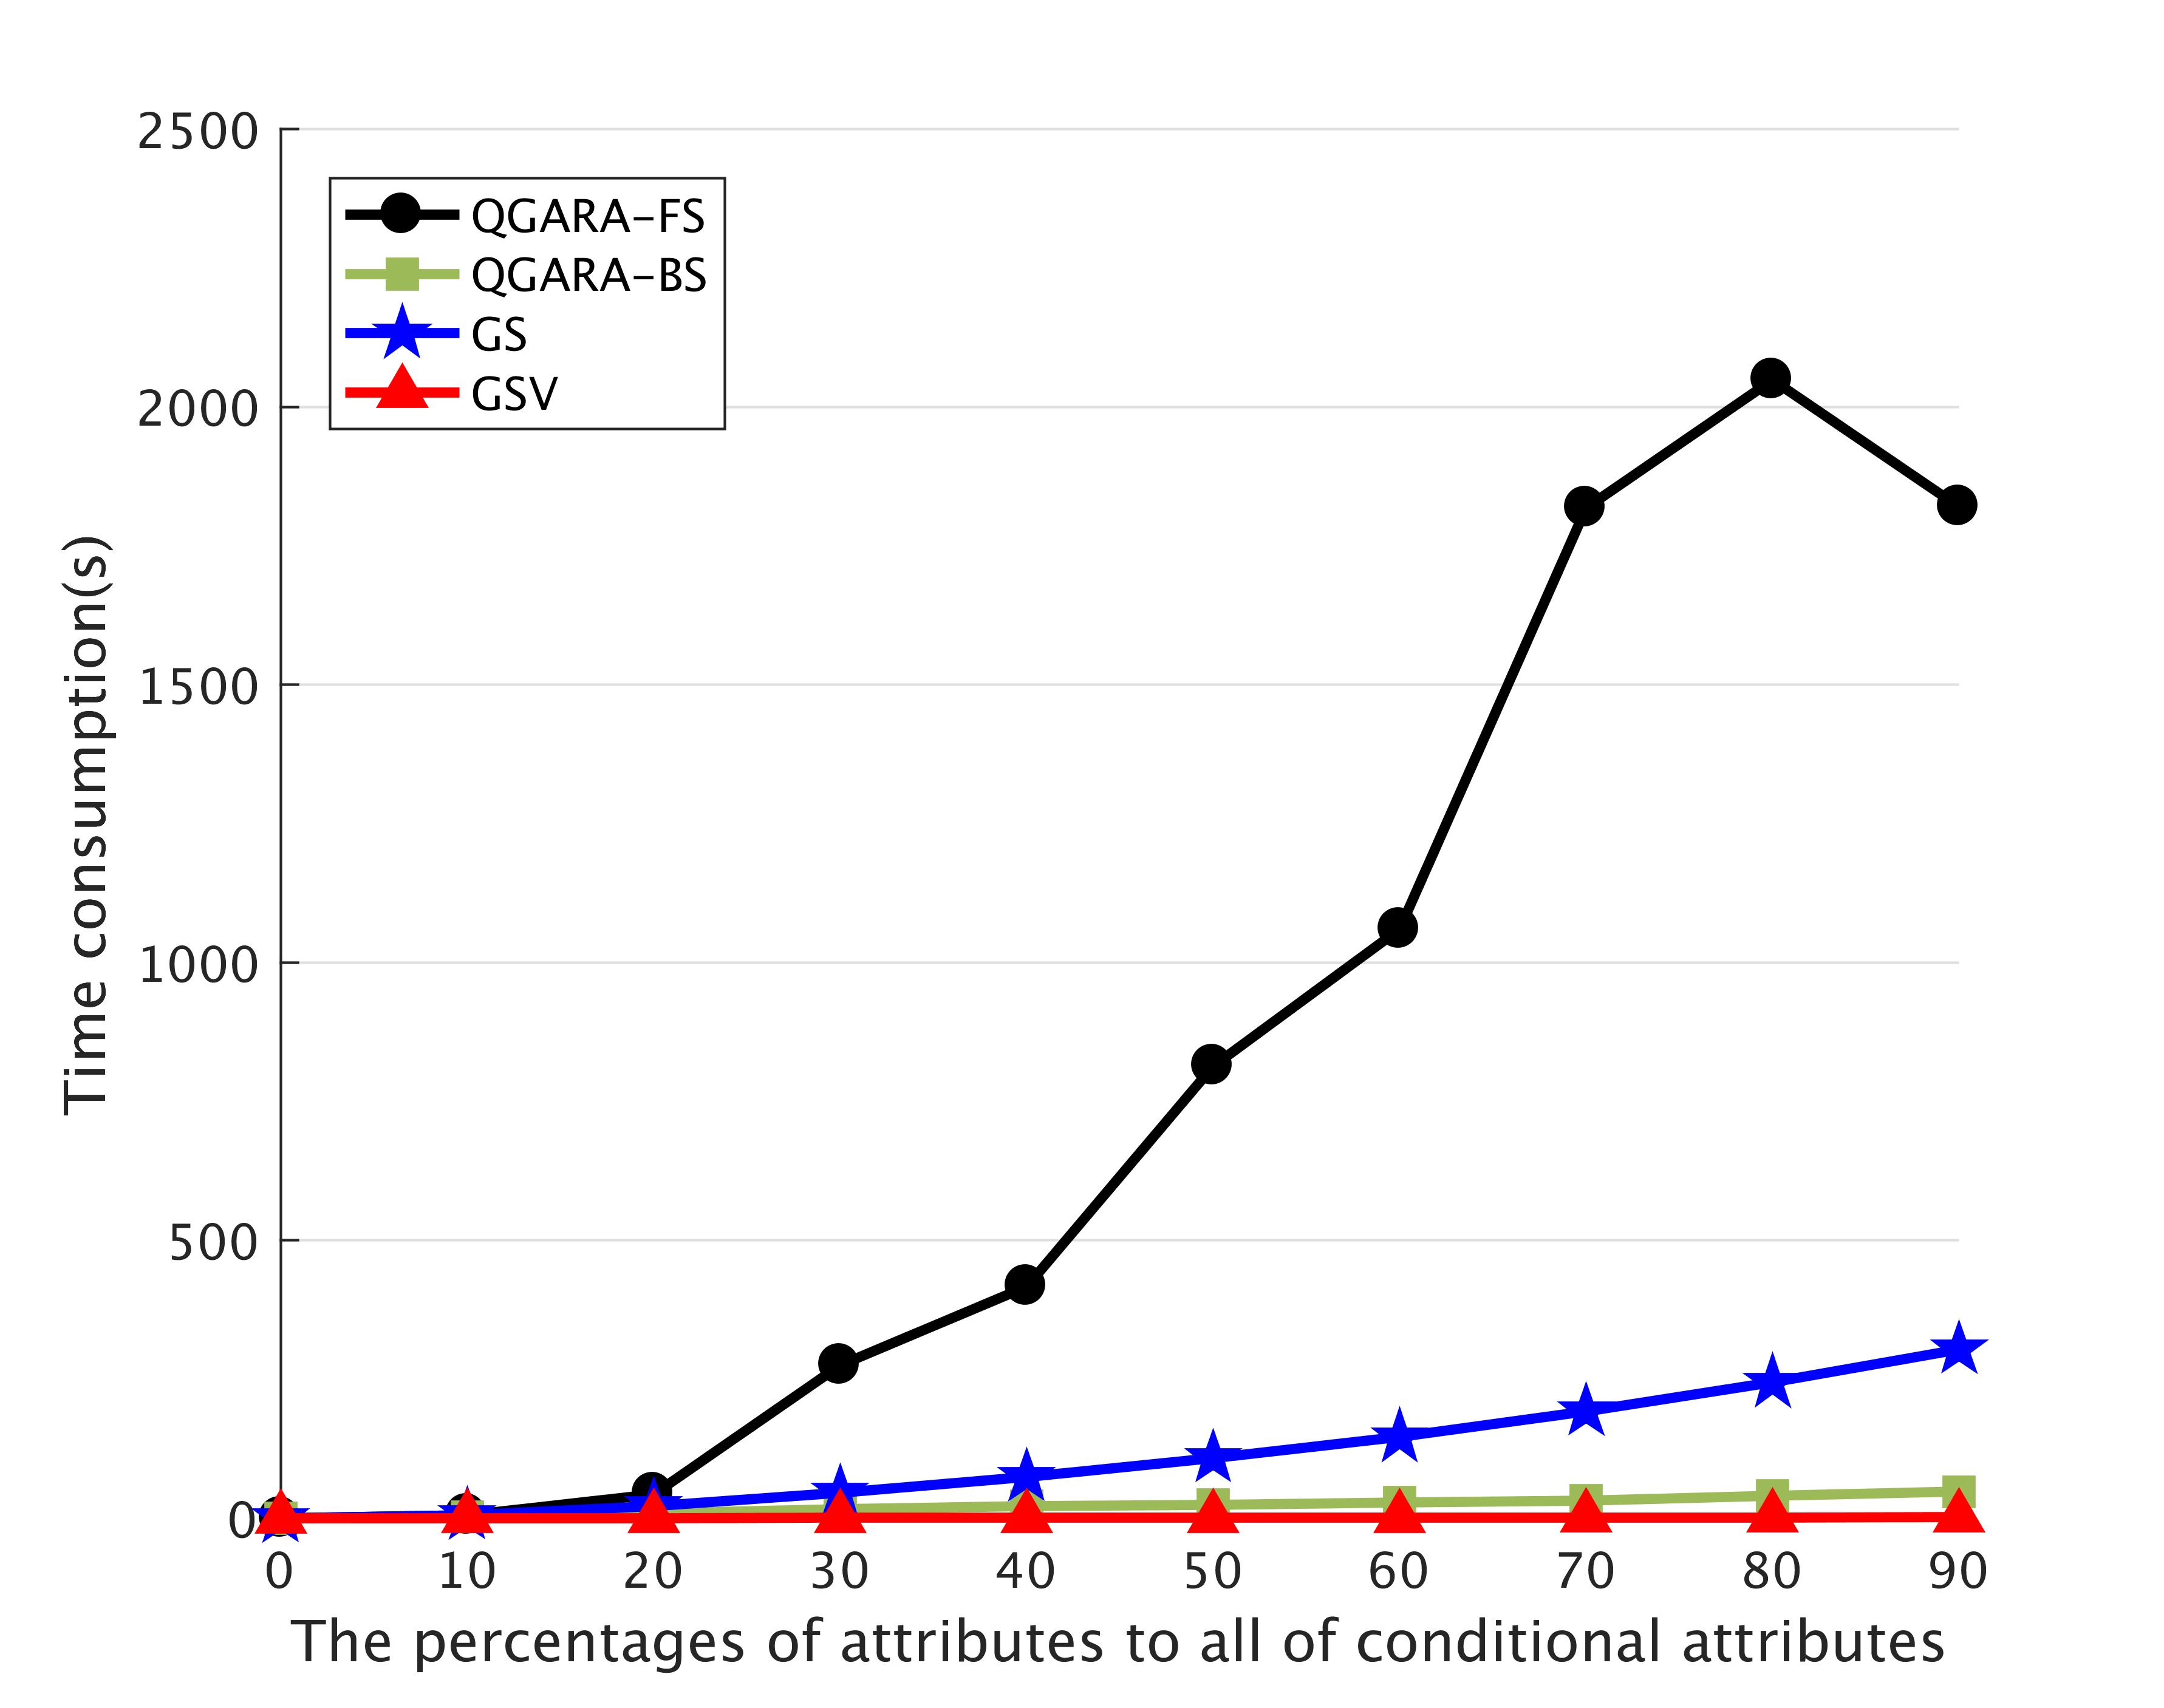
\includegraphics[width=5cm]{./Curve_attributes/9.jpg} 
			}
%			\subfigure[Semeion]{
%				\label{Fig.sub2.10}
%				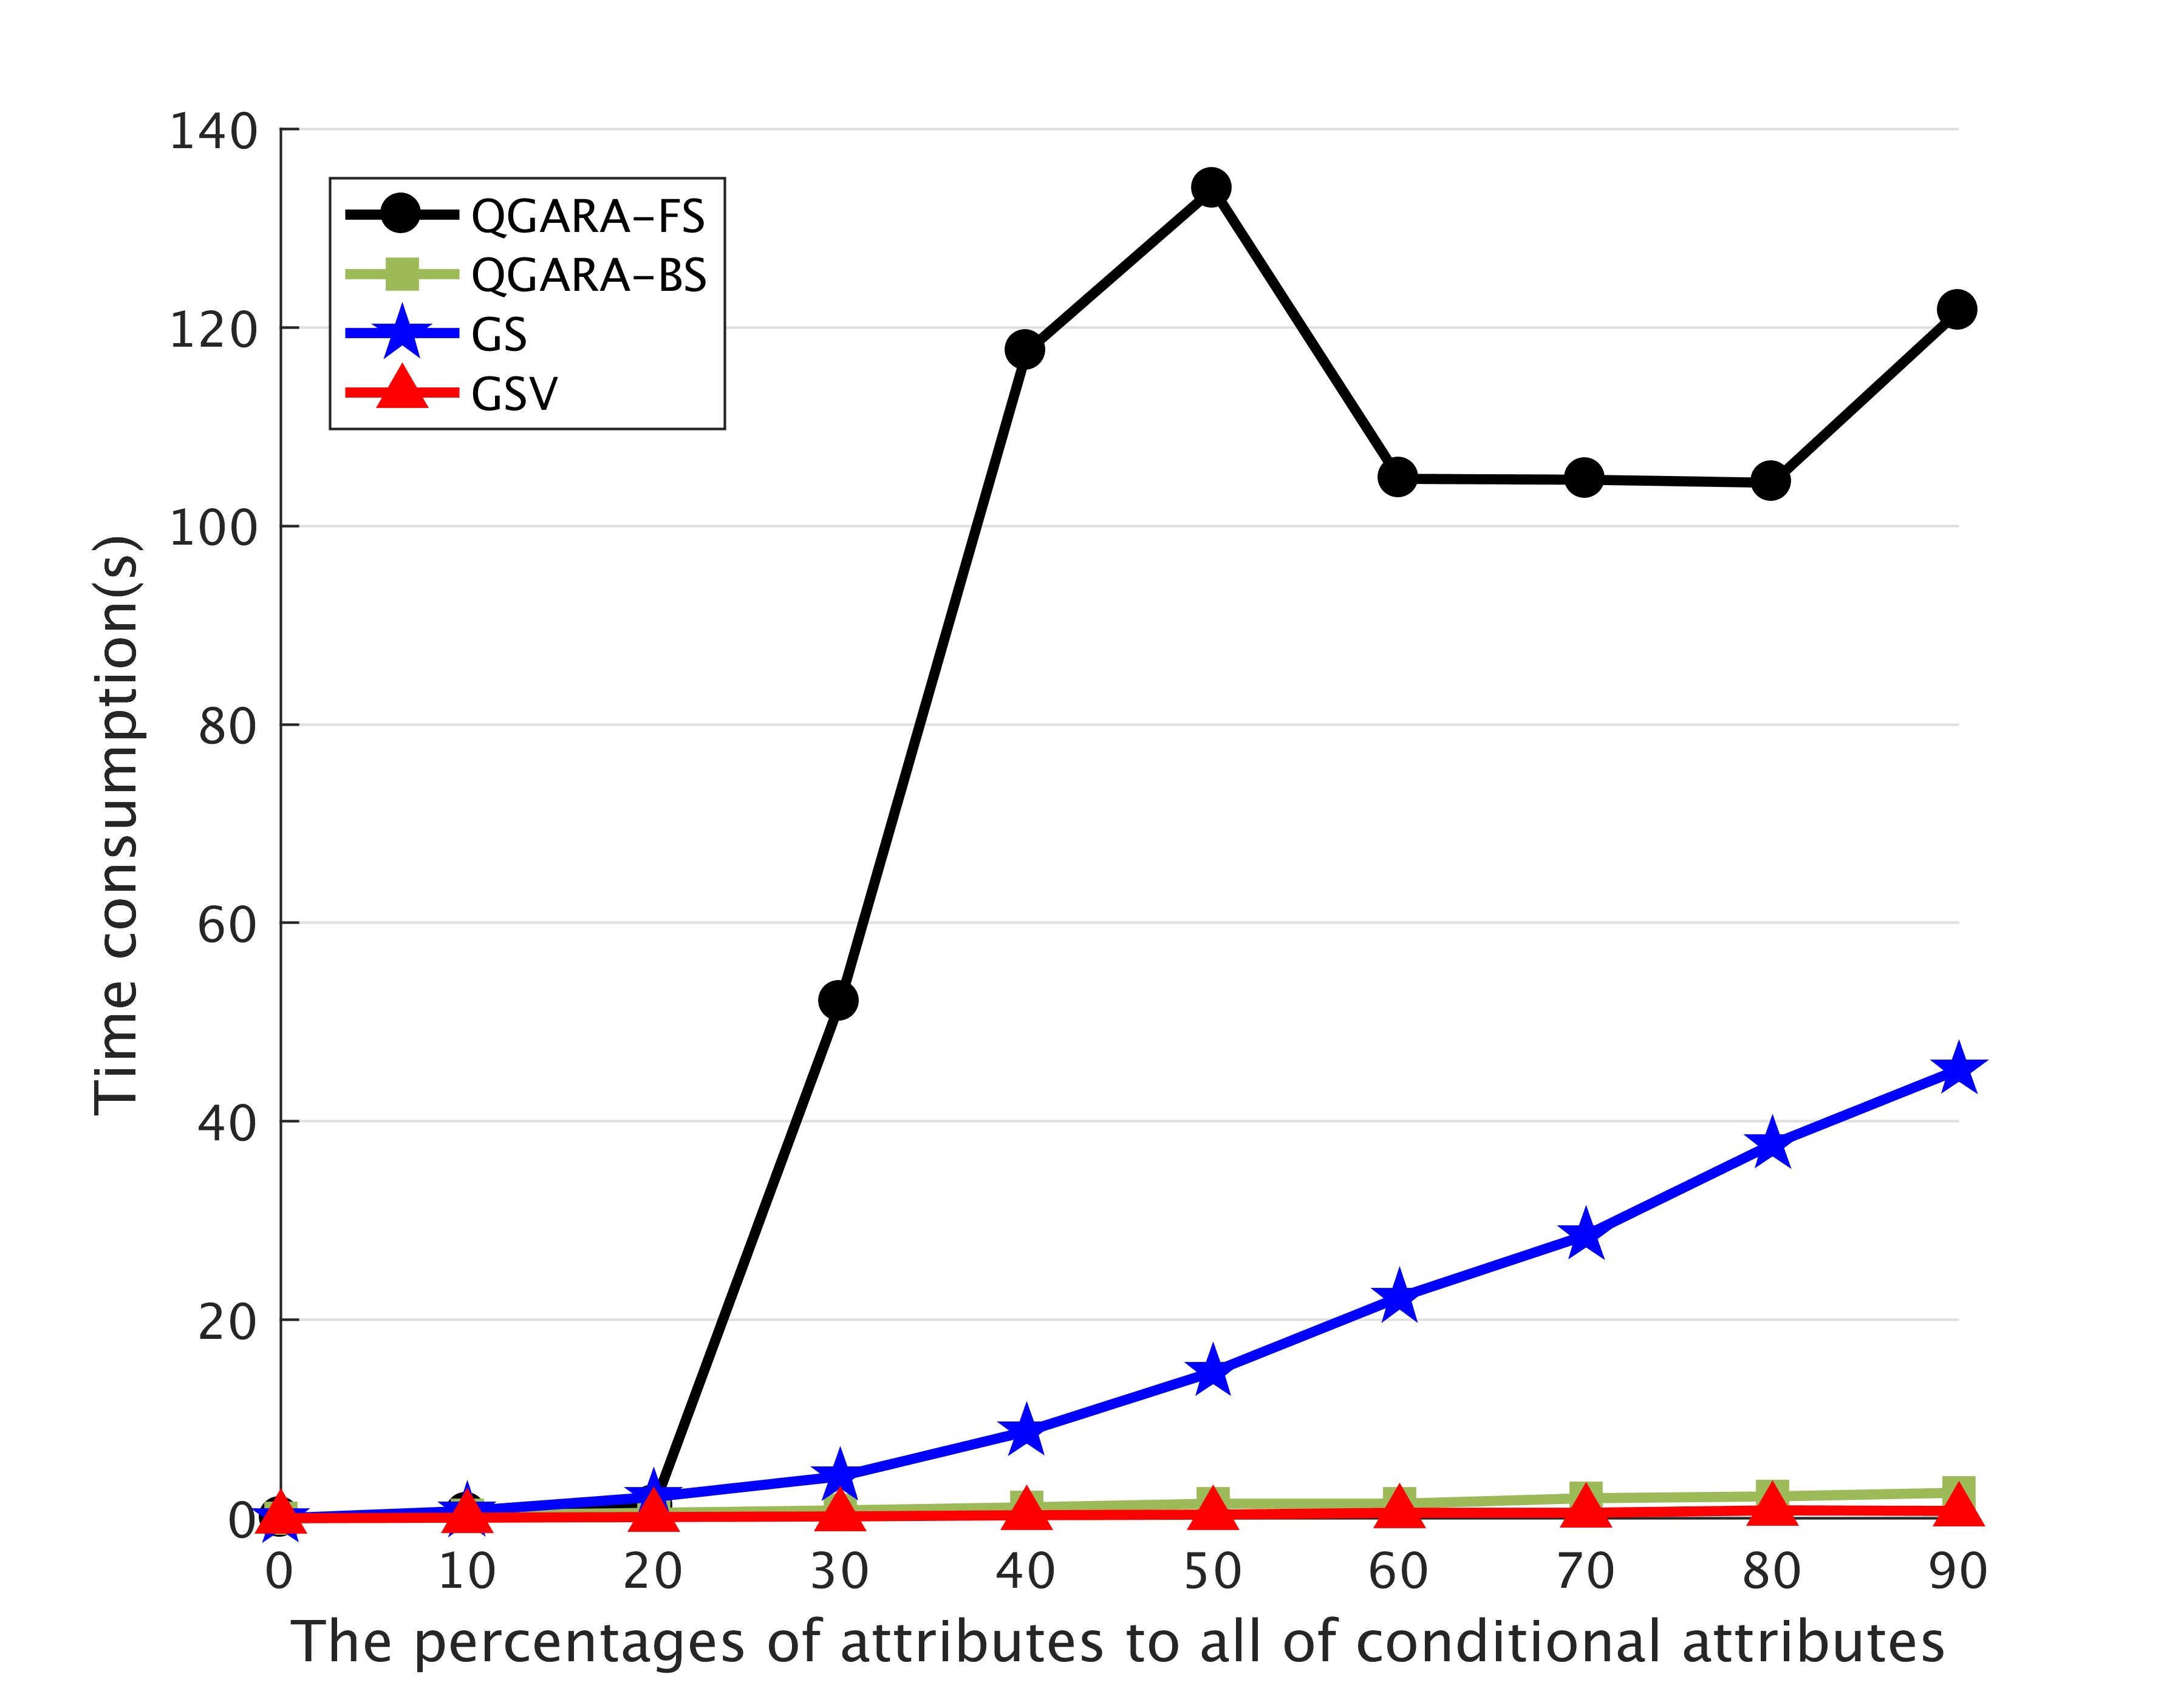
\includegraphics[width=5cm]{./Curve_attributes/10.jpg} 
%			}
			\subfigure[DNA]{
				\label{Fig.sub2.11}
				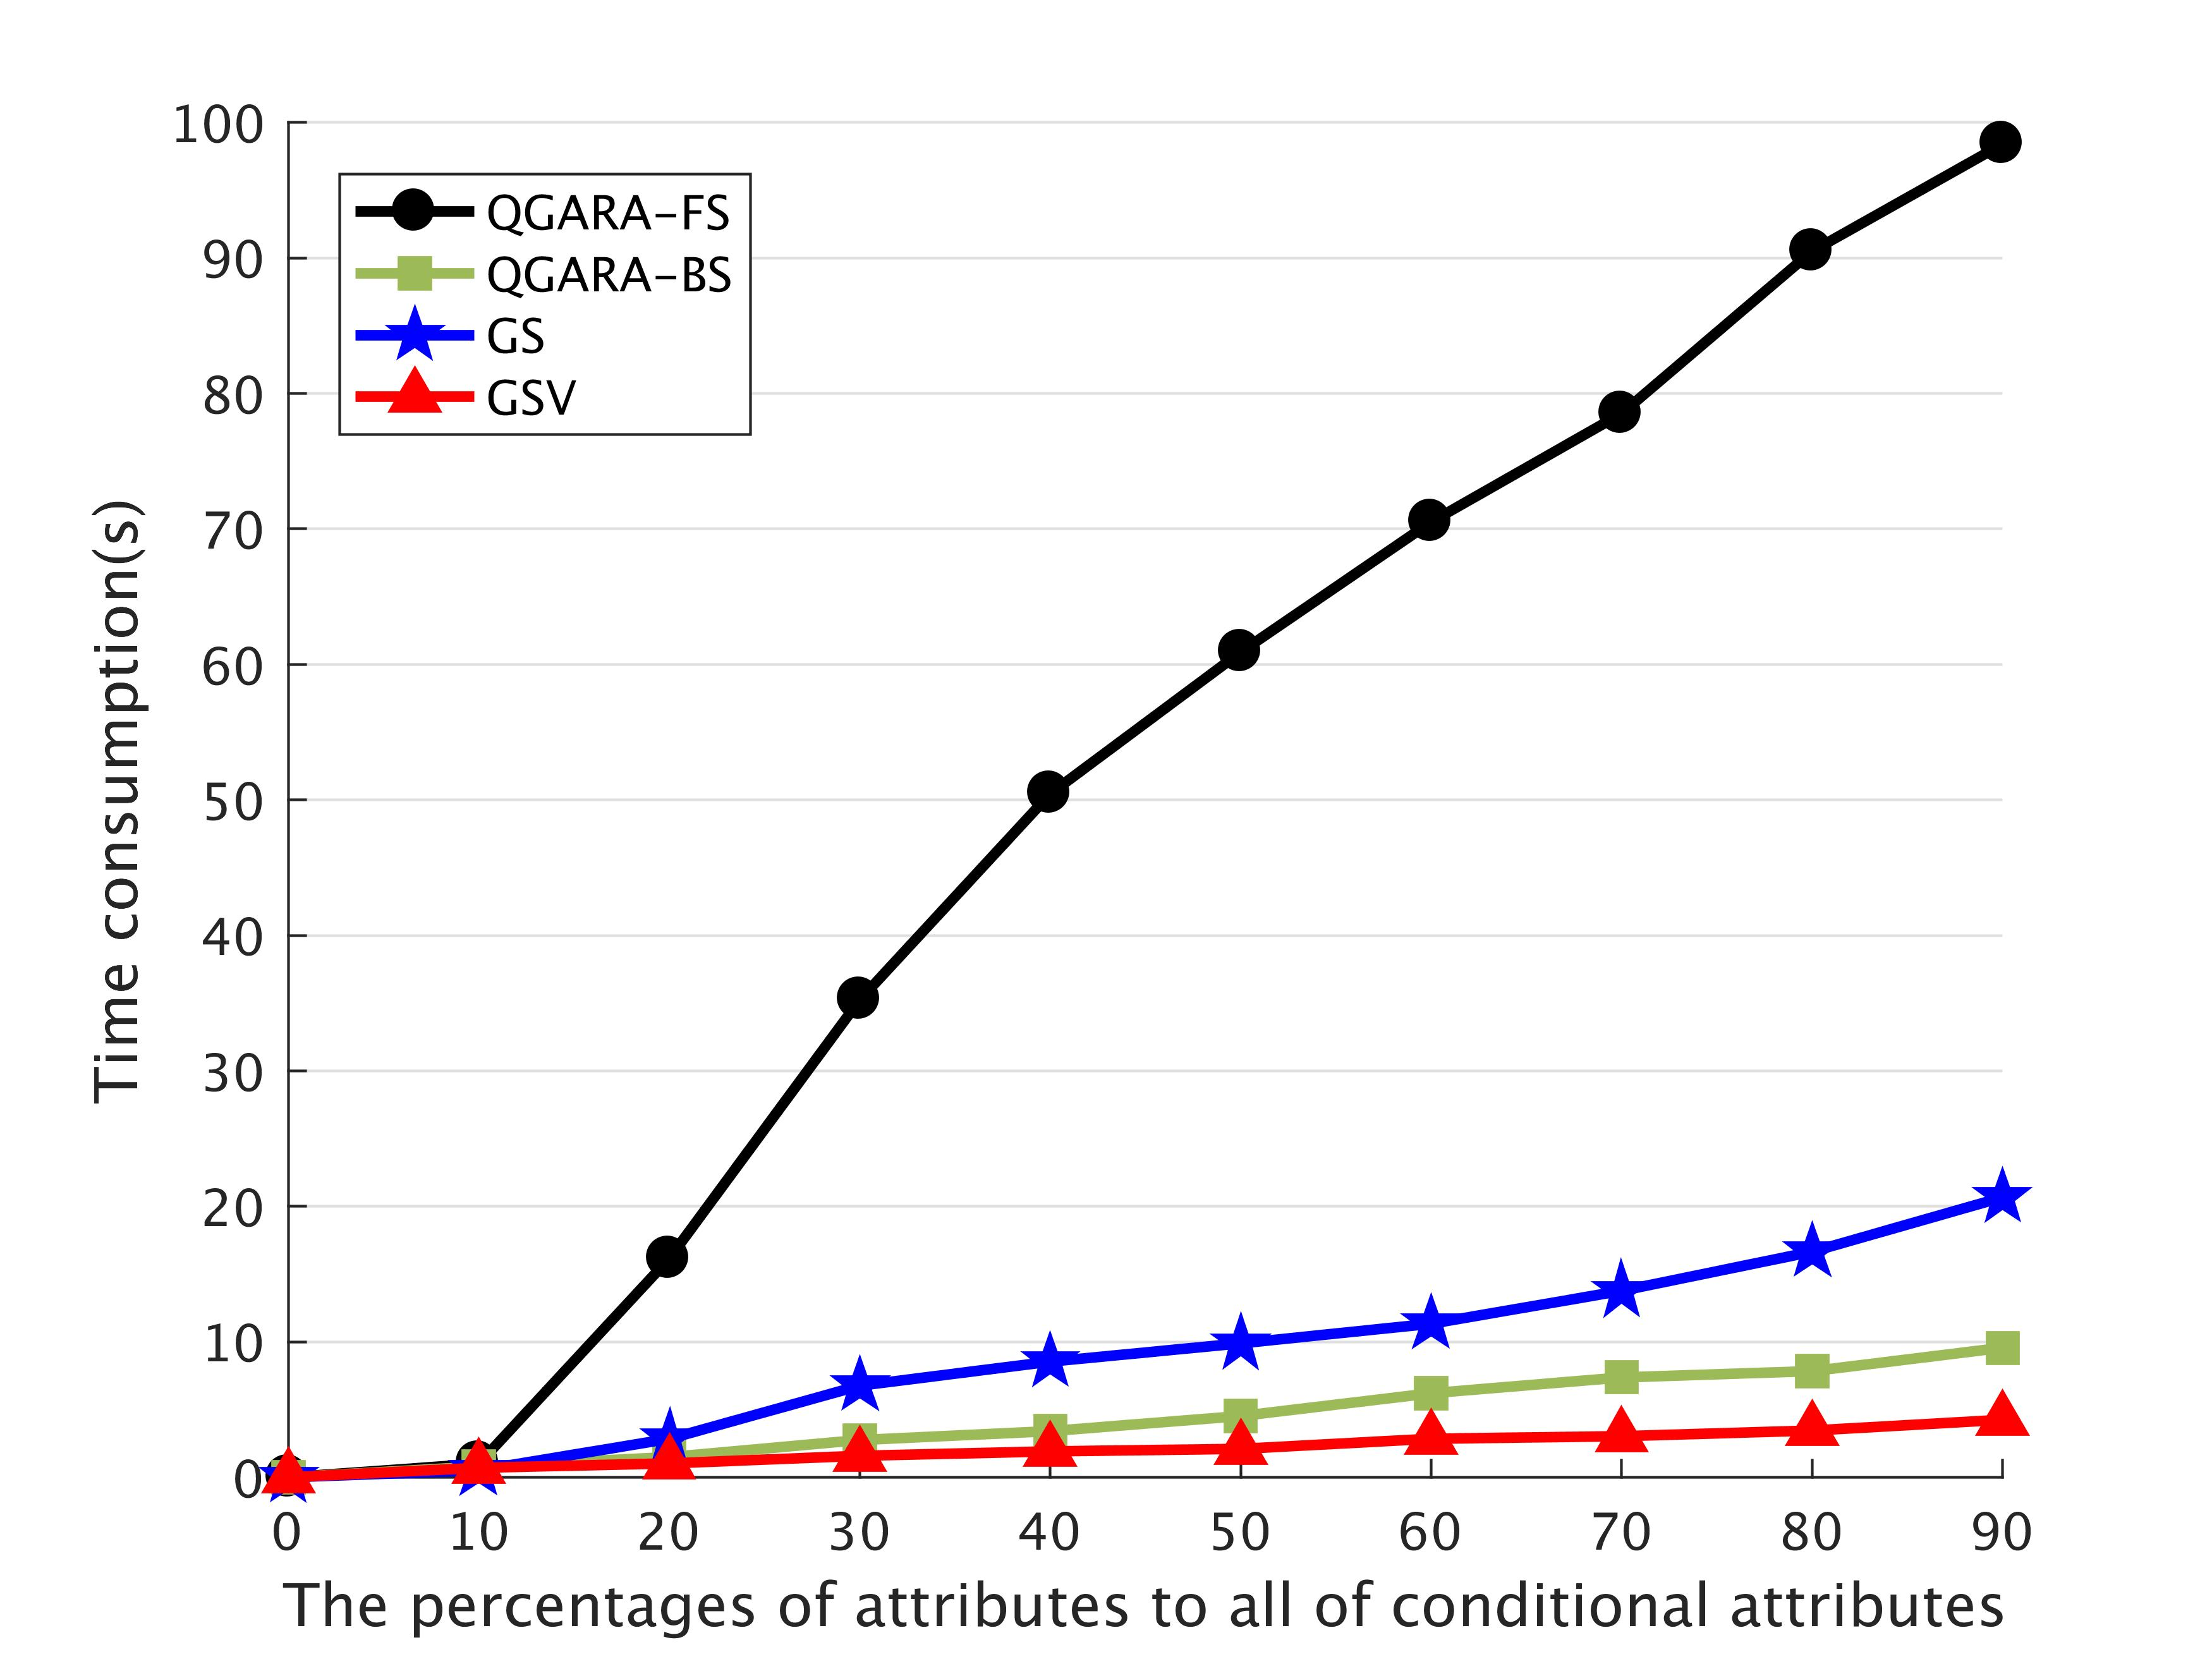
\includegraphics[width=5cm]{./Curve_attributes/9_dna_pos.jpg} 
			}
%			\subfigure[connect4]{
%				\label{Fig.sub2.12}
%				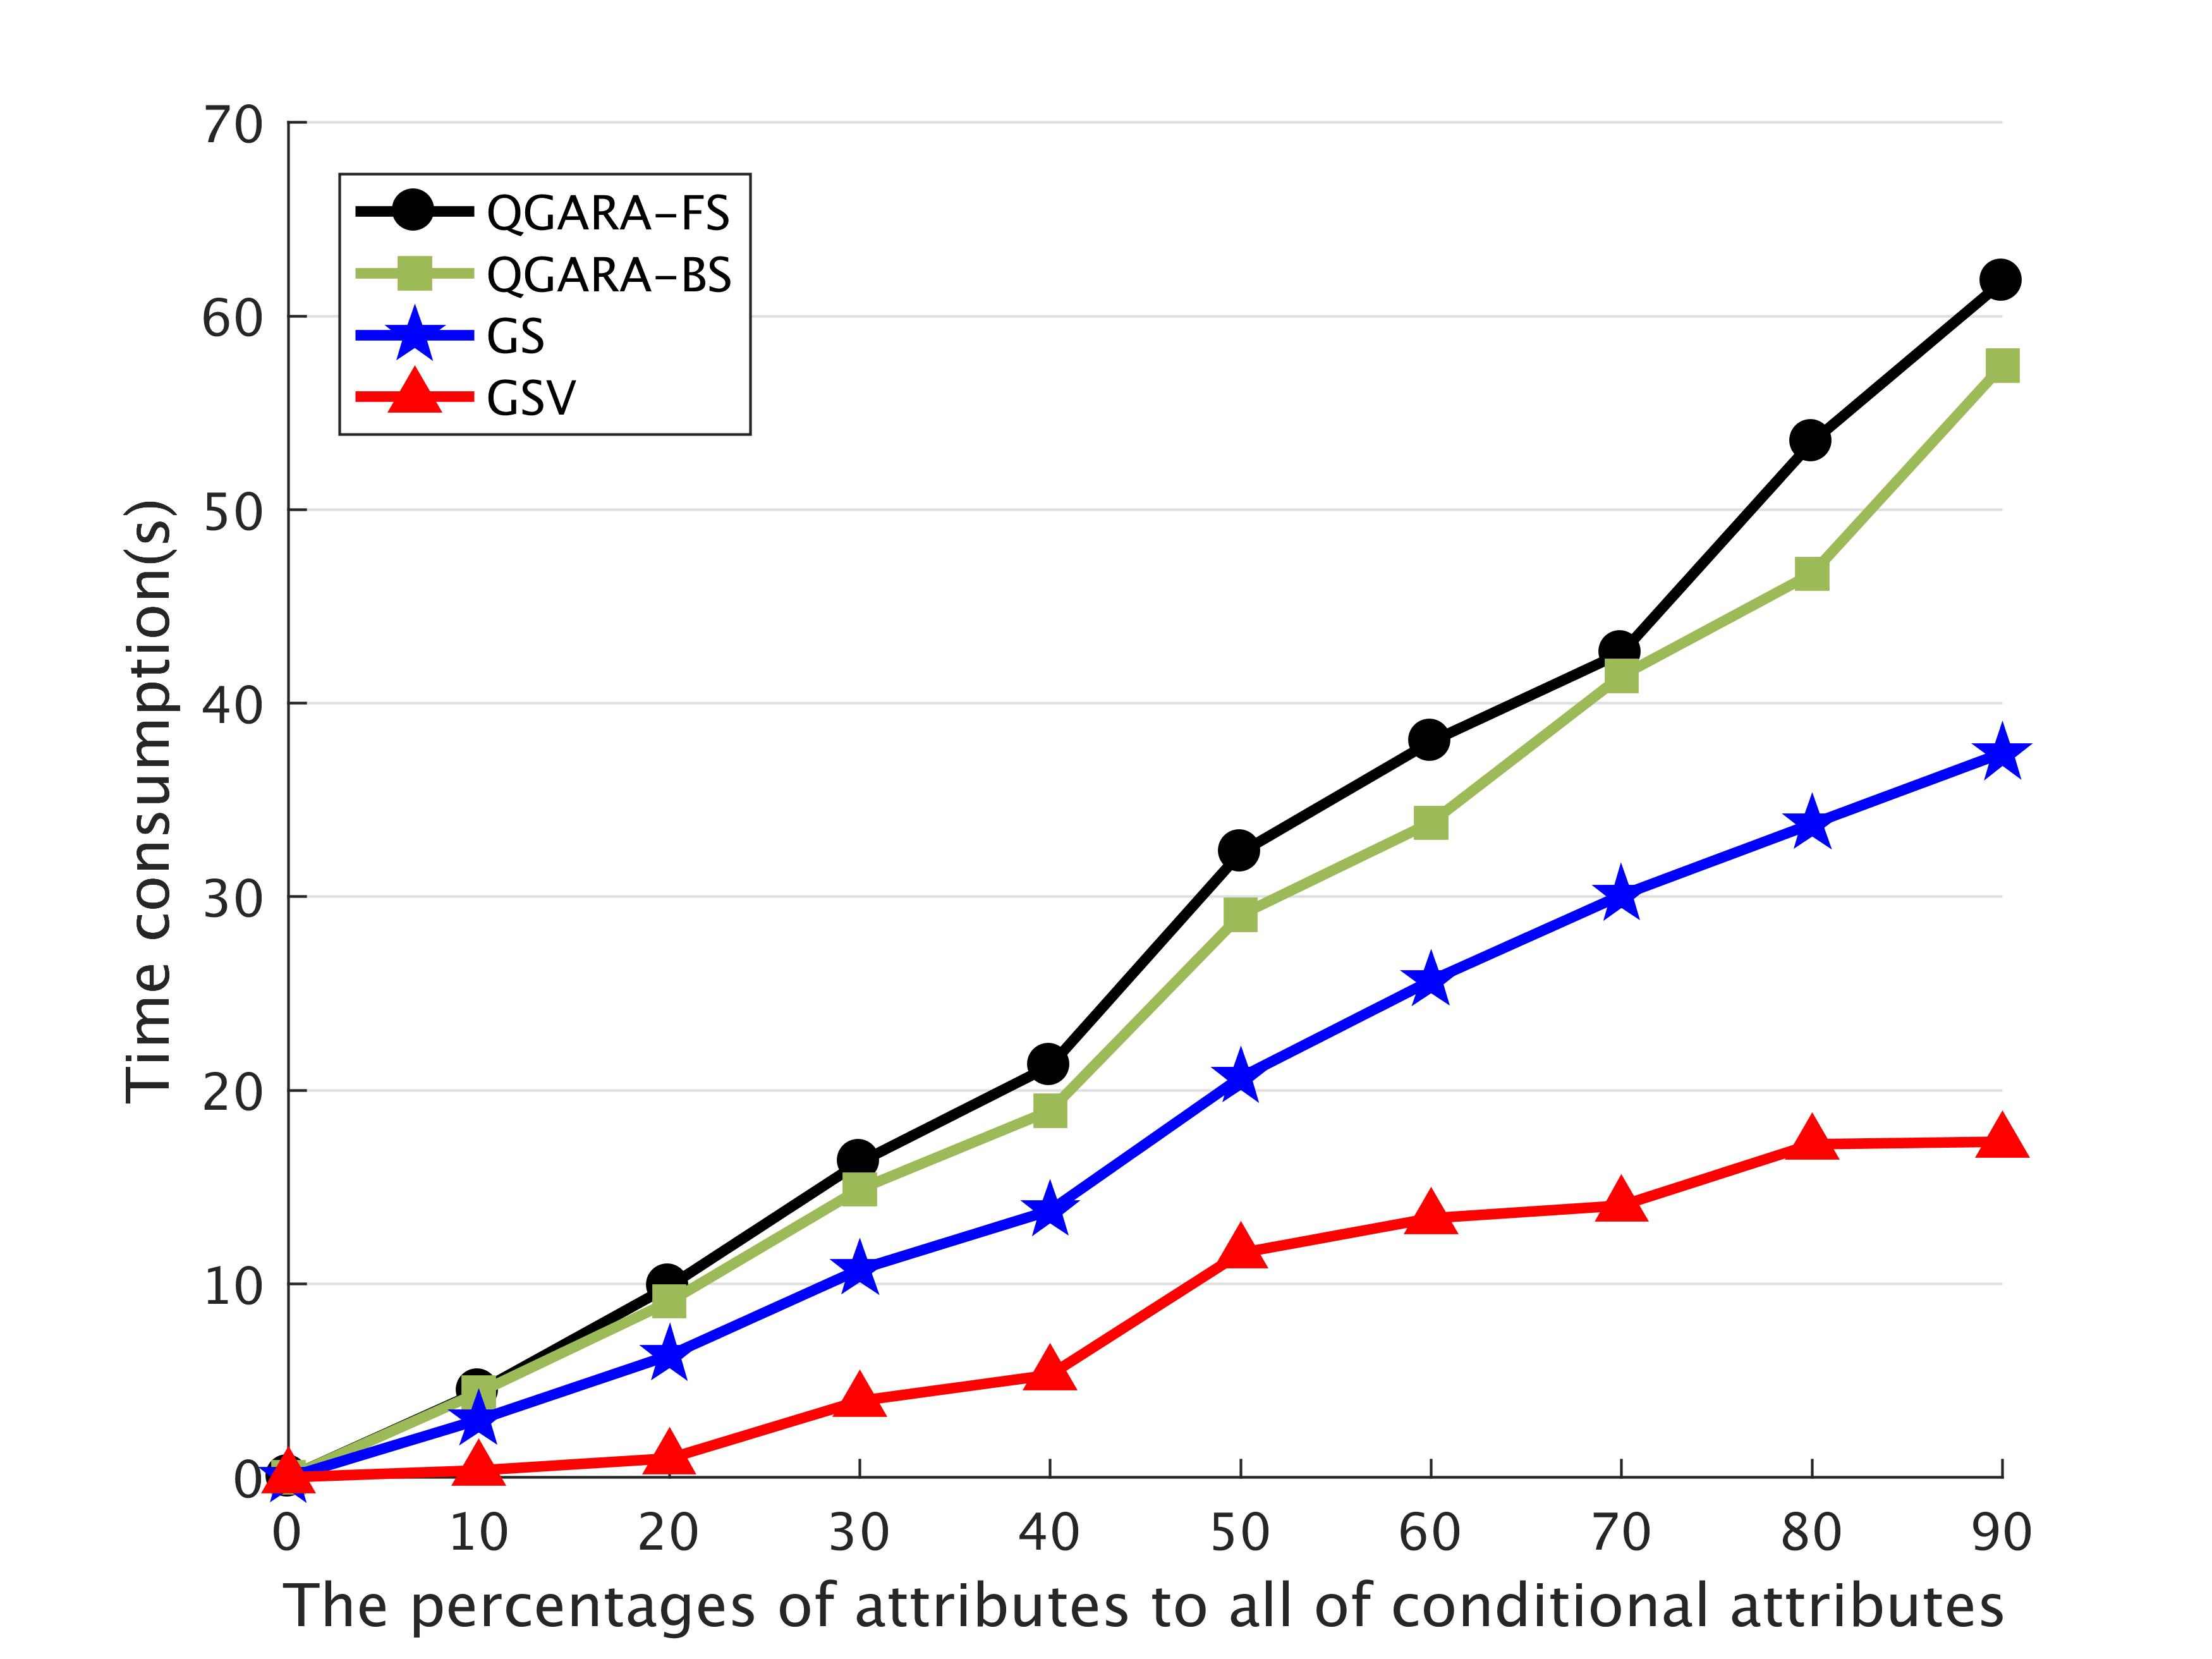
\includegraphics[width=5cm]{./Curve_attributes/10_connect4_pos.jpg} 
%			}
			\caption{The time of general reduction algorithms versus the size of attributes} 
			\label{TimeIncreaseAttributes}
		\end{figure}
		\par In Figure \ref{TimeIncreaseAttributes}, the x-coordinate pertains to the percentages of attributes to the conditional attributes of the data set, while the y-coordinate concerns the time consumption of algorithms. We took 8 data sets (Mushroom, Tic, Segmentation, Splice, Dermatology, Wdbc, CNAE9, and DNA) to verify the performance of the computational time of QGARA-FS, QGARA-BS, GS, and GSV for obtaining a relative discernibility realtion preservation reduct. The result of QGARA-FS, QGARA-BS, GS, and GSV was similar to the result induced from Figure \ref{TimeIncreaseObjects}.
	
	\subsection{Comparison of classification accuracy for general attribute reduction algorithms}
		\par As we know, there are many factors to the diversity of reducts obtained by reduction algorithms, such as reduction criterion, search strategy, and heuristic functions used, etc. That is to say, the different general reduction algorithms with the same reduction criterion may generate different reducts. To evaluate the effect of reduct obtained by different general reduction algorithms, we randomly selected 10 data sets as test objects from Table \ref{uci}. We utilized the original data and the reduced data, which is generated by five algorithms QGARA-FS, QGARA-BS, GS, GSV, and chi-square feature selection(CSFS for short), to train naive bayes classifier and decision tree classifier based on the 10-fold cross-validation method. For chi-square feature selection, naive bayes classifier, and decision tree classifier, we used its implementation in \cite{scikit-learn}. Regarding the parameter $K$ in CSFS, determining how many attributes are contained in reduced data, we assigned $K$ as the cardinality of the reduct generated by GS. It is worth noticing that CSFS is not related to attribute reduction in theory and the reason why we put it into comparisons is to do the evaluation of GS and GSV in feature selection perspective. For convenience of comparison, we take the output of CSFS as a PRPR when $K$ is assigned with the cardinality of the PRPR generated by GS; we take the output of CSFS as a DRPR when $K$ is assigned with the cardinality of the DRPR generated by GS. The classification accuracy to the raw data and the reduced data generated by different algorithms were shown in Tables \ref{cadtp} to \ref{canbd}, where the column "Raw" represents the classification accuracies of the classifier trained on raw data sets, the boldface highlights the highest accuracy among different algorithms, and the row "Average" represents average classification accuracy of reduction algorithms on 10 data sets, which can be interpreted as an estimated value of classification accuracy obtained by the output of related reduction algorithm over unknown data sets.  
		\begin{table}[htb]
			\centering
			\caption{The classification accuracy of decision tree with PRPR found by five algorithms}
			\begin{tabular}{ccccccc}
				\hline%\toprule
				ID    & Raw   & QGARA-FS & QGARA-BS & GS    & GSV   & CSFS \\
				\hline%\midrule
				2     & 0.551 & 0.603 & 0.608 & \textbf{0.614} & 0.574 & 0.599 \\
				3     & 0.896 & 0.892 & 0.898 & 0.897 & 0.896 & \textbf{0.901} \\
				4     & 0.943 & 0.938 & 0.937 & 0.937 & \textbf{0.939} & 0.825 \\
				5     & 0.685 & 0.687 & 0.689 & 0.682 & 0.689 & \textbf{0.695} \\
				6     & 0.900 & 0.656 & 0.449 & 0.760 & 0.804 & \textbf{0.872} \\
				7     & 0.936 & 0.604 & 0.735 & 0.789 & \textbf{0.867} & 0.685 \\
				8     & 0.926 & \textbf{0.940} & 0.905 & 0.916 & 0.933 & 0.935 \\
				9     & 0.856 & 0.873 & 0.859 & 0.870 & \textbf{0.874} & 0.867 \\
				11    & 0.901 & 0.857 & 0.494 & 0.871 & 0.580 & \textbf{0.932} \\
				12    & 0.476 & 0.478 & 0.462 & \textbf{0.481} & 0.475 & 0.471 \\
				\hline%\midrule
				Average & 0.807 & 0.753 & 0.704 & \textbf{0.782} & 0.763 & 0.778 \\
				\hline%\bottomrule
			\end{tabular}%
			\label{cadtp}%
		\end{table}%
		Obviously, for most of reduced data sets, reduced data can retain similar classification accuracy as the entire data set. 
		\begin{table}[htb]
			\centering
			\caption{The classification accuracy of decision tree with DRPR found by five algorithms}
			\begin{tabular}{ccccccc}
				\hline%\toprule
				ID    & Raw   & QGARA-FS & QGARA-BS & GS    & GSV   & CSFS \\
				\hline%\midrule
				2     & 0.551 & 0.554 & 0.551 & 0.558 & 0.551 & \textbf{0.584} \\
				3     & 0.896 & 0.896 & 0.898 & 0.897 & 0.894 & \textbf{0.900} \\
				4     & 0.943 & 0.938 & 0.940 & 0.938 & \textbf{0.942} & 0.819 \\
				5     & 0.685 & 0.682 & 0.685 & 0.685 & \textbf{0.691} & 0.684 \\
				6     & 0.900 & 0.651 & 0.455 & 0.762 & 0.809 & \textbf{0.873} \\
				7     & 0.936 & 0.590 & 0.746 & 0.787 & \textbf{0.878} & 0.685 \\
				8     & 0.926 & \textbf{0.938} & 0.902 & 0.907 & 0.931 & 0.933 \\
				9     & 0.856 & \textbf{0.872} & 0.853 & 0.870 & 0.871 & 0.862 \\
				11    & 0.901 & 0.861 & 0.502 & 0.868 & 0.580 & \textbf{0.933} \\
				12    & 0.476 & \textbf{0.477} & 0.466 & \textbf{0.477} & \textbf{0.477} & 0.472 \\
				\hline%\midrule
				Average & 0.807 & 0.746 & 0.700 & \textbf{0.775} & 0.762 & \textbf{0.775} \\
				\hline%\bottomrule
			\end{tabular}%
			\label{cadtd}%
		\end{table}%
		\par For Table \ref{cadtp}, the order of algorithms in the number of achieving the most classification accuracy is CSFS(4) $> $ GSV(3) $> $ GS(2)Q $> $ GARA-FS(1) $> $ QGARA-BS(0). The order of algorithms in the average of classification accuracy on 10 data sets is GS(0.782) $> $ CSFS(0.778) $> $ GSV(0.763) $> $ QGARA-FS(0.753) $> $ QGARA-BS(0.704). GS achieves the best average classification accuracy on 10 data sets. That is to say, the steadiness of algorithms QGARA-FS, QGARA-BS, CSFS, and GSV in classification accuracy is not as good as GS. Furthermore, the PRPR obtained by GS and GSV performs better than that obtained by QGARA-FS and QGARA-BS in the average classification accuracy of decision tree classifier. 
		When it comes to the reduced data generated in the criterion of relative discernibility relation preservation reduction, GSV and CSFS obtain the highest classification accuracy 4 times; QGARA-FS obtains the highest classification accuracy 3 times; GS obtains the highest classification accuracy 1 time; QGARA-BS obtains the highest classification accuracy 0 times. GSV and CSFS perform the best in times of achieving the best classification accuracy. Observing the average classification accuracy on ten data sets, GS is also the best of five, \emph{i.e.}, GS(0.775) $\geq$ CSFS(0.775) $> $ GSV(0.762) $> $ QGARA-FS(0.746) $> $ QGARA-BS(0.700). As a result, the DRPR obtained by GS and GSV performs better than that obtained by QGARA-FS and QGARA-BS in the average classification accuracy of decision tree classifier. 
		\begin{table}[htb]
			\centering
			\caption{The classification accuracy of naive bayes with PRPR found by five algorithms}
			\begin{tabular}{ccccccc}
				\hline%\toprule
				ID    & Raw   & QGARA-FS & QGARA-BS & GS    & GSV   & CSFS \\
				\hline%\midrule
				2     & 0.649 & 0.557 & 0.650 & 0.565 & 0.582 & \textbf{0.668} \\
				3     & 0.777 & 0.885 & 0.895 & \textbf{0.896} & \textbf{0.896} & 0.805 \\
				4     & 0.603 & 0.575 & 0.570 & 0.575 & \textbf{0.605} & 0.519 \\
				5     & 0.682 & \textbf{0.682} & \textbf{0.682} & \textbf{0.682} & \textbf{0.682} & \textbf{0.682} \\
				6     & 0.792 & 0.545 & 0.519 & 0.657 & 0.576 & \textbf{0.778} \\
				7     & 0.977 & 0.602 & 0.769 & 0.763 & \textbf{0.933} & 0.682 \\
				8     & 0.902 & 0.804 & 0.865 & \textbf{0.889} & 0.874 & 0.753 \\
				9     & 0.949 & 0.909 & 0.901 & 0.907 & \textbf{0.933} & 0.887 \\
				11    & 0.924 & 0.767 & 0.535 & 0.827 & 0.594 & \textbf{0.894} \\
				12    & 0.597 & 0.601 & 0.599 & \textbf{0.606} & 0.597 & 0.599 \\
				\hline%\midrule
				Average & 0.785 & 0.693 & 0.698 & \textbf{0.737} & 0.727 & 0.727 \\
				\hline%\bottomrule
			\end{tabular}
			\label{canbp}
		\end{table}
		\par In the classification accuracy results of naive bayes classifier on reduced data generated in the criterion of positive region preservation reduction and relative discernibility relation preservation reduction, GS was the best one in the classification accuracy average on 10 data sets, and GSV was the second. 
		\begin{table}[htb]
			\centering
			\caption{The classification accuracy of naive bayes with DRPR found by five algorithms}
			\begin{tabular}{ccccccc}
				\hline
				ID    & Raw   & QGARA-FS & QGARA-BS & GS    & GSV   & CSFS \\
				\hline
				2     & 0.649 & 0.595 & 0.642 & 0.595 & 0.642 & \textbf{0.649} \\
				3     & 0.777 & 0.891 & 0.895 & \textbf{0.896} & \textbf{0.896} & 0.805 \\
				4     & 0.603 & 0.575 & 0.570 & 0.575 & \textbf{0.605} & 0.519 \\
				5     & 0.682 & \textbf{0.682} & \textbf{0.682} & \textbf{0.682} & \textbf{0.682} & \textbf{0.682} \\
				6     & 0.792 & 0.545 & 0.519 & 0.657 & 0.576 & \textbf{0.778} \\
				7     & 0.977 & 0.602 & 0.769 & 0.763 & \textbf{0.933} & 0.682 \\
				8     & 0.902 & 0.804 & 0.865 & \textbf{0.889} & 0.874 & 0.753 \\
				9     & 0.949 & 0.909 & 0.901 & 0.907 & \textbf{0.933} & 0.887 \\
				11    & 0.924 & 0.767 & 0.535 & 0.827 & 0.594 & \textbf{0.894} \\
				12    & 0.597 & 0.601 & 0.599 & \textbf{0.606} & 0.597 & 0.599 \\
				\hline
				Average & 0.785 & 0.697 & 0.698 & \textbf{0.740} & 0.733 & 0.725 \\
				\hline
			\end{tabular}%
			\label{canbd}%
		\end{table}%
	\par Furthermore, we also used the t-test to compare the average 10-fold cross-validation based accuracies over each dataset. Taking the classification accuracies of reducts obtained by GS, GSV, QGARA-FS, and QGARA-BS as the sampling results of four random variables $V_{GS}, V_{GSV}, V_{QFS}$ and $ V_{QBS}$, we set up original hypothesis as $H_0: V_{GS}=V_{QFS} \vee V_{GSV}=V_{QBS}$ and assigned $0.05$ as the significance level $\alpha$. For convenience of evaluation, we took as a comparison case the average 10-fold cross-validation based accuracies of the same classification algorithm (naive bayes or decision trees) with two reducts (PRPR or DRPR) generated by the comparative algorithms (GS \emph{v.s.} QGARA-FS or GSV \emph{v.s.} QGARA-BS) over a dataset, and there are 80 (2 classification algorithms $\times$ 2 types of reduct $\times$ 2 comparisons $\times$ 10 datasets) comparison cases in experiment. In experimental result, there are only 19 cases rejecting the original hypothesis. That is to say, from the perspective of statistics inference, there are only 23.75\% of cases actually supporting that the proposed algorithms are better than the existing algorithms; the remaining 76.25\% of cases support the original hypothesis. As a result, four algorithms tie in the aspect of classification accuracy, and if time permitted, it is a reasonable choice of selecting the existing general reduction algorithms for data processing.
	\par In the experimental part, we made a series of comparisons between the  proposed general attribute reduction algorithms and the existing general attribute reduction algorithms. We could draw conclusions listed as
	\\{\rm(1)} In time consumption of the algorithms to obtain reducts, GS performed well in dealing with small-scale data. When processing large-scale data sets, GSV and QGARA-BS were good choices for attribute reduction;
	\\{\rm(2)} According to the experiments, the classification accuracies of reducts generated by GS and GSV are competitive as that generated by QGARA-FS and QGARA-BS.
		
\section{Conclusion}
	\par In this study, we focus on the effective and efficient general reduction approach to obtain five types of reducts on the complete decision tables. We introduce a concept termed as granularity space and represent five typical reducts with granularity space. Based on the unified representation, we develop two quick general reduction algorithms. In comparison to the existing general reduction algorithms, the proposed algorithms have two advantages as follows.
	\\(1) The proposed algorithms are more efficient. In the process of attribute reduction, GS can reduce one half of the computation time of QGARA-FS, and GSV can reduce over one half of the computation time of QGARA-BS.
	\\(2) The reducts generated by proposed algorithms perform well as that generated by the existing reduction algorithms in the classification accuracy of decision tree classifier and naive bayes classifier. Over the data sets in experiments, the average classification accuracy of decision tree classifier and naive bayes classifier trained on reduced data generated by GS and GSV is equal to or higher than that trained on reduced data generated by QGARA-FS and QGARA-BS.
	\\\indent However, it is notable that the general reduction definitions and algorithms proposed in this paper are only suitable for the complete decision table. There exist many generalized decision tables, such as incomplete decision tables, interval-valued decision tables. Research on the extension of granularity space for the generalized decision tables will be investigated in future work.  
\section*{Acknowledgement}
	The work is partially supported by the National Key Research and Development Project (No. 213), the National Nature Science Foundation of China (No.  61976160, No. 61673301) and Key Lab of Information Network Security, Ministry of Public Security (No. C18608).
\section*{References}

\bibliography{mybib}
%\bibliographystyle{plain}

%\begin{appendices}
%	some of content here.
%\end{appendices}
\end{document}